%%%%%%%%%%%%%%
%% Run LaTeX on this file several times to get Table of Contents,
%% cross-references, and citations.

%% w-bktmpl.tex. Current Version: Feb 16, 2012
%%%%%%%%%%%%%%%%%%%%%%%%%%%%%%%%%%%%%%%%%%%%%%%%%%%%%%%%%%%%%%%%
%
%  Template file for
%  Wiley Book Style, Design No.: SD 001B, 7x10
%  Wiley Book Style, Design No.: SD 004B, 6x9
%
%  Prepared by Amy Hendrickson, TeXnology Inc.
%  http://www.texnology.com
%%%%%%%%%%%%%%%%%%%%%%%%%%%%%%%%%%%%%%%%%%%%%%%%%%%%%%%%%%%%%%%%

%%%%%%%%%%%%%%%%%%%%%%%%%%%%%%%%%%%%%%%%%%%%%%%%%%%%%%%%%%%%%%%%
%% Class File

%% For default 7 x 10 trim size:
%\documentclass{WileySev}

%% Or, for 6 x 9 trim size
\documentclass{WileySix}

%%%%%%%%%%%%%%%%%%%%%%%%%%%%%%%%%%%%%%%%%%%%%%%%%%%%%%%%%%%%%%%%
%% Post Script Font File

% For PostScript text
% If you have font problems, you may edit the w-bookps.sty file
% to customize the font names to match those on your system.

\usepackage{w-bookps}

%%%%%%%
%% For times math: However, this package disables bold math (!)
%% \mathbf{x} will still work, but you will not have bold math
%% in section heads or chapter titles. If you don't use math
%% in those environments, mathptmx might be a good choice.

% \usepackage{mathptmx}


%%%%%%%%%%%%%%%%%%%%%%%%%%%%%%%%%%%%%%%%%%%%%%%%%%%%%%%%%%%%%%%%
%% Graphicx.sty for Including PostScript .eps files

\usepackage{graphicx}
\usepackage{enumitem}

%%%%%%%%%%%%%%%%%%%%%%%%%%%%%%%%%%%%%%%%%%%%%%%%%%%%%%%%%%%%%%%%
%% Other packages you might want to use:

% for chapter bibliography made with BibTeX
% \usepackage{chapterbib}

% for multiple indices
% \usepackage{multind}

% for answers to problems
% \usepackage{answers}




%%%%%%%%%%%%%%%%%%%%%%%%%%%%%%%%%%%%%%%%%%%%%%%%%%%%%%%%%%%%%%%%
%% Change options here if you want:
%%
%% How many levels of section head would you like numbered?
%% 0= no section numbers, 1= section, 2= subsection, 3= subsubsection
%%==>>
\setcounter{secnumdepth}{3}

%% How many levels of section head would you like to appear in the
%% Table of Contents?
%% 0= chapter titles, 1= section titles, 2= subsection titles, 
%% 3= subsubsection titles.
%%==>>
\setcounter{tocdepth}{2}

%% Cropmarks? good for final page makeup
%% \docropmarks %% turn cropmarks on

%%%%%%%%%%%%%%%%%%%%%%%%%%%%%%%%%%%%%%%%%%%%%%%%%%%%%%%%%%%%%%%%
%% DRAFT
%
% Uncomment to get double spacing between lines, current date and time
% printed at bottom of page.
% \draft
% (If you want to keep tables from becoming double spaced also uncomment
% this):
% \renewcommand{\arraystretch}{0.6}
%%%%%%%%%%%%%%%%%%%%%%%%%%%%%%

\begin{document}

%%%%%%%%%%%%%%%%%%%%%%%%%%%%%%%%%%%%%%%%%%%%%%%%%%%%%%%%%%%%%%%%
%% Title Pages
%%
%% Wiley will provide title and copyright page, but you can make
%% your own titlepages if you'd like anyway

%% Setting up title pages, type in the appropriate names here:
\booktitle{Arsitektur Komputer}
\subtitle{Mengenal Komputer Lebih Dekat}

\author{Rolly Maulana Awangga}
%\affil{Program Studi Sarjana Terapan Teknik Informatika Politeknik Pos Indonesia}
%or
%\authors{}

%% \\ will start a new line.
%% You may add \affil{} for affiliation, ie,
%\authors{Robert M. Groves\\
%\affil{Universitat de les Illes Balears}
%Floyd J. Fowler, Jr.\\
%\affil{University of New Mexico}
%}

%% Print Half Title and Title Page:
\halftitlepage
\titlepage


%%%%%%%%%%%%%%%%%%%%%%%%%%%%%%%%%%%%%%%%%%%%%%%%%%%%%%%%%%%%%%%%
%% Off Print Info

%% Add your info here:
\offprintinfo{Arsitektur Komputer, pre-release}{Rolly Maulana Awangga}

%% Can use \\ if title, and edition are too wide, ie,
%% \offprintinfo{Survey Methodology,\\ Second Edition}{Robert M. Groves}


%%%%%%%%%%%%%%%%%%%%%%%%%%%%%%%%%%%%%%%%%%%%%%%%%%%%%%%%%%%%%%%%
%% Copyright Page

\begin{copyrightpage}{2017}
Arsitektur Komputer / Rolly Maulana Awangga
\end{copyrightpage}

% Note, you must use \ to start indented lines, ie,
% 
% \begin{copyrightpage}{2004}
% Survey Methodology / Robert M. Groves . . . [et al.].
% \       p. cm.---(Wiley series in survey methodology)
% \    ``Wiley-Interscience."
% \    Includes bibliographical references and index.
% \    ISBN 0-471-48348-6 (pbk.)
% \    1. Surveys---Methodology.  2. Social 
% \  sciences---Research---Statistical methods.  I. Groves, Robert M.  II. %
% Series.\\

% HA31.2.S873 2004
% 001.4'33---dc22                                             2004044064
% \end{copyrightpage}

%%%%%%%%%%%%%%%%%%%%%%%%%%%%%%%%%%%%%%%%%%%%%%%%%%%%%%%%%%%%%%%%
%% Frontmatter >>>>>>>>>>>>>>>>

%%%%%%%%%%%%%%%%%%%%%%%%%%%%%%%%%%%%%%%%%%%%%%%%%%%%%%%%%%%%%%%%
%% Only Dedication (optional) 
%% or Contributor Page for edited books
%% before \tableofcontents

\dedication{For my family}

% ie,
%\dedication{To my parents}

%%%%%%%%%%%%%%%%%%%%%%%%%%%%%%%%%%%%%%%%%%%%%%%%%%%%%%%%%%%%%%%%
%  Contributors Page for Edited Book
%%%%%%%%%%%%%%%%%%%%%%%%%%%%%%%%%%%%%%%%%%%%%%%%%%%%%%%%%%%%%%%%

% If your book has chapters written by different authors,
% you'll need a Contributors page.

% Use \begin{contributors}...\end{contributors} and
% then enter each author with the \name{} command, followed
% by the affiliation information.

% \begin{contributors}
% \name{Masayki Abe,} Fujitsu Laboratories Ltd., Fujitsu Limited, Atsugi,
% Japan

% \name{L. A. Akers,} Center for Solid State Electronics Research, Arizona
% State University, Tempe, Arizona

% \name{G. H. Bernstein,} Department of Electrical and
% Computer Engineering, University of Notre Dame, Notre Dame, South Bend, 
% Indiana; formerly of
% Center for Solid State Electronics Research, Arizona
% State University, Tempe, Arizona 
% \end{contributors}

%%%%%%%%%%%%%%%%%%%%%%%%%%%%%%%%%%%%%%%%%%%%%%%%%%%%%%%%%%%%%%%%
\contentsinbrief %optional
\tableofcontents
% \listoffigures %optional
% \listoftables  %optional

%%%%%%%%%%%%%%%%%%%%%%%%%%%%%%%%%%%%%%%%%%%%%%%%%%%%%%%%%%%%%%%%
% Optional Foreword:

%\begin{foreword}
%text
%\end{foreword}

%%%%%%%%%%%%%%%%%%%%%%%%%%%%%%%%%%%%%%%%%%%%%%%%%%%%%%%%%%%%%%%%
% Optional Preface:

%\begin{preface}
% text
%\prefaceauthor{}
%\where{place\\
% date}
%\end{preface}

% ie,
% \begin{preface}
% This is an example preface.
% \prefaceauthor{R. K. Watts}
% \where{Durham, North Carolina\\
% September, 2004}

%%%%%%%%%%%%%%%%%%%%%%%%%%%%%%%%%%%%%%%%%%%%%%%%%%%%%%%%%%%%%%%%
% Optional Acknowledgments:

% \acknowledgments
% acknowledgment text
% \authorinitials{} % ie, I. R. S.


%%%%%%%%%%%%%%%%%%%%%%%%%%%%%%%%
%% Glossary Type of Environment:

% \begin{glossary}
% \term{<term>}{<description>}
% \end{glossary}

%%%%%%%%%%%%%%%%%%%%%%%%%%%%%%%%
% \begin{acronyms} 
% \acro{<term>}{<description>}
% \end{acronyms}

%%%%%%%%%%%%%%%%%%%%%%%%%%%%%%%%
%% In symbols environment <term> is expected to be in math mode; 
%% if not in math mode, use \term{\hbox{<term>}}

% \begin{symbols}
% \term{<math term>}{<description>}
% \term{\hbox{<non math term>}}Box used when not using a math symbol.
% \end{symbols}

%%%%%%%%%%%%%%%%%%%%%%%%%%%%%%%%
% \begin{introduction}
%\introauthor{<name>}{<affil>}
% Introduction text...
% \end{introduction}

%%%%%%%%%%%%%%%%%%%%%%%%%%%%%%%%%%%%%%%%%%%%%%%%%%%%%%%%%%%%%%%%
%% End for Front Matter, Beginning of text of book  >>>>>>>>>>>

%% Short version of title without \\ may be written in sq. brackets:

%% Optional Part :
\part[Definisi dan Software]
{Arsitektur Komputer\\ Software}

\chapter[Definisi]
{Software\\ definisi}
%Nama Kelompok 1				
%Kelas D4 TI 1B							
%ADAM NOER HIDAYATULLAH 1174096 
%SAVA REYHANO 1174046
%FAISAL NAJIB A 1174042
%MOHAMMAD ATHALLARIQ FATHURAMADHANDI P. B  1174055
%IHSAN KAMAL BANGUN  1174045
%MUHAMAD LAZUARDI HABIBILLAH RITONGA 1174061
%RESTIYANA DWI ASTUTI (1154077)
	\section{Definisi Arsitektur Komputer}
	Tentang Komputer,pada gambar ini\ref{komputermodern} merupakan struktur dari sebuah komputer modern.Namun komputer ini berawal dari.... 
	Komputer berasal dari bahasa latin Computare yang berarti menghitung(to compute), karena pada awalnya komputer pertama yang dirancang digunakan untuk keperluan perhitungan. 
	Inspirasinya diambil dari alat hitung tertua yaitu bernama \'Abaccus\'(SM 300) atau lebih dikenal dengn sipoa yang berasal dari negeri cina.
	Konsep komputer yang pertama kali dirancang oleh Howard G.Aitiken,seorang doktor dari Harvard University (1937),bekerja sama dengan IBM (International Business Machine Corp). 
	Yang berhasil membuat sebuah mesin yang bekerja dengan tenaga elektromagnetik yang diberi nama Harvard Mark-1. 
	Komputer pertama di muka bumi ini mempunyai berat setaras sapi yaitu 5 ton dan memiliki kemampuan kalkulassi selama 6 detik mencapai angka 23 digit.
	ENIAC pada tahun 1942 (dengan sistem binari digit 8bit dan memori),pernah diakui sebagai komputer pertama. 
	Akhir-akhir ini diketahui juga bahwa Konrad Zuse dari jerman pada tahun 1941 sudah membuat mesin \'komputer\' yang dapat diprogram dan bekerja menggunakan sistem biner. 
	Namun karena jerman kala itu masih terisolasi saat perang dunia 2, maka ENIAC tetap diakui sebagai 
	komputer pertama yang memakai prinsip digital dengan sistem memori dan binari digit (8bit)
	Komputer pribadi (PC) pertama yang dikembangkan oleh Ed Roberts,yaitu Altair 8800 diluncurkan melalui promo majalah Popular Electronics di bulan januari 1975.
	Altair 8800 sebetulnya sebuah kit yang dirakit menjadi \'MESIN KOMPUTER\'. 
	Pada saat itu yang namanya komputer adalah mainframe yang ukurannya raksasa dan harganya jutaan dolar sehingga kit buatan MITS (Microinstrumentation and TelementrySystems,Albuqurerque,New Mexico USA) yang dijual seharga sekitar US\$400 mendapat penggemar yang cukup banyak.
	Padahal \'Komputer\' ini tidak memiliki keyboard, screen, ataupun printer. 
	Switch Yang ada kala itu dapat digunakan untuk memasukkan bilangan biner dan outputnya menunjukkan LED yang menyala untuk.
	Kit Altair 8800 ini lebih populer ketika William Gates (Bill Gates yang dilahirkan di seattle tanggal 28 Oktober 1955) mengembangkan bahasa BASIC untuk \'Komputer\' Altair ini. 
	Banyak orang pada awalnya menyangsikan bahwa,bahasa BASIC tidak akan mampu dimasukkan ke dalam \'komputer\' ini. 
	Namun Bill Gates membuktikan hal itu bisa dilakukan, setelah penciptaan keyboard dan monitor tentunya. 
	Bill Gates adalah Chairman and Chief Executive Officer(CEO) dari microsoft Corporation,yang didirikannya di tahn 1975.
	Kini dengan pengatahuan dan pengalamannya, dia merupakan salah satu dari orang terkaya di dunia.\cite{syafrizal2005pengantar}
	\begin{figure}[ht]
		\centerline{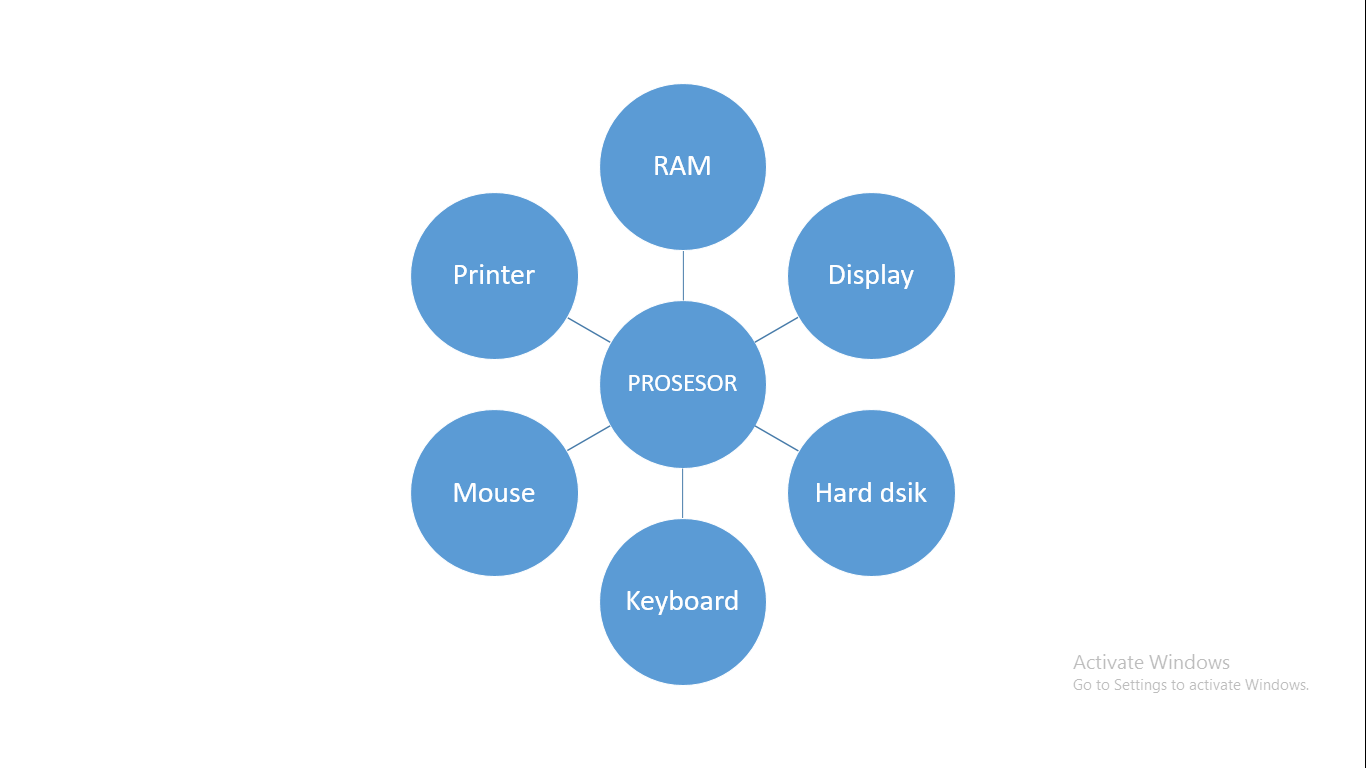
\includegraphics[width=1\textwidth]{figures/komputermodern}}
		\caption{Merupakan struktur dari sebuah mesin Komputer/Hardware untuk menggunakan Komputer.}
		\label{komputermodern}
	\end{figure}
	
	\subsection{Sejarah}
Arsitektur komputer terdokumentasi pertama ada dalam korespondensi antara Charles Babbage dan Ada Lovelace, yang menggambarkan mesin analitis. Saat membangun komputer Z1 pada tahun 1936, Konrad Zuse menjelaskan dalam dua aplikasi paten untuk proyek masa depannya bahwa instruksi mesin dapat disimpan dalam penyimpanan yang sama yang digunakan untuk data, yaitu konsep program tersimpan. \cite{faberkonrad} Dua contoh awal dan penting lainnya adalah:
\begin{itemize}
\item Makalah karya John von Neumann tahun 1945, Draft Pertama Laporan tentang EDVAC, yang menggambarkan sebuah organisasi elemen logis; \cite{von1945first}
\item Kalkulator Elektronik Kalkulator Alan Turing yang lebih rinci untuk Mesin Komputasi Otomatis, juga 1945 dan yang mengutip makalah John von Neumann. \cite{copeland2005alan}
\end{itemize}

Istilah \"arsitektur\" dalam literatur komputer dapat dilacak pada karya Lyle R. Johnson, Frederick P. Brooks, Jr., dan Mohammad Usman Khan, semua anggota departemen Organisasi Mesin di pusat penelitian utama IBM pada tahun 1959. Johnson telah kesempatan untuk menulis sebuah komunikasi riset eksklusif tentang Stretch, sebuah superkomputer yang dikembangkan IBM untuk Laboratorium Nasional Los Alamos (yang saat ini dikenal sebagai Laboratorium Ilmiah Los Alamos). Untuk menggambarkan tingkat detail untuk membahas komputer mewah, dia mencatat bahwa deskripsi format, jenis instruksi, parameter perangkat keras, dan perangkat tambahan kecepatannya berada pada tingkat \"arsitektur sistem\" - istilah yang nampaknya lebih berguna daripada \"organisasi mesin.\"
Arsitektur komputer, seperti arsitektur lainnya, adalah seni untuk menentukan kebutuhan pengguna suatu struktur dan kemudian merancang untuk memenuhi kebutuhan tersebut seefektif mungkin dalam batasan ekonomi dan teknologi.
Brooks melanjutkan untuk membantu mengembangkan IBM System / 360 (sekarang disebut IBM zSeries) baris komputer, di mana \"arsitektur\" menjadi kata benda yang mendefinisikan \"apa yang pengguna perlu ketahui\". Kemudian, pengguna komputer menggunakan istilah ini dengan banyak cara yang kurang eksplisit. \cite{hellige2004genese}
Arsitektur komputer paling awal dirancang di atas kertas dan kemudian langsung dibangun ke dalam bentuk perangkat keras terakhir. \cite{copeland2005alan} Kemudian, prototip arsitektur komputer secara fisik dibangun dalam bentuk komputer logika transistor-transistor (TTL) - seperti prototip dari 6800 dan PA-RISC yang diuji, dan di-tweak, sebelum melakukan sampai pada bentuk perangkat keras terakhir. Pada tahun 1990an, arsitektur komputer baru biasanya \"dibangun\", diuji, dan di-tweak-di dalam beberapa arsitektur komputer lainnya di simulator arsitektur komputer; atau di dalam FPGA sebagai mikroprosesor yang lembut; atau keduanya-sebelum melakukan ke bentuk perangkat keras terakhir. \cite{hellige2004genese}
	\subsection{Pembahasan Arkom}
	\subsection{Survey dari Pararel Arsitektur Komputer}
	Sebuah usaha dibuat untuk mengganti inovasi arsitektur terbaru,dengan konteks pengembangan arsitektur parael yang lebih luas dengan menyurvei fundamental arsitektur komputer dari yang lebih baru dan lebih mapan dan dengan menempatkan alternatif arsitektur ini dengan kerangka kerja yang koheren.
	Penekanan utama adalah pada konstruksi arsitektural daripada mesin paralel yang spesifik.
	Tiga kategori arsitektur yang didefinisikan dan didiskusikan: arsitektur sinkron, terdiri dari vektor, SIMD (single-instruction-stream, multiple-data-stream) dan mesin sistolik; MIMD (multiple-instruction-stream, multiple-data-stream) dengan memori terdistribusi atau shared; dan paradigma berbasis MIMD, terdiri dari tipe hibrida MIMD / SIMD, dataflow, reduction, dan wavei.\cite{duncan1990survey}

	\subsection{Pengurangan Instruksi Instruksi Komputer untuk VLSI}

	Sirkuit terintregasi menawarkan implementasi sistem digital yang kompak dan murah dan menyediakan perfoma melalui keuntungan. 
	Komunikasi on-chip bandwidth tinggi terhadap mereka.saat ini teknologi sedang di gunakan membuat tujuan umum von Neumann processor. 
	Sebaiknya integrasikan sebanyak mungkin mengunakan fungsi pada satu chip, sehingga meminimalkan komunikasi off-chip.
	Bahkan dalam sirkuit Large Scale Integrated (VLSI), transistor yang tersedia di area chip terbatas merupakan sumber daya langka saat digunakan untuk implementasi prosesor atau bahkan komputer yang lengkap, dan karenanya, penggunaannya harus efektif.
	Disertasi ini menunjukkan bahwa tren baru dalam arsitektur komputer terhadap rangkaian instruksi peningkatan kompleksitas menyebabkan penggunaan sumber daya langka yang tidak efisien.
	Kami menyelidiki alternatif arsitektur Computer Instruction Instruction Set (RISC) yang memungkinkan penggunaan transistor on-chip secara efektif dalam unit fungsional yang menyediakan akses cepat ke operan dan instruksi yang sering digunakan.
	Dalam disertasi ini, sifat perhitungan tujuan umum dipelajari, menunjukkan kesederhanaan operasi yang biasanya dilakukan dan frekuensi akses operan yang tinggi, banyak di antaranya dibuat pada beberapa variabel prosedur skalar lokal. 
	Arsitektur prosesor RISC I dan II dipresentasikan. Mereka menampilkan instruksi sederhana dan file register multi-jendela besar, yang jendela tumpang tindihnya digunakan untuk menyimpan argumen dan variabel skalar lokal dari prosedur yang paling baru diaktifkan. 
	Dalam kerangka proyek RISC, yang telah menjadi upaya tim besar di UC Berkeley selama lebih dari tiga tahun, sebuah prosesor single-chip RISC II nMOS dilaksanakan, bekerja sama dengan R. Sherburne. 
	Ersitekturrsitektur mikro-nya dijelaskan dan dievaluasi, diikuti dengan diskusi tentang metode debugging dan pengujian yang digunakan. Teknologi VLSI masa depan akan memungkinkan integrasi sistem yang lebih besar pada satu chip tunggal.
	Pemanfaatan yang efektif dari transistor tambahan dipertimbangkan, dan diusulkan agar digunakan dalam mengimplementasikan unit pengambilan dan urutan instruksi khusus yang terorganisir dan.
	Studi dan evaluasi arsitektur RISC II, serta disain, tata letak, dan pengujian setelah fabrikasi, telah menunjukkan kelayakan dan keuntungan dari pendekatan RISC. Prosesor single-chip RISC II terlihat berbeda dari prosesor komersil populer lainnya.
	transistor ini kurang total, hanya menghabiskan 10\% area chip untuk kontrol daripada satu setengah sampai dua pertiga, dan dibutuhkan desain kurang lebih lima kali lipat dan lay-out usaha untuk mendapatkan hasil yang hampir sempurna.\cite{katevenis1983reduced}

	\subsection{Pemodelan Kinerja Jaringan Komunikasi dan Arsitektur Komputer (Komputer Internasional)}

	Dalam kemajuan teknologi, kemampuan dalam berkomunikasi menjadi lebih rumit dengan kecepatan dan kapasitas yang semakin besar. 
	dengan semakin berkembangnya ilmu komunikasi, ini dapat membuat perkembangan kinerja arsitektur komputer semakin rumit karena harus dibandingkan 
	dengan kecepatan transfer.\cite{harrison1992performance}

	\subsection{MinneSPEC: Sebuah Benchmark SPEC SPEC untuk Proyek Simulasi Berbasis Arsitektur Komputer}

	Arsitektur komputer harus menetukan secara dengan benar mengunakan sumber komputasi yaitu algoritma yang di gunakan untuk menemukan suatu cara dalam memacahkan masalah dari sebuah data input
	Untuk menfasilitasi sebagai benchmarkprogram yang telah di kembangkan inputset MinneSPEC untuk rangkainya adalah benchmark SPEC CPU 2000 untuk beban kerjanya  memungkinkan arsitektur komputer mendapat hasil simulasi dengan waktu yang tepat.
	Ini ada tolak ukurnya  yang valid untuk penelitian berbasis simulasi. 
	Dalam proses pengembangan datasheet, MinneSPEC telah mengukur perhitungan,bentuk pola eksekusi tingkat fungsinya, dengan campuran instruksi,dan perilaku memori dibandingkan dengan program SPEC saat dijalankan dengan masukan referensi.\cite{kleinosowski2002minnespec}

	\subsection{Kebutuhan memori untuk arsitektur komputer yang seimbang}

	Salahlah satu dari akibatnya arsitektur komputer yang seimbang  adalah untuk menyeimbangkan linear rangkaian pe linear untuk melalukakn perhitungan matriks dan matriks trigulzisasi ukuran masing-masing memori lokal PE harus tumbuh secara linier.
	Jadi, semakin besar arraynya, semakin besar setiap memori lokal PE.\cite{kung1986memory}

	\subsection{Arsitektur komputer paralel untuk pemrosesan gambar}

	masalah pengolahan data melibatkan susunan data struktur cukup besar dan kebutuhan pengitungan sangat cepat skema pemrosesan pararel  kusus telah berevolusi selama 20 tahun 
	Sistem paralel yang telah dikembangkan untuk pengolahan citra digariskan dan fitur arsitektur.
	Sebagian besar arsitektur khusus dapat diklasifikasikan secara longgar seperti struktur SIMD atau pipa meskipun beberapa struktur MIMD telah dirancang untuk menganalisis citra tingkat yang  tinggi
	Dalam beberapa tahun terakhir beberapa skema multiple SIMD (MSIMD) telah diusulkan sebagai arsitektur yang sesuai untuk pemrosesan gambar.
	Pengembangan sistem MSIMD yang efektif dibahas dan model komputasi SIMD / MIMD.\cite{reeves1984parallel}

	\subsection{Blok berorientasi pengolahan operasi database relasional di arsitektur komputer modern}

	Sistem basis data tidak  akan sesuai untuk memanfaatkan arsitektur prosesor superscalar  yang modern Secara khusus, jam per instruksi (CPI) untuk query database yang agak sederhana cukup buruk dibandingkan dengan kernel ilmiah atau benchmark SPEC.
	Kurangnya kinerja sistem database disebabkan oleh rendahnya utilisasi cache dan unit fungsi prosesor serta hukuman percabangan yang lebih tinggi
	teknik pemrosesan yang berorientasi blok untuk evaluasi ekspresi agregasi dan operasi pemilahan sebagai fitur dalam sistem.\cite{padmanabhan2001block}

	\subsection{Arsitektur komputer RISC dikonfigurasi untuk meniru set instruksi komputer target}

	komputer arsitektur risc dikonfigurasi untuk meniru set intruksi komputer target untuk menjalankan perangkat lunak yang di tulis untuk komputer target, misalnya intel 80x86, motorola 680x0 atau mips R3000. 
	aparatus terintegrasi dengan komputer risc inti untuk membentuk komputer yang mengeksekusi intruksi risc yang di perluas.
	intruksi risc yang di perluas berisi bidang data yang menunjuk register tidak langsung yang mengarah ke register emulasi paling tidak sama dengan yang ada di komputer target. 
	namun, bidang dalam intruksi risc yang diperluas membatasi lebar yang ditiru dan dibutuhkan oleh intruksi yang ditiru tertentu.
	selain itu, intruksi risc yang diperluas berisi bidang yang menunjuk mode emulasi untuk kde kondisi dan memilih logika agar sesuai dengan kode kondisi komputer target. 
	intruksi target diurai dan dikirim ke urutan satu atau lebih intruksi risc yang diperluas untuk meniru setiap intruksi target.\cite{scantlin1996risc}

	\subsection{Database Arsitektur Komputer untuk Memanage sebuah program penghargaan dan mendapatkan pembayaran}

	Sistem distribusi informasi yang canggaih termasuk ke dalam jalur komunikasi yang mempunyai beberapa switching komunikasi selektif. 
	Hal itu menentukan apakah transaksi elektronik tersebut layak diterima atau tidak.
	Sistem komputer,yang intensif dapat mencakup titik sistem pengolahan yang menghasilkan laporan yang baik sesuai dengan kriteria yang di setujui.\cite{robinson1998database}

	\subsection{Arsitektur komputer berkinerja tinggi}

	Sebagian besar aktivitas perancangan komputer telah beralih ke komputer desain berkinerja tinggi,karena komputer desktop single-user mencapai titik pengiriman daya komputer lebih banyak dari pada mainframe yang lama.
	Karena akan lebih mudah untuk Topik yang dibahas meliputi: Pendekatan arsitektur umum seperti desain memori, teknik pipa, dan struktur paralel. 
	kemacetan mendasar seperti bandwidth memori, bandwidth proses, komunikasi, dan sinkronisasi, teknik evaluasi, contoh aplikasi nyata dan persyaratan arsitekturalnya.\cite{stone1987high}

	\subsection{Ifrastruktur untuk pemodelan sistem komputer}

	Perangcang dapat menjalankan program pemodelan perangkat, model perangkat lunak untuk memvalidasi kinerja dan ketepatan desain perangkat keras.
	pemrogram dapat menggunakan model  untuk mengembangkan dan menguji perangkat lunak sebelum perangkat keras sebenarnya tersedia.
	Tiga persyaratan penting mendorong penerapan model perangkat lunak: kinerja, fleksibilitas, dan detail. 
	Kinerja menentukan jumlah beban kerja yang dapat dilakukan model mengingat sumber daya mesin tersedia untuk simulasi.
	perangkat simplecar memiliki sebuah infrastruktur simulasi dan pemodelan arsitektural.
	Simulator SimpleScalar mereproduksi operasi sebuah  perangkat komputer dengan menjalankan instruksi program menggunakan penerjemah.
	instruktur instruksi telah mendukung :instruksi populer,termasuk alpha,PPC, x86, dan ARM.\cite{austin2002simplescalar}
	Bagian bagian arsitektur komputer
	Ini merupakan bagian-bagian arsitektur komputer\ref{sasasa}
		1 Software - perangkat lunak yang menjalankan hardware
		2 kernell - jembatan antara software dengan hardware
		3 Hardware - perangkat keras untuk menjalankan operasi komputer
    \begin{figure}[ht]
		\centerline{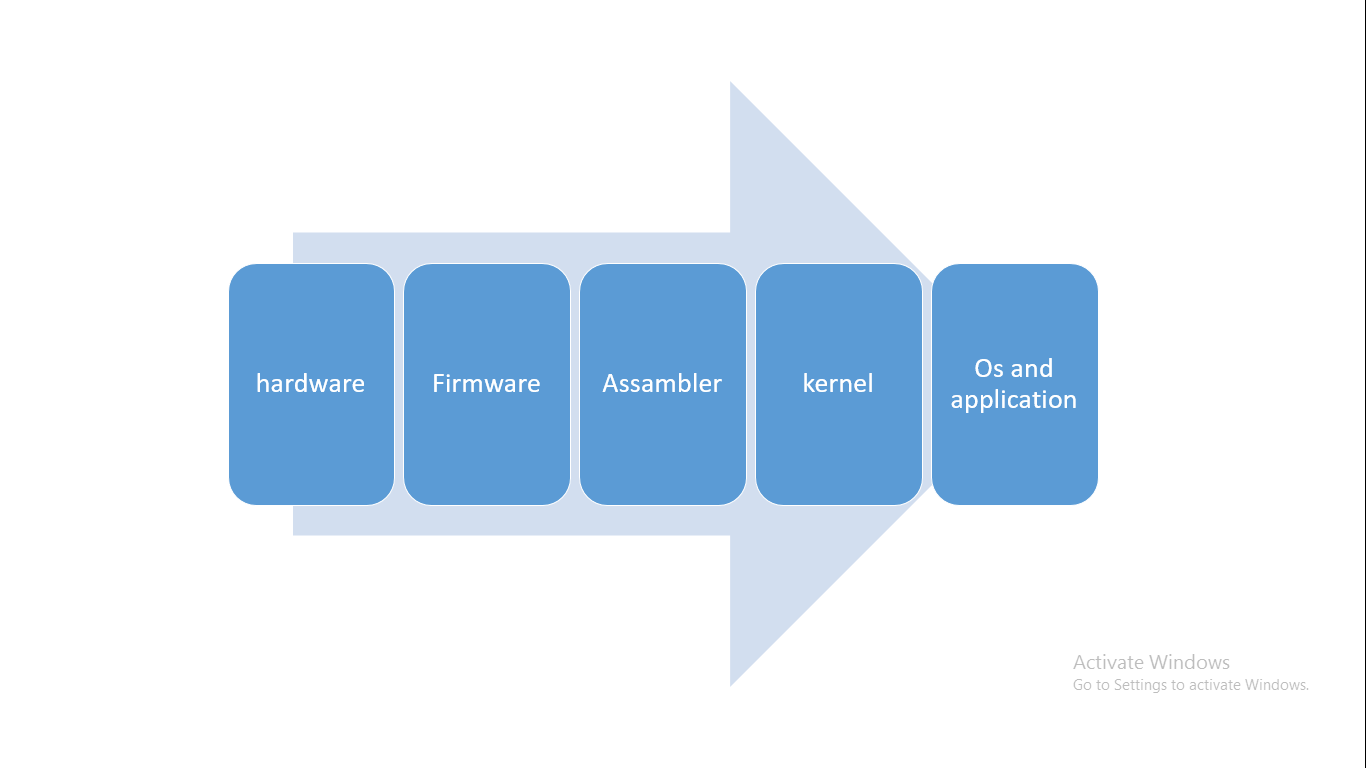
\includegraphics[width=1\textwidth]{figures/sasasa.PNG}}
		\caption{Bagian dari Arsitektur Komputer}
		\label{sasasa}
	\end{figure}
	
	\subsubsection{PENUTUP}
	\subsubsection{Fungsi dari Arsitektur Komputer}
	Sebuah tolak ukur untuk mengevaluasi Arsitektur Komputer berkinerja tinggi pada aplikasi Bioinformatika.
	Pertumbuhan eksponensia telah mendorong minat yang meningkat dalam informasi genetika berskala besar. 
	aplikasi bioinformatika, adalah aplikasi untuk memudahkan peneliti menyaring data data biologis secara besar besaran dan untuk mengekstrak informasi yang berguna, menjadi beban komputer yang semakin penting.
	Aplikasi tersebut sebagai perwakilan untuk perancangan dan evaluasi arsitektur komputer berkinerja tinggi untuk beban kerja yang muncul pada saat ini.
	saat ini, suite BioPerf berisi kode dari 10 paket bioinformatika yang sudah sangat populer yang mencakup bidang studi utama biologi komputer yaitu perbandingan urutan, rekonstruksi filogenetik,prediksi struktur protein, dan homologi urutan dan penemuan gen.\cite{bader2005bioperf}
	\subsubsection{Arsitektur Komputer untuk pemrosesan kecerdasan buatan}
	Artikel ini menilai pendekatan arsitektural yang berbeda terhadap disain komputer untuk aplikasi kecerdasan buatan (artificial intelligence / AI).
	perbandingan mesin ai dengan komputer numrik Penekanannya adalah pada tiga kelas arsitektural: multiprocessors yang mendukung operasi MIMD (multiple-instruction stream dan multiple-stream data) interaktif melalui ruang memori bersama.
	multicomputers yang mendukung operasi SISD (single-instruction stream dan single-data stream) melalui pesan yang lewat di antara prosesor terdistribusi dengan kenangan lokal; dan komputer serbaguna yang terdiri dari sejumlah besar node memori prosesor butiran halus yang beroperasi di SIMD (aliran instruksi tunggal dan aliran data ganda), SIMD multipel, atau mode MIMD.\cite{hwang1987computer}
	
	\subsubsection{KESIMPULAN}
	\subsubsection{Kesimpulan}
	Jadi, arsitektur komputer adalah sebuah awal dari terbentuknya software dan hardware dari komputer yang dapat dirubah atau dirancang untuk mengubah logika manusia ke dalam logika atau bahasa komputer.
	jika kita tidak memahami arsitektur komputer maka komputer tidak akan terbentuk secara sempurna dan arsitektur komputer merupakan awal dari lahirnya mesin komputer untuk membantu pekerjaan manusia.
	



\chapter[Software]
{Software\\ software}
%Software (Arsitektur Komputer)
%Kelas : D4 TI 1B
%Khadijah Hasanah Putri Harahap 1174022
%Liyana Majdah Rahma 1174039
%Luthfi Muhammad Nabil 1174035
%Nisrina Aulia Firdaus 1174098
%Salwaa Tania 1174047
%Septia Rahayu 1174044
%Diana Satima Gistivani 1154018




\section{Definisi Software}
Software secara singkat ialah sebuah aplikasi yang terdapat pada computer maupun perangkat lunak berbasis elektronik lainnya. Fungsi dari Software sendiri cukup beragam dan mampu diterima oleh masyarakat pada umumnya. Dan berikut adalah Definisi, fungsi, bahkan Sejarah dari perkembangan Software itu sendiri.

\begin{figure}[ht]
\centerline{
\includegraphics[width=0.5\textwidth]{figures/Abstraksi.jpg}}
\caption{Sistem Operasi}
\label{Abstraksi}
\end{figure}
\begin{flushleft}
Software adalah instruksi langsung untuk computer ataupun perangkat elektronik lain yang dapat ditemukan di berbagai tempat dan pemakaian yang beragam seperti Software sebagai pendeteksi detak jantung di rumah sakit ataupun Software hiburan seperti video games. Pada gambar \ref{Abstraksi} terlihat sebuah tampilan software Sistem Operasi. Produk Software sendiri memiliki berbagai macam jumlah kode baik dari yang hanya ratusan kode maupun jutaan kode yang diharapkan dapat melakukan pekerjaan secara efisien untuk para pengguna dari aplikasi tersebut. Software sendiri merupakan inti dari computer karena untuk mengoperasikan sebuah Komputer haruslah dalam computer tersebut memiliki perangkat keras. Software sendiri bersifat bisa terbaca namun tidak berwujud umumnya perangkat keras yang memang pada dasarnya bisa disentuh. 
\end{flushleft}
\begin{flushleft}
Software dibuat oleh seorang Perekayasa Perangkat Lunak  atau yang sering disebut sebagai Programmer. Programmer sendiri bertugas membuat sebuah Software sesuai dengan kebutuhan dari seorang klien maupun Programmer itu sendiri dan menerapkan beberapa Teknologi yang ada untuk dipakai oleh Programmer itu sendiri dan juga melakukan pemeliharaan Software yang telah dibuatnya jika Programmer tersebut diposisikan sebagai Pengembang Software. Teknik Rekayasa Software sendiri dapat meningkatkan efisiensi dan memberikan kemudahan bagi Pengembang Software dalam mengembangkan sebuah Software yang telah dibuat. 
\end{flushleft}
\begin{flushleft}
Pembuatan Software sendiri dibuat menggunakan bahasa pemrograman yang dibuat oleh programmer yang kemudian disusun (compile) sehingga membentuk kode-kode yang bisa dibaca oleh perangkat keras. Software dibuat untuk memenuhi kebutuhan – kebutuhan tertentu sesuai dengan perkembangan zaman. Software berfungsi untuk memproses data, Instruksi atau perintah yang nantinya menghasilkan sebuah hasil (Output) sesuai kebutuhan. Selain itu Software juga berfungsi sebagai penghubung antara pengguna dengan perangkat keras.
\end{flushleft}

\section{Sejarah Perkembangan Software}
\begin{flushleft}
Software telah berkembang melalui empat era yang terjadi sejak tahun 1950 sampai sekarang. Setiap era memiliki karakteristik khusus dan setiap tahunnya Software mengalami peningkatan, baik dari kompleksitas, ukuran, teknologi, dan efisiensinya dalam melakukan pekerjaan. 
\end{flushleft}
\begin{flushleft}
Krisis Software pernah terjadi pada tahun 1960 karena praktik Rekayasa Software masih kurang dapat diterima. Tahap awal Software sendiri memunculkan banyak minat pada computer, walaupun banyak kode yang ditulis, tetapi tidak ada standar yang ditetapkan. Lalu pada awal tahun 1970-an, banyak program computer mulai mengalami kegagalan dan banyak orang kehilangan kepercayaan pada sebuah Software sehingga krisis Software diumumkan. Alasan yang mengarah pada krisis adalah sebagai berikut :
\begin{itemize}
	\item Perkembangan perangkat keras yang lebih cepat
	\item Kemampuan untuk membangun yang dituntut untuk memenuhi kebutuhan secara cepat
	\item Meningkatnya ketergantungan pada Software
	\item Desain yang kurang dan minimnya teknologi maupun Sumber Daya Manusia
\end{itemize}
\end{flushleft}
\begin{flushleft}
Walaupun krisis Software teridentifikasi pada awal-awal tahun, tetapi pada tahun-tahun sebelumnya sudah pernah terjadi kegagalan Software di seluruh dunia. Software pada dasarnya di anggap gagal jika proyek pembuatan tersebut dihentikan karena faktor kekurangan biaya atau melewati jadwal yang telah ditentukan atau jika proyek melebihi 50 persen dari perencanaan. Beberapa contoh kegagalan Software mencakup kegagalan system control lalu lintas, kegagalan Software medis, kegagalan Software telekomunikasi, dan sebagainya. Alasan utama kegagalan yang lainnya adalah dikarenakan pengadopsian Praktik Rekayasa Software yang buruk. Beberapa praktik Software yang buruk meliputi : 
\begin{itemize}
	\item Tidak adanya histori pengukuran Software
	\item Penolakan dari keakuratan perkiraan daya
	\item Gagalnya penggunaan alat untuk perencanaan dan memperkirakan secara otomatis
	\item Praktik yang berlebihan
	\item Jadwal yang tidak logis
	\item Kegagalan menggunakan desain review dan inspeksi kode
\end{itemize}
\end{flushleft}
\begin{flushleft}
Untuk menghindari kegagalan dan meningkatkan kepercayaan dari masyarakat, dibutuhkan pemahaman yang baik dari proses tersebut, penyusunan jadwal yang ditargetkan untuk pembuatan sebuah Software yang terbaik dan mengukur biaya yang sebanding maupun kualitas yang dibutuhkan. Suatu proses Software merupakan serangkaian kegiatan, metode, dan praktik – praktik yang melibatkan transformasi yang dilakukan orang untuk mengembangkan dan memelihara sebuah Software. 
\end{flushleft}
\begin{flushleft}
Saat ini kebanyakan masalah terjadi dikarenakan adanya proses Software yang kacau dan terkadang keberhasilan Software tergantung pada usaha perorangan. Oleh karena itu, dibutuhkan pengalihan focus dari sebuah produk kepada proses karena terfokus kedalam produk cenderung mengabaikan masalah skalabilitas dan hanya akan melakukan perbaikan pada system yang ada. Selain itu, alasan tersebut bisa berkaitan dengan prinsip – prinsip Rekayasa Software apabila kebutuhan teridentifikasi dengan benar. Apabila identifikasinya benar, maka akan memudahkan dalam mengidentifikasi teknik atau praktik terbaik yang dapat diterapkan kepada Software karena satu proses bisa saja cocok untuk satu organisasi dan bisa tidak cocok untuk sebagian lainnya. Perkembangan dari sebuah Software berproses melalui beberapa era, diantaranya :
\begin{enumerate}
	\item Era Pioner/Pemula (Tahun 1950-1960) \\	
Dalam era ini, bentuk dari Software masih berbentuk sambungan kabel ke bagian – bagian pada computer. Pengaksesan computer sendiri masih dilakukan dengan <i>punched card</i>, yaitu kartu yang dilubangi. Penggunaan computer pada saat itu masih dilakukan secara kontak langsung. Software pada era ini masih menyatu dengan perangkat kerasnya dan hanya menghasilkan sebuah hasil berupa cetakan. Pengaplikasian pada masa ini pun masih terbilang hanya untuk keperluan yang tidak begitu banyak dikarenakan teknologi yang masih terbilang sangat kuno, seperti untuk membuat alat perhitungan matematika yang digunakan oleh ilmuwan untuk menyelesaikan operasi matematika secara cepat. 
	\item Era Stabil (Tahun 1960-1970) \\
Dalam era ini, pengguna computer sudah sangat meningkat, tidak hanya oleh kalangan peneliti tetapi juga oleh kalangan industri. Perusahaan Software pun mulai bermunculan dan sebuah Software dapat menjalankan beberapa ini. Di era ini, Software mulai bisa dibilang terpisah dari perangkat kerasnya dan bisa dikenal sebagai sebuah produk. Kode perintah Software yang dijalankan oleh computer pun tidak lagi satu-satu, tetapi sudah menampilkan banyak proses yang dilakukan secara serempak. Sebuah Software juga bisa digunakan oleh banyak pengguna secara cepat. Pada era ini juga basis data yang berfungsi menyimpan sebuah data mulai diperkenalkan.
	\item Era Mikro (Tahun 1970-1980) \\
Pada era ini, Software mulai berkembang sebagai perangkat yang dapat memenuhi kebutuhan perseorangan. Software juga dapat dibedakan menjadi Software system yang bertugas menangani sisi internal seperti Sistem Operasi dan Software aplikasi yang dapat digunakan langsung oleh penggunanya untuk keperluan tertentu. 
	\item Era Modern (Tahun 1980-Sekarang) \\
Pada era yang kita alami sekarang, Software sudah dapat dijangkau di berbagai perangkat elektronik, bahkan sebuah computer genggam atau telepon genggam terdapat sebuah aplikasi yang dapat disambungkan atau disinkronkan dengan computer. Bahkan telepon, TV, mesin cuci, dan Oven sekalipun terdapat Software yang berfungsi untuk mengatur operasi dari perangkat keras. Bahkan semua peralatan tersebut bisa dipantau dan diatur hanya menggunakan sebuah telepon genggam. Pembuatan Software bukan lagi pekerjaan yang hanya dilakukan oleh segelintir orang, tetapi telah menjadi pekerjaan banyak orang dengan teknik yang dibilang cukup memadai. Teknologi yang berkembang juga membantu orang awam untuk mempelajari bagaimana cara untuk membuat Software sendiri. Software sendiri sekarang memiliki fitur suara dan tampilan gambar.
\end{enumerate}
\end{flushleft}
\section{Dampak dari munculnya Software}
\begin{flushleft}
Software pada masa dulu dan sekarang sudah sangat mempengaruhi masyarakat dan budaya yang selalu dilakukan dalam berinteraksi ataupun melakukan sebuah pekerjaan. Seiring teknologi mulai berkembang, dampak dari munculnya Software mulai sangat drastis dibandingkan dengan tidak adanya Software. Faktor dari Software yang mempengaruhi masyarakat salah satunya yaitu : 
\begin{enumerate}
	\item Faktor Ekonomi\\
	Software pada masa emasnya memimpin produktivitas dan total nilai produksi barang. Seperti di Amerika Serikat, Software memimpin sekitar ¼ dari semua peningkatan total nilai produksi barang pada tahun 1990-an (atau sekitar 90 Miliar Dollar per tahun) dan 15 persen dari semua pertumbuhan produktivitas pada akhir tahun 1990-an (atau sekitar 33  Miliar Dollar/tahun).
	\item Faktor Sosial\\
Munculnya Software mulai mengubah budaya masyarakat yang sebagian besar mulai menggunakan computer. Dengan adanya E-mail, World Wide Web, dan pesan singkat memungkinkan orang untuk berinteraksi dengan cepat dari semua tempat terjauh sekalipun dan mengurangi biaya dari sebuah pesan singkat. 
Kesuksesan dari Software juga telah diterapkan yang mencakup Linux, Space Shuttle Software, dan Automatic Teller Machine (ATM)	
\end{enumerate}
\end{flushleft}
\section{Jenis - Jenis Software}
\begin{flushleft}
Software adalah sebuah program computer yang berfungsi sebagai penghubung antara pengguna dan perangkat keras. Software juga dapat disebut sebagai penerjemah instruksi yang dijalankan pengguna computer untuk dikirim ke perangkat keras. Software dibagi menjadi tiga bagian, yaitu program Aplikasi, Sistem Operasi, dan Bahasa Pemrograman. 
\end{flushleft}
\subsection{Software Antivirus}
\begin{flushleft}
Software ini berfungsi untuk mendeteksi dan menghapus virus computer system computer. Software ini juga dapat menentukan apakah sebuah system computer telah terinfeksi atau terdapat adanya sebuah virus atau tidak. Antivirus biasanya melakukan pemindaian secara otomatis pada system computer ke semua berkas yang bisa diakses. Pergerakan mencurigakan dari sebuah aplikasi juga dapat terdeteksi oleh Antivirus dan bisa dicurigai oleh Antivirus sebagai sebuah program yang mencurigakan. Antivirus adalah Software yang termasuk kedalam bagian dari program aplikasi.
\end{flushleft}
\subsection{Software Bisnis}
\begin{flushleft}
Software ini berfungsi sebagai program untuk melakukan sebuah pekerjaan kantoran seperti menyiapkan presentasi, membuat sebuah dokumen statistika, dan sebagainya. Aplikasi ini sangat sering digunakan oleh pekerja kantoran bahkan sampai akademisi atau pelajar masa kini. Contoh dari aplikasi yang sering digunakan adalah Microsoft Office dan Open Office.
\end{flushleft}
\subsection{Software Desain Grafis}
\begin{flushleft}
Desain Grafis juga dipermudah dengan adanya Software khusus untuk Desain Grafis di computer. Seperti Aplikasi Adobe Photoshop yang mampu mengubah gambar yang ada menjadi sesuatu sesuai keinginan sang editor. Bahkan Foto yang telah di scan dapat di edit memakai Aplikasi ini dan dapat dicetak setelahnya atau dijadikan simpanan di computer. 
\end{flushleft}
\subsection{Software Grafis 3D}
\begin{flushleft}
Dengan adanya Software ini, sebuah gambar 3 Dimensi dapat dibuat bahkan dapat digerakkan seperti film anak – anak yang menggunakan karakter 3 Dimensi atau Pembuatan kerangka bangunan 3 Dimensi. Aplikasi yang sering dipakai saat ini adalah AutoCAD atau 3DS Max yang dikembangkan oleh Autodesk. AutoCAD banyak digunakan oleh Insinyur Sipil, Pengembang lahan, Desainer, Animator, dan lain – lain. 
\end{flushleft}
\subsection{Software Grafis}
\begin{flushleft}
Seperti halnya dengan Software Desain Grafis hanya saja Software Grafis dipakai untuk membuat sebuah grafis visual seperti diagram aliran (flowchart), brainstorm, dan Skema Jaringan. Contoh dari aplikasi Software Grafis seperti Microsoft Visio yang dibuat oleh Visio Corporation yang diakuisisi oleh Microsoft. Sebagian besar yang memakai aplikasi ini adalah seorang perancang sebuah proyek. 
\end{flushleft}
\subsection{Software Jaringan}
\begin{flushleft}
Dengan ketersediaan sebuah Jaringan membuat informasi yang ada di sebuah Website atau sebuah komunikasi melalui pesan singkat atau surat elektronik (E-Mail) mulai bermunculuan. Bahkan aplikasi Chatting seperti Yahoo! Messengger dan AOL mulai meledak penggunaannya karena dapat melakukan Chatting secara langsung (Realtime). Pemakai dari aplikasi ini sangat banyak digunakan oleh kalangan masyarakat.
\end{flushleft}
\subsection{Software Kompresi Data}
\begin{flushleft}
Software ini berfungsi sebagai pengompres sebuah file/data yang besar maupun mengelompokkan file – file kecil menjadi satu Archive yang berukuran lebih kecil dari total semua file kecil. Aplikasi ini banyak digunakan karena mampu membuat atau mengorganisir file – file biasa menjadi satu file berformat Archive. Contoh aplikasinya seperti WinZip, WinRAR.
\end{flushleft}
\subsection{Software Musik}
\begin{flushleft}
Untuk musik pun ada Software yang khusus untuk Memutar bahkan mengubah Musik. Tidak hanya pada computer, bahkan telepon genggam pun terdapat aplikasi Pemutar Musik. Dengan adanya aplikasi ini kita tidak perlu memutar sebuah Tape atau Cakram untuk mendengarkan atau menyimpan musik melainkan cukup menyimpan atau mendownload musik dari Jaringan Internet dan memutarnya menggunakan aplikasi musik. Pengguna aplikasi ini banyak di kalangan masyarakat pengguna computer manapun.
\end{flushleft}
\subsection{Software Pembaca Gambar}
\begin{flushleft}
Di setiap Sistem Operasi saat ini sudah banyak memiliki sebuah Software Pembaca Gambar. Gambar sendiri bisa berupa Foto atau Gambar Digital. Dengan aplikasi ini kita dapat melihat gambar di dalam computer. Aplikasi yang sering dipakai untuk melihat gambar seperti Windows Photo Viewer.
\end{flushleft}
\subsection{Software Sistem Operasi}
\begin{flushleft}
Pada era sekarang sebuah Software mulai sangat tidak berwujud atau bisa tersentuh melainkan telah diaplikasikan ke dalam computer. Sistem Operasi sendiri adalah penghubung antara sebuah Software program aplikasi dengan Perangkat Keras pada computer. Dengan adanya Sistem Operasi cukup memudahkan seorang pengembang Software untuk mengembangkan aplikasi yang telah dibuat dan mempermudah masyarakat untuk menjalankan banyak Software secara serentak sesuai dengan kemampuan sebuah computer. Sistem Operasi yang sangat dipakai sekarang adalah Sistem Operasi Windows.
\end{flushleft}
\section{Rangkuman}
\begin{flushleft}
Software telah berkembang dimulai pada tahun 1950 sampai saat ini yang pernah melalui empat  era. Setiap era memiliki peningkatan dan krisis baik dalam ukuran, kompleksitas, maupun kepercayaan masyarakat terhadap Software. Saat ini kebanyakan masalah terjadi dikarenakan proses Software yang kacau bahkan lewatnya jadwal pembuatan membuat sebuah aplikasi dianggap gagal oleh masyarakat. Oleh karena itu, suatu focus pada proses sangat dibutuhkan karena focus pada produk cenderung hanya memperbaiki system yang ada dan mengabaikan masalah skalabilitas.
\end{flushleft}
\begin{flushleft}
Perkembangan Ilmu Pengetahuan dan Teknologi berperan besar sebagai pengubah teknik pembuatan seorang Perekayasa Perangkat Lunak sampai sekarang. Pada saat ini orang tidak perlu  sangat mempermasalahkan sebuah perangkat keras untuk membuat sebuah Software melainkan hanya memperlukan Ilmu yang cukup untuk dapat menggunakan bahasa pemrograman yang akan dikonversi ke bahasa computer. 
\end{flushleft}
\begin{flushleft}
Dengan adanya Software memudahkan masyarakat dalam melakukan pekerjaan tertentu dan bahkan bisa membersihkan sebuah system computer yang terinfeksi oleh sebuah virus. Fungsi dari Software sendiri sudah dipakai oleh Masyarakat biasa sampai Ilmuwan ataupun seorang Dinas social Masyarakat. Jenis – jenis Software juga sangatlah beragam dimulai dari Software Antivirus sebagai Pelindung Sistem Komputer sampai Software Sistem Operasi sebagai penghubung antara Software dan perangkat keras.
\end{flushleft}
Sumber dari artikel dipetik dari buku \cite{simarmata2010rekayasa}


\chapter[Hardware]
{Software\\ hardware}
%Nama Kelompok: Hardware
%Kelas: D4 1B
%Alit Fajar 1174057
%Berlian 1174034
%Ichsan 1174058
%Kevin 1174059
%Iqbal Hambali 1174060
%Virga 1174065

\section{Definisi}
Perangkat keras komputer adalah komponen fisik atau komponen komputer, seperti monitor, keyboard, penyimpanan data komputer, kartu grafis, kartu suara dan motherboard. Sebaliknya, perangkat lunak adalah instruksi yang bisa disimpan dan dijalankan oleh perangkat keras.
Perangkat keras diarahkan oleh perangkat lunak untuk menjalankan perintah atau instruksi apapun. Kombinasi perangkat keras dan perangkat lunak membentuk sistem komputasi yang dapat digunakan
Hardware atau yang kita kenal sebagai perangkat keras adalah suatu perangkat dalam komputer yang dapat dilihat secara langsung maupun dapat
disentuh, perangkat keras ini dapat mendukung berjalannya suatu komputerisasi. Perankat keras dapat bekerja apabila ada perintah yang
dilakukan kepada perangkat keras ini. Secara fisik, perangkat keras memiliki komponen-komponen yang terdiri dari suatu sistem. Sistem
adalah suatu komponen-komponen yang saling berhubungan dan saling mendukung. Jika salah satu komponen tidak berfungsi, maka proses-
proses dalam komputer tidak berjalan dengan baik.

\subsection{Sejarah Hardware}
Hardware atau dalam bahasa Indonesianya perangkat keras pertama kali dikemukakan oleh seorang ilmuan matematik ternama yang berkewarga
kenegaraan Inggris. Namanya Charles Babbage, beliau menciptakan suatu mesin hitung yang disebut difference engine pada tahun 1822.
Belum puas dengan penemuannya tersebut Charles Babbage memulai pengembangan penemuan sebelumnya yaitu difference engine menjadi
analytical engine yang dapat melaksanakan kalkulasi apa saja. Pada tahun 1833 analytical engine pun berhasil Charles Babbage temukan
dan mesin ini dikenal sebagai mesin General Purpose Digital Computer. Charles Babbage pun dikenal sebagai bapak komputer modern.

Belum selesai dari itu pada tahun 1937 seorang profesor ahli matematika dari universitas terkenal Havard Prof. Howad Aikem merancang
pembuatan sebuah komputer yag mampu melakukan operasi aritmatika dan logika secara otomatis. Setelah itu Prof. Howad Aikem memulai
kerjasamanya dengan perusahan IBM pada tahun 1944 untuk menyelesaikan komputer secara elektronik dan dinaminya \"Havard MARK I\" atau
Automatic Sequence Controlle Calculator (ASCC).

Sejarah perkembangan Hardware dapat dibedakan dalam 2 periode yaitu periode sebelum tahun 1940 dan periode sesudah tahun 1940. 
sebelum tahun 1940 dapat dikatakan sebagai evolusi komputer dengan teknologi mekanik. sejarahnya komputer dimulai ketika lahirnya 
komputer generasi yang pertama dengan nama Electronic Numerical Integrator and Calculator atau yang lebih banyak dikenal orang dengan 
nama computer ENIAC, padahal komputer digital pertama sebenarnya adalah Atanasoff-BErry computer atau disingkat dengan ABC,
pendirinya yaitu bernama Vincent Atanasoff.
 
\subsection{Generasi Pertama Perangkat Keras}
sejarahnya komputer dimulai ketika lahirnya 
komputer generasi yang pertama dengan nama Electronic Numerical Integrator and Calculator atau yang lebih banyak dikenal orang dengan 
nama computer ENIAC, padahal komputer digital pertama sebenarnya adalah Atanasoff-BErry computer atau disingkat dengan ABC,
pendirinya yaitu bernama Vincent Atanasoff. Pada generasi yang pertama Dr. John W Mauchly dan rekannya J. Presper Eckert membuat 
komputer yang disebut ENIAC. Electronic Numerical Integrator and Calculator atau ENIAC dibuat 1942, yang tujuan pembuatannya untuk
membantu Amerika Serikat menghitung target sasaran bom pada perang dunia kedua, Electronic Numerical Integrator and Calculator atau 
ENIAC sebenarnya lebih dikenal dengan sebutan Vacum Tube.

\subsection{Genereasi Kedua Perangkat Keras}
Era Vacum Tube sudah mulai tergantikan oleh generasi kedua ini. Pada tahun 1959 Transistor menggantikan Vacum Tube dalam
menyimpan dan melakukan proses informasi. Dikarenakan Transistor memilik bentuk yang lebih kecil dari Vacum Tube, dan juga lebih tenang
dikarenakan tidak mudah panas, serta tidak begitu banyak energi yang dibutuhkan untuk menjalankannya membuat Transistor berhasil mengambil
alih tugas Vacum Tube.

\subsection{Generasi Ketiga Perangkat Keras}
Pada generasi ketiga ini penggunaan perangkat keras IC atau Itegrated Circuit sudah digunakan pada komputer, era IC atau Itegrated Circuit
dimulai tahun 1964 dengan penyimpanan yang berkapasitas dua megabyte dan menggunakan daya listrik yang lebih hemat membuat Itegrated Circuit
menjadi perangkat keras yang digunakan untuk komputer modern. Pada generasi ini software mulai dikenalkan.

\subsection{Generasi Keempat Perangkat Keras}
Pada tahun 1970, setelah penciptaan Itegrated Circuit tujuan pengembangan komputer semakin jelas yaitu seperti, memperkecil ukuran
sirkuit dan komponen-komponen elektrik lainnya. IBM 370 telah menggunkan LSI yang juga merupakan komputer generasi keempat yang pertama.

\subsection{Salah Satu Contoh}

\subsubsection{Prosesor}
Prosesor adalah bagian penting yang berada dalam komputer yaitu sebagai tenaga kerja di dalam komputer. Prosesor terletak dalam slot
yang terletak dalam perangkat inti atau yang lebih dikenal dengan motherboard. Pengaruh prosesor dalam komputer ini ada sebagai kecepatan
komputer yang tergantung oleh jenis dan kapasitas prosesor tersebut. Kapasitas prosesor pada saat ini mencapai GigaHertz (GHz).
Perhitungan tersebut dalam mengolah data atau mengolah informasi. Prosesor ini memiliki beberapa jenis dimana setiap jenis ini memiliki 
keunggulan dan kekurangannya masing-masing.

Dari tahun ke tahun, prosesor ini sudah mengalami peningkatan dan mengalami banyak perubahan yang berarti. Salah satu perubahan yang 
terjadi adalah pada Prosesor Intel yang kini telah mencapai generasi ke 7. Dan pada Prosesor AMD telah mencapai PHENOM II X6. Tapi
bertolak belakang dari itu semua, untuk memiliki prosesor yang baik dan bagus kita harus mengeluarkan biaya yang melebihi dari biaya
prosesor biasa untuk perawatan dan pengadaan prosesor tersebut.

\subsection{Merk Prosesor yang Beredar Di Pasaran}
\begin{itemize}	
	\item AMD,
	\item Apple,
	\item Cyrix VIA,
	\item IBM,
	\item IDT,
	\item Intel,
\end{itemize}

\subsection{Contoh Gambar}

\ref{ARM}
\begin{figure}[ht]
\centerline{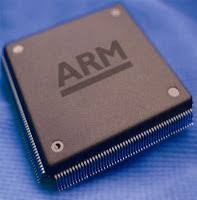
\includegraphics[width=1\textwidth]{figures/ARM.JPG}}
\caption{ARM}
\label{ARM}
\end{figure}

\ref{Cyrix}
\begin{figure}[ht]
\centerline{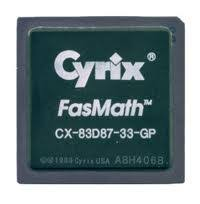
\includegraphics[width=1\textwidth]{figures/Cyrix.JPG}}
\caption{Cyrix}
\label{Cyrix}
\end{figure}

\ref{i5}
\begin{figure}[ht]
\centerline{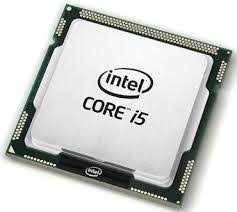
\includegraphics[width=1\textwidth]{figures/i5.JPG}}
\caption{i5}
\label{i5}
\end{figure}

\ref{IntelPentium}
\begin{figure}[ht]
\centerline{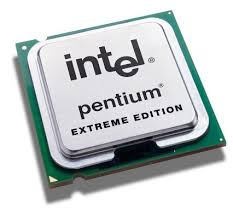
\includegraphics[width=1\textwidth]{figures/IntelPentium.JPG}}
\caption{IntelPentium}
\label{IntelPentium}
\end{figure}

\subsection{Komponen Prosesor}
Prosesor adalah komponen yang terpenting dari sistem komputer, ia juga merupkan pengolah data berdasarkan instruksi yang diberikan kepada
prosesor tersebut,dalam mewujudkan fungsi dan tugasnya prosesor tersusun atas beberapa komponen sebagai anggota dari setuktur CPU, yaitu

\begin{itemize}
	\item Arithmatic dan Logic Unit
	Bertugas untuk membentuk fungsi-fungsi pengolhan data komputer, Arithmatic dan Logic Unit sering disebut sebagai Machine Language
	(mesin bahasa) karena bagian ini mengerjakan instruksi bahasa mesin yang diberikan kepadanya. Arithmatic dan Logic Unit terdiri
	dari dua bagian, yaitu Unit Arithmatika dan Unit Logika Boolean.
	\item Control Unit
	Control Unit bertugas mengontrol operasi CPU dan mengontrol secara keseluruhan komputer, sehingga terjadi sinkronisasi antar komponen
	dalam menjalankan setiap fungsi operasinya.
	\item Register
	Register adalah media penyimpanan internal CPU yang digunakan dalam proses mengolahan data. Memori ini sifatnya sementara biasanya
	digunakan untuk menyimpan data saat dilakukan pengolahan data.
	\item CPU Inter Connections
	Merupakan sistem koneksi dan bus yang menghubungkan komponen internal CPU.
\end{itemize}

\subsection{Perawatan yang Baik Sesuai Prosedur Pabrik}
Hardware atau perangkat keras pada laptop atau komputer merupakan bagian vital yang amat perlu dirawat. 
Seperti halnya prosesor, hard disk, keyboard, layar monitor, baterai, dan sebagainya. 
Semua itu adalah bagian-bagian penting dari komputer yang perlu di perhatikan dan dirawat secara rutin, misalnya
diharapkan agar selalu tidak lupa untuk mengolesi pasta pada bagian atas processor lebih kurang setiap 3 bulan sekali,
casing pc yang memiliki jalur sirkulasi udaranya karena apabila casing tidak memiliki jalur sirkulasi maka komponen yang 
ada didalam pc anda akan lebih cepat panas termasuk pada processor. 


\subsubsection{Perawatan Hardware Secara Umum}

\begin{itemize}	
	\item Jika kita menggunakan laptop dalam waktu yang lama, minimal lima jam sehari disarankan memakai pendingin tambahan dibawah 
laptop anda, yang sering disebut dengan coling pad. Contohnya seperti fan pada laptop. Pendingin ini juaga dapat mengurangi panas 
yang ditimbulkan oleh prosesor, VGA card, dan chipset pada laptop anda.
	\item Selalu bersihkan laptop anda dari debu, terutama pada bagian layarnya dengan menggunakan pembersih laptop atau bisa juga
menggunakan minyak kayu putih. Pada saat membersihkan layar laptop pastikan laptop dalam keadaan mati.
	\item seperti halnya layar pada laptop, keyboard pada laptop juga harus dibersihkan dari debu di sela-sela keyboard secara 
perlahan-lahan.
	\item menggunakan tas khusus laptop yang ada busanya agar ketika laptop dibawa kemana-mana tidak mengalami benturan yang bisa
membuat laptop rusak.
	\item Jangan memberi beban diatas layar, yang nanti akan membuar layar bergaris.
	\item Jangan terlalu sering mereset laptop atau mematikan secara langsung.
	\item Usahakan laptop anda menggunakan penyimpanan listrik sementara, agar ketika saat terjadinya naik turun tegangan tidak
langsung merusak bagian power supply rusak.
	\item Biasakan seminggu sekali untuk scandisk untuk membperbaiki sekto-sektor yang ada di hardisk
	\item Gunakan antivirus agar virus tidak dapat merusak komponen laptop.
	\item Sebisa mungkin diharapkan untuk membersihkan perangkat hardware dalam jangka waktu setiap tiga bulan, menggunakan kuas atau
alat penyedit debu apabila laptop kotor dapat menyebabkan laptop menjadi lamban. Karena antar komponen tidak berjalan dengan
baik.
\end{itemize}

\subsubsection{Cara Merawat Baterai Agar Tetap Awet}
	\subsubsection{Pengisian Baterai atau yang Sering Dikenal Sebagai CHARGING}
	\begin{itemize}
		\item Mengisi baterai sampai penuh pada saat pertama kali membeli laptop.
		\item Ketika baterai kosong, indikator LED akan menunjukkan blink merah, lalu hubungkan AC adaptor untuk mengisi
		baterai.
		\item Pada saat baterai sudah penuh, indikator akan bewarna hijau.
		\item Jangan mengisi baterai dalam waktu yang lama, akan membuat baterai secara perlahan-lahan tidak bisa diisi kembali.
	\end{itemize}
	\subsubsection{Penggunaan Baterai Secara Optimum}
	\begin{itemize}	
		\item Matikan laptop anda jika tidak digunakan.
		\item Tutup LCD jika tidak menggunakan keyboard.
		\item Kontrol pencahayaan LCD untuk menghemat energi.
	\end{itemize}	
	\subsubsection{Pembersihan Pada Baterai Terminal}
	\begin{itemize}	
		\item Lepaskan baterai pada saat laptop tidak digunakan.
		\item Hati-hati cara melepaskannya karena akan menyababkan kontak listrik.
		\item Bersihkan terminal positif dan negatif dengan menggunakan dry cloth.
		\item Selalu matikan laptop anda dan lepaskan AC adaptor bila ingin mengeluarkan baterai dari laptop.
	\end{itemize}
	\subsubsection{Jangan membuat baterai terlalu panas bila penggunaannya bersama-sama dengan AC adaptor, karena dapat 
	menyebabkan excess energi yang mengurangi kapasitas pada baterai.}
	\subsubsection{Rekomendasi kondisi operasi ketika diisi dengan AC adaptor pada suhu 10 derajat celcius sampai
	30 derajat celcius, atau 50 derajat celcius sampai 86 derajat celcius.}
	\subsubsection{Baterai yang bagus dapat diisi kembali minimal 500 kali (kurang lebih usianya 1,5 tahun).}
	\subsubsection{Agar beterai pack di laptop anda dapat bertahan lama, langkah sederhana yang dapat anda lakukan adalah jika
	anda menggunakan laptop pada area yang ada supply listriknya, lepas baterai dulu dan gunakan dengan menghubungkan adaptor 
	langsung ke listrik.}
	
\subsection{Kerusakan dan/atau Kesalah yang Sering Terjadi Pada Prosesor}

\subsubsection{Tiba-tiba Mati}
	\subsubsection{Permasalahan}
Apabila komputer anda tiba-tiba mati dengan sendirinya dan kemudian apabila dihidupkan kembali maka komputer akan hidup lagi dan akan
mati kembali, berarti terdapat masalah pada prosesor.
	\subsubsection{Pengidentifikasi}
Diharapkan aga anda segera melakukan pemeriksaan pada prosesor anda yang terdapat pada perangkat inti atau motherboard, biasanya
masalah yang terjadi yaitu karena prosesor sudah diselimuti oleh debu yang tebal atau bisa juga kipas atau fan procesor tidak
berfungsi secara normal.
	\subsubsection{Solusi}
Solusinya yaitu anda segera membersihkan prosesor komputer anda dari debu dan kemudian, periksa kipas prosesor masih layak pakai
atau tidak, apabila tidak layak pakai diharapkan untuk segera mengganti kipas prosesor anda dengan yang baru.

\subsubsection{Sistem BIOS Tidak Bisa Diakses Saat Booting}
	\subsubsection{Permasalahan}
Apabila komputer atau PC anda tidak mau masuk ke sistem BIOSnya atau tidak mau bekerja secara normal berarti terjadi kesalahan pada
pemasangan prosesor atau prosesor anda sudah habis masa kerja optimal.
	\subsubsection{Pengidentifikasi}
Diharapkan agar anda segera melakukan pengecakan pada prosesor anda, sudah benar atau tidak dalam perletakan prosesor di perangkat
inti. Bisa saja prosesor dipasang secara terbailik atau tidak sesuai dengan arah semestinya yang mengakibatkan prosesor tidak dapat
berfungsi secara normal.
	\subsubsection{Solusi}
Membenarkan perletakan posisi prosesor pada perangkat inti yang sesuai dengan arahnya, atau lebih jelasnya prosesor tidak boleh
dipasang dengan posisi yang tidak semestinya.

\subsubsection{Overheating atau Panas yang Berlebih}
	\subsubsection{Permasalahan}
Overheating atau PC anda mengalami panas yang berlebihan sehingga perangkat anda tidak dapat berjalan normal.
	\subsubsection{Pengidentifikasi}
Melakukan pengecekan trutama pada kipas prosesor terlebih dahulu, apakah kipas prosesor masih berfungsi normal atau tidak, itu
juga merupakan salah satu penyebab terjadinya overheating. Melihat keadaan prosesor penuh dengan debu atau tidak. Melihat juga
keadaan pasta laptop yang berfungsi untuk mendinginkan prosesor sudah kering atau masih basah.
	\subsubsection{Solusi}
Apabila kipas prosesor mati atau tidak terdengar bunyi yang lembut, maka kipas prosesor tersebut harus segera diganti. Apabila
prosesor berdebu maka harus segera dibersihkan dengan cara melepaskan prosesor terlebih dahulu dari perangkat inti, dan
selanjutnya dibersihkan. Mengurangi pemakain PC atau Laptop secara berlebihan, karena dapat mengakibatkan prosesor menjadi
overheating dan otomatis PC atau Laptop anda juga overheating. Mengoleskan pasta yang lebih cair pada prosesor untuk 
menggantikan pasta yang sudah terlanjur kering.

\subsection{Arsitektur Von Neumann}
Kerangka untuk semua komputer modern adalah arsitektur Von Neumann seperti pada gambar \ref{vonneumann}, yang dirinci dalam makalah tahun 1945 oleh matematikawan Hungaria John von Neumann. Ini menggambarkan arsitektur desain untuk komputer digital elektronik dengan subdivisi unit pemrosesan yang terdiri dari unit logika aritmetika dan register prosesor, unit kontrol yang berisi register instruksi dan penghitung program, memori untuk menyimpan data dan instruksi, penyimpanan massa eksternal, dan mekanisme input dan output. 
\begin{figure}[ht]
\centerline{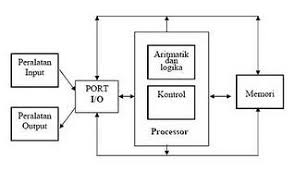
\includegraphics[width=1\textwidth]{figures/vonneumann}}
\caption{Skema Von Neumann}
\label{vonneumann}
\end{figure}
Arti dari istilah tersebut telah berevolusi untuk berarti komputer program tersimpan dimana pengambilan instruksi dan operasi data tidak dapat terjadi pada saat yang bersamaan karena mereka memiliki bus umum. Ini disebut sebagai bottleneck Von Neumann dan sering membatasi kinerja sistem \cite{markgrafneumann}.



%\chapter[Kernel]
%{Software\\ kernel}
%%Nama Kelompok: Kernel
%Kelas: D4 1B
%Anfhaz Grady Octavavian 1174048
%Dika Sukma Pradana 1174050
%Ikhsan Al Azis 1174049
%Rangga Putra 1174056
%Surya Pandu 1174036
%Syahriyan Zulfani 1174037
%Teddy Gideon Manik 1174038

	
	\section{Kernel}
	 Kernel adalah program komputer yang merupakan inti dari sistem operasi komputer, dengan kontrol penuh atas segala hal yang ada di sistem. Pada kebanyakan sistem, ini adalah salah satu program pertama yang dimuat
	 saat start-up (setelah bootloader). 
	 Ini menangani sisa start-up serta permintaan input / output dari perangkat lunak, menerjemahkannya ke dalam instruksi pengolahan data untuk unit pemrosesan pusat. Ini menangani memori dan periferal seperti keyboard, 
	 monitor, printer, dan speaker.
	 Kernel menghubungkan perangkat lunak aplikasi ke perangkat keras komputer.
	 Kode kritis kernel biasanya dimuat ke dalam area lindung memori, yang mencegahnya ditimpa oleh aplikasi atau komponen lain yang lebih kecil dari sistem operasi. Kernel menjalankan tugasnya, seperti menjalankan proses 
	 dan penanganan interupsi, di dalam ruang kernel. 
	 Sebaliknya, semua yang dilakukan pengguna ada di ruang pengguna: menulis teks di editor teks, menjalankan program di GUI, dll. Pemisahan ini mencegah data pengguna dan data kernel tidak saling mengganggu dan menyebabkan 
	 ketidakstabilan dan kelambatan. 
	 Antarmuka kernel adalah lapisan abstraksi tingkat rendah. Ketika sebuah proses membuat permintaan dari kernel, itu disebut system call. Desain kernel berbeda dalam cara mereka mengatur panggilan dan sumber sistem ini. 
	 Kernel monolitik menjalankan semua instruksi sistem operasi di ruang alamat yang sama untuk kecepatan. Sebuah mikrokernel menjalankan sebagian besar proses di ruang pengguna, untuk modularitas. contoh gambar kernel \ref{kernel}
	
\begin{figure}[ht]
	\centerline{\includegrapichs[width=1\textwidth]{figures/kernel.JPEG}}
	\caption{gambar dari kernel.}
	\label{kernel}
\end{figure}

		\subsection{Sejarah Kernel}
		 Kernel merupakan program komputer yang mengatur semua permintaan akan input/output dari perangkat lunak atau software.
		 Pada tahun 1990an, sebuah jenis algoritma pembelajaran baru dikembangkan, berdasarkan hasil teori pembelajaran statistik: Support Vector Machine (SVM). 
		 Hal ini memunculkan kelas baru secara teoritis SVM - kernel - untuk sejumlah tugas pembelajaran. 
		 Mesin kernel menyediakan kerangka kerja modular yang dapat disesuaikan dengan berbagai tugas dan domain dengan pilihan fungsi kernel dan algoritma dasar. 
		 Mereka mengganti jaringan syaraf tiruan di berbagai bidang, termasuk teknik, pencarian informasi, dan bioinformatika.
		 Belajar dengan Kernel memberikan pengenalan SVM dan metode kernel terkait. Meski buku ini diawali dengan dasar-dasar, namun juga mencakup penelitian terbaru. 
		 Ini menyediakan semua konsep yang diperlukan untuk memungkinkan pembaca menggunakan algoritma yang hebat yang telah dikembangkan melalui algoritma kernel dan untuk memahami dan menerapkan algoritma hebat yang telah dikembangkan selama beberapa tahun terakhir.
		 Sejarah Linux dimulai pada tahun 1991, ketika mahasiswa Universitas Helsinki, Finlandia bernama Linus Benedict Torvalds menulis Linux, sebuah Kernel untuk proses 80386
		 proses 32-bit pertama dalam kumpulan CPU intel yang cocok untuk PC.
		 Pada awal perkembangannya, sourche code Linux di sediakan secara bebas melalui internet. Kernel Linux berbeda dengan sistem Linux. Kernel Linux merupakan sebuah perangkat lunak.
		 Kernel Linux pertama kali yang dipublikasikan adalah versi 0.01, pada tanggal 14 Maret 1991. Sistem berkas yang didukung hanya sistem berkas Minix. Kernel pertama dibuat 
		 tanggal 14 Maret 1994 dan dikeluarkan versi 1.0, yang merupakan ujung tombak sejarah dari Linux. jenis ini adalah puncak dari tiga tahun perkembangan yang cepat dari kernel Linux. Fitur baru terbesar
		 yang disediakan adalah jaringan. Versi 1.0 mampu mendukung protokol standar jaringan TCP/IP. Kernel 1.0 juga memiliki sistem berkas yang lebih baik tanpa batasan-batasan sistem berkas Minix.
		 Setahun setelah versi 1.0, kernel 1.2 dirilis. Kernel versi 1.2 ini mendukung perangkat keras yang lebih luas. Pengembangan telah memperbarui networking stack untuk menyediakan
		 support bagi protokol IPX, dan membuat implementasi IP lebih lengkap dengan memberikan fungsi accounting dan firewalling. Kernel 1.2 ini merupakan kernel Linux terakhir yang hanya bisa di PC. 

		\subsection{Versi Kernel}
			\subsubsection{Monolithic}
			 Kernel Moonolithic memiliki seluruh servis dasar dari sistem operasi didalamnya. Kelebihan dari disain Monolithic adalah Efesiensi, sehingga performa sistem juga
			 meningkat. Monolithic juga memiliki kelemahan, salah satunya dalam hal stabilitas, dimana kemungkinan sistem crash lebih besar. Monolithic Kernel meliputi semua 
			 fungsi Kernel di satu modul. Monolithic kernel meliputi semua fungsi kernel di satu modul. Aplikasi dapat memanfaatkan fungsi kernel melalui sistem pemanggil. Alamat untuk kernel terpisah dari aplikasi untuk melindungi dari kekeliruan operasi aplikasi. Kernel menjadi sangat besar karena menyediakan beberapa fungsi untuk memuaskan permintaan user dan sekarang masalah mulai bermunculan;
			 1. Lemahnya Fleksibelitas
			 2. Modifikasi dari kernel memberi rekonfigurasi dan rekompilasi dari kernel dan pengulangan. Rekonfigurasi dan rekompilasi dari kernel memakan banyak waktu, dan operasi pengulangan tidak diinginkan untuk sistem non-stop.  
			 3. Portabilitas Rendah
			 4. Masuknya beberapa fungsi permintaan dan perbaikan pemanfaatan sistem, kode dari kernel menjadi sangat komplek.
			 5. Menyianyiakan Bar Alamat
			 6. Monolithic kernel termasuk beberapa fungsi dan sebagian dari mereka keluar dari penggunaan atau crash di beberapa aplikasi. Fungsi ini menyia-nyiakan bar alamat.
	
			\subsubsection{Microkernel}
			 Dalam ilmu komputer, mikrokernel (juga dikenal sebagai μ-kernel) adalah jumlah minimum perangkat lunak yang mendekati mekanisme yang dibutuhkan untuk mengimplementasikan sistem operasi (OS). Mekanisme ini mencakup pengelolaan ruang alamat tingkat rendah, manajemen benang, dan komunikasi antar proses (IPC).
			 Jika perangkat keras menyediakan beberapa cincin atau mode CPU, mikrokernel mungkin satu-satunya perangkat lunak yang dijalankan pada tingkat yang paling istimewa, yang umumnya disebut sebagai mode supervisor atau kernel. Fungsi sistem operasi tradisional, seperti driver perangkat, tumpukan protokol dan sistem berkas, biasanya dikeluarkan dari mikrokernel itu sendiri dan dijalankan di ruang pengguna.
			 Dari segi ukuran kode sumber, sebagai aturan umum, mikrokernel cenderung lebih kecil dari pada kernel monolitik. Mikrokernel MINIX 3, misalnya, memiliki sekitar 12.000 baris kode.

			\subsubsection{Hybrid Kernel}
			 Design Hybrid Kernel menyerupai Micokernel tetepi dengan tambahan kode yang menyebabkan Hybird Kernel dapat berjalan lebih cepat dari Micokernel. 
			 Di PAF Kernel, fitur tempat dianggap sebagai bagian intergal yang termasuk dalam predikat dan salah satu dari argumen nya. Kami mencatat dan yang lain disebut fitur 
			 Constituent Structure. Dua fitur ini memberikan informasi yang berbeda. Fitur Path mendeskripsikan informasi antara sebuah predikat dan argumen itu sementara fitur 
			 Constituent Structure menyimpan informasi tentang struktur syntax.
	
			\subsubsection{ExoKernel}
			 Exokernel adalah kernel sistem operasi yang dikembangkan oleh MIT Parallel dan Distributed Operating Systems group, dan juga merupakan kelas dari sistem operasi serupa.
			 Sistem operasi umumnya menyajikan sumber daya perangkat keras ke aplikasi melalui abstraksi tingkat tinggi seperti sistem file (virtual). Gagasan di balik exokernel adalah 
			 memaksa beberapa abstraksi mungkin pada pengembang aplikasi, memungkinkan mereka membuat keputusan sebanyak mungkin tentang abstraksi perangkat keras. Exokernel sangat kecil, 
			 karena fungsinya terbatas untuk memastikan perlindungan dan multiplexing sumber daya, yang jauh lebih sederhana daripada penerapan instruksi pelepasan pesan dan penerapan 
			 monolitik dari abstraksi tingkat tinggi secara mikrokernel konvensional.
			 Aplikasi yang diimplementasikan disebut sistem operasi perpustakaan; mereka mungkin meminta alamat memori tertentu, blok disk, dll. Kernel hanya memastikan bahwa sumber 
			 daya yang diminta bebas, dan aplikasi diizinkan untuk mengaksesnya. Akses perangkat keras tingkat rendah ini memungkinkan programmer untuk menerapkan abstraksi kustom, dan 
			 menghilangkan yang tidak perlu, yang paling umum untuk memperbaiki kinerja program. Hal ini juga memungkinkan pemrogram untuk memilih tingkat abstraksi yang mereka inginkan, tinggi, atau rendah.
			 Exokernel dapat dilihat sebagai penerapan prinsip end-to-end pada sistem operasi, karena aplikasi tersebut tidak memaksa program aplikasi untuk melapisi abstraksi di atas abstraksi 
			 lainnya yang dirancang dengan berbagai persyaratan.
			
			\subsubsection{Windows Kernel}
			 Akar Windows mencapai kembali ke akhir 1980-an. Kembali
			 Kemudian, banyak hal menarik terjadi di op-
			 Ruang desain sistem erating - termasuk SVR4, Mach
			 microkernel, inovasi dalam networking dan windowing sys-
			 tems, dan banyak proyek penelitian berbasis OS. Itu
			 keinginan untuk mendapatkan pengetahuan mendalam tentang pengembangan yang menarik ini-
			 ops memotivasi banyak siswa CS untuk belajar operasi
			 sistem saat itu. Dengan proyek OS kami, kami ingin membantu
			 Minat kembali minat pada sistem operasi lagi.
			 Dalam makalah ini, kami menganjurkan pendekatan langsung terhadap-
			 lingkungan pengajaran (dan pembelajaran) konsep OS. Kami menyajikan kami
			 pengalaman dari pengajaran program OS berbasis Windows dur-
			 dalam sepuluh tahun terakhir ini. Kami menyarankan skema tiga fasa,
			 dimana siswa pertama belajar menguasai
			 kamu
			 sistem ser-mode di-
			 Koraces (U) - sering disebut sebagai "pemrograman sistem".
			 Kedua, mereka perlu menguasai prinsip dan alat untuk mon-
			 itor dan perilaku OS easure (M). Dan ketiga, siswa
			 harus disajikan dengan rincian pelaksanaan utama OS
			 kernel (K). Mengikuti Pendekatan UMK , bahkan com-
			 proyek yang rumit seperti modifikasi pelaksanaan
			 manajemen memori di dalam kernel Windows bisa jadi mobil-
			 mengikuti kurikulum OS sarjana. Undertakings,
			 seperti proyek Manajemen Memori Abstrak (AMM)
			 mengintegrasikan dengan baik dengan courseware kami yang telah dikembangkan sebelumnya -
			 Kit Sumber Daya Kurikulum Microsoft Windows Internals(CRK).
			 Microsoft membuat source kernel Windows secara luas memanfaatkan-
			 mampu akademisi di tahun 2006 , menggantikan yang sebelumnya terbatas
			 distribusi yang tersedia hanya untuk memilih universitas.
			 Sejak itu, kami telah memperluas penggunaan Windows sebelumnya
			 dalam kursus OS dengan mengembangkan sejumlah proyek dan laboratorium
			 yang mengandalkan modifikasi kernel Windows. Proyek ini
			 fokus pada topik seperti penjadwalan / pengiriman, sinkronisasi-
			 dan pengelolaan memori. Dalam tulisan ini, kita
			 Hadirkan Manajemen Memori Abstrak (AMM)
			 yang terdiri dari bagian U, di mana siswa prac-
			 API sistem yang relevan (seperti fungsi Windows API
			 VirtualAllocEx, bagian M, dimana kita bertanya kepada siswa
			 untuk membiasakan diri dengan teknik pengukuran dan
			 alat (seperti monitor kinerja Windows - perf-mon.exe), dan bagian K	dimana siswa perlu memodifikasi
			 kode sumber (mis., ntos / mm / wsmanage.c), kompilasi, dan jalankan
			 versi Windows mereka sendiri. Selama kursus, proyek
			 ditugaskan ke kelompok tiga siswa.
			 Dalam sisa makalah ini, pertama-tama kami menyajikan ikhtisar 490
			 tentang proyek yang kami buat untuk WRK. Lalu, kami hadir
			 bagian kernel (K) dan pengukuran (M) dari AMM
			 proyek. (Kami telah menghilangkan bagian mode pengguna (U) karena
			 keterbatasan ruang). Sebaliknya, kami menyajikan umpan balik dari stu-
			 penyok yang mengambil kursus kami Akhirnya, kita menyimpulkan makalahnya
			 dengan prospek proyek UMK masa depan.
			 Untuk mencegah aplikasinya
			 ion untuk menyimpan duplikat dari
			 konten yang dilindungi, Windows Kernel Hook digunakan untuk mengubah
			 perilaku /"Save/" oleh modi
			 memamerkan fungsi yang sesuai
			 alamat. Akibatnya, aplikasi tidak bisa menyelesaikan ini
			 operasi berhasil dan tidak duplicate benar-benar diselamatkan.
			 Melalui penelitian, kami menentukan
			 sesuatu fungsi kernel kunci masuk	
			 Proses menabung duplikat, yaitu /"ZwWriteFile/" yang mana bertanggung jawab untuk mengoperasikan tugas menulis. Dengan memuat NT Sopir, kita bisa menimpa alamat ZwWriteFile fungsi di SSDT dengan alamat fungsi kait
			 NewZwWriteFile). Dalam keadaan seperti ini, NewZwWriteFile akan dipanggil kapan sistem bermaksud untuk memanggil ZwWriteFile. Di NewZwWriteFile , kita bisa memanggil fungsi aslinya ZwWriteFile
			 dengan dimodifikasi parameter dan run re nya sults akan dikembalikan ke NewZwWriteFile, sehingga yang terakhir bisa menutupi kegagalan panggilan.
	
		\subsection{Kernel Linux}
		 Kernel Linux adalah salah satu proyek open-source yang paling menarik namun paling tidak dipahami. Ini juga merupakan dasar untuk mengembangkan kode kernel baru. 
		 Itulah sebabnya Sams sangat antusias untuk membawa Anda informasi pengembangan kernel Linux terbaru dari orang dalam Novell di edisi kedua Pengembangan Kernel Linux. 
		 Panduan praktis dan otoritatif ini akan membantu Anda lebih memahami kernel Linux melalui cakupan terkini dari semua subsistem utama, fitur baru yang terkait dengan kernel Linux 2.6 dan informasi orang dalam mengenai perkembangan yang belum pernah dirilis. 
		 Anda dapat melihat kernel Linux secara mendalam dari sudut pandang teoritis dan penerapan saat Anda membahas berbagai topik, termasuk algoritme, antarmuka panggilan sistem, strategi paging dan sinkronisasi kernel. 
		 Dapatkan informasi terbaik dari sumber di Linux Kernel Development.
	
		\subsection{Kernel Android}
		 Pertama-tama, kernel Linux perlu dikompilasi
		 sesuai dengan perangkat kerasnya. File konfigurasi
		 (file defconfig / .config) harus dimodifikasi agar sesuai dengan teknis
		 spesifikasi perangkat keras Spesifikasi perangkat keras
		 perangkat keras dapat ditentukan dengan menggunakan alat yang tersedia
		 jaring (misalnya Database WURFL, yang merupakan singkatan dari Wireless
		 File Sumber Universal).
		 Ini memastikan bahwa versi kernel tertentu akan
		 jalankan pada hardware dan support File System yang ada
		 telah dibangun untuk perangkat keras.
		 Setelah kita memiliki file konfigurasi yang benar, kernel perlu 
		 ditambal untuk mendukung perangkat keras. Jika kernelnya adalah
		 dari pohon kernel Linux, perlu ditambal untuk mendukungnya
		 Android juga. Jika kernelnya adalah kernel Android, tambalan hanya untuk
		 mendukung Platform perlu diterapkan.
		 Patch membuat kernel yang kompatibel dengan Android dan platform
		 
\cite{engler1995exokernel}
\cite{liedtke1996toward}
\cite{che2006hybrid}
\cite{kashiwagi1996design}
\cite{schmidt2010teaching}
\cite{wang2009usage}
\cite{lee2003firm}

\chapter[Perintah DOS dan UNIX]
{Software\\ DOS dan UNIX}
%M. A. Faris 1174041
%Evietania Charis Sujadi 1174051
%Iqbal Panggabean 1174063
%Hagan Rowlenstino 1174040
%Irvan Rizkiansyah 1174043
%Kelas D4 TI 1B
%Kelmopok 5


	\section{Perintah pada Unix}
		\subsection{Definisi}
		\hspace*{1cm}Perintah pada UNIX merupakan perintah yang dijalankan pada sistem operasi UNIX, yang diberikan user untuk melakukan perintah yang diinginkan baik berupa perintah/command internal, ataupun perintah eksekusi suatu file program yang biasa disebut perintah/command eksternal. Program penterjemah perintah/command yang menjembati antara user dengan sistem operasi dalam hal ini kernel yaitu shell. Shell dapat digunakkan user untuk menyusun perintah pada beberapa file untuk dieksekusi sebagai sebuah program. Shell pada UNIX tidak hanya menyediakan 1 atau 2 shell saja, namun dilengkapi oleh banyak shell dengan kumpulan perintah yang sangat banyak, sehingga user dapat memilih shell mana yang lebih mudah dalam membantu menyelesaikan pekerjaannya, dan dapat berpindah pindah dengan mudah dari shell satu ke shell yang lainnya.Ini adalah contoh beberapa command UNIX pada gambar \ref{command}.
		
		\begin{figure}[ht]
			\centerline{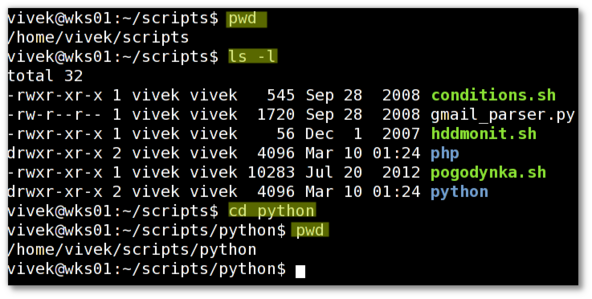
\includegraphics[width=0.5\textwidth]{figures/command.png}}
			\caption{Contoh command UNIX}
			\label{command}
			\end{figure}
		
		\subsection{Sejarah}
		\hspace*{1cm}UNIX adarah sistem operasi yang cepat dan kuat, karena dapat menampung banyak user sekaligus dan juga ideal untuk penyedialayanan internet.banyak ilmuan komputer yang berkata bahwa UNIX lebih baik dari windows karena lebih banyak fungsi dan dapat berkreasi di komputer lebih dalam. UNIX adalah sistem operasi yang paling banyak digunakan untuk server internet. UNIX dibuat pada tahun 1969, Versi awal dari UNIX file sistem terbuat dari hasil sketsa desain sebuah file sistem yang dikembangkan oleh Ken Thompson, Dennis Ritchie dan yang lainnya yang tergabung dalam General Electric Company and Project MAC of the Massachusetts Institute of Technology. Thompson dan Ritchie meng-implementasikan sistem mereka pada komputer PDP-7, termasuk versi awal UNIX file sistem, proses sub-sistem, dan beberapa set kecil dari utility programs, dan dan terlahirlah sistem baru yang dinamakan UNIX. Ritchie mengembangkan Bahasa Pemrograman B yang dihasilkan oleh Thompson menjadi satu yang dinamakan Bahasa Pemrograman C. lalu didistribusikan ke mahasiswa pada tahun 1970. Saat itu Amerika sedaang dalam perang dingin dan membutuhkan sistem komunikasi yang tahan dari ledakan nuklir. pada saat itu mreka masih menggunakan jaringan yang terpusat, jadi jika diserang dapat langsung tidak berfungsi. Mreka pun berfikir untuk menyambungkan setiap stasiun jaringan, jadi jika yang satu tidak berfungsi, masih ada yang lain. Pada saat itu mreka masih belum punya sistem operasi, mereka pun memilih UNIX dan jadilah Advanced Reseacrh Project Network atau yang kita kenal sebagai ARPANet.Setiap perusahaan besar pun punya UNIX versi mreka sendiri dikarenakan internet dijalankan oleh sistem operasi UNIX hal ini terjadi pada sekitar tahun 1978-1998. UNIX mendapatkan keuntungan karena merupakan pelopor pertama internet dan telah banyak digunakan. UNIX juga menunjukan beberapa efek dari jaringannya karena  seiring bertambahnya angka pengguna UNIX, bertambah pula program-program yang dibuat untuk para pengguna, dan banyak juga program yang dapat di unduh gratis. Para pengguna UNIX pun terus berkembang karena setiap ad bug, komunitas pengguna akan berusaha untuk membetulkannya. Lalu pasar sistem preasi pun mulai berbalik. Bill Gates membuat sistem operasinya sendiri yaitu DOS, lalu Apple pun mengeluarkan sistem operasi bikinannya sendiri yang menyatu dengan hardwarenya dan mempunyai graphic interface yang bagus. Lalu pasar mejadi lebih berbalik karena Bill Gates melisensi graphic interface nya Apple dan mengembangkan sistem operasi baru bernama windows. Sekarang, UNIX hanya dugunakan di tempat kerja saja. Walaupun UNIX adalah sistem operasi yang kuat, digunakan untuk banyak penelitian, membuat special effect untuk industri film, dan unggul dalam jaringan karena adalah sistem operasi yang digunakan untuk menjalankan internet juga untuk intranet, tetapi hal yang sangat krusial adalah banyak orang yang berfikir bahwa sistem operasi ini tidak user-friendly. Karena UNIX lebih fokus kepada fungsionalnya, tidak seperti Apple yang tefokus kepada grafis dan Microsoft yang terfokus kepada interaksi yang memudahkan pengguna. Disinilah kelemahan UNIX, mereka sudah tertinggal jauh sejak yang lain menggunakan graphic user interface dan sekarang kebanyak orang lebih memilih windows. walaupun UNIX dapat di unduh gratis tetapi hanya sedikit orang yang mau belajar dan menggunakannya, karena harus belajar sendiri tanpa di bimbing, dan juga sekarang tidak ada komputer atau laptop baru yang terinstall UNIX, karena mreka lebih memilih windows. Alasan utama lainnya adalah karna belum ada versi standard dari UNIX itu sendiri. Sebenarnya banyak versi UNIX dari sejak pengembangannya, tetapi sebenarnya ada dua versi utama, yang menyebabkan konflik para user. ATdanT adalah perusahaan pertama yang merilis UNIX untuk komunitas akademik tanpa menuntut biaya, tetapi saat UNIX mulai populer. pada tahun 1978, ATdanT mulai mengenakan biaya pada pengguna UNIX. Para mahasiswa Berkley menentang nya dan membuat versi mreka sendiri dan menamakannya BSD UNIX (Berkley Software Distribution). jadi UNIX mempunyai dua versi utama, yaitu versi ATdanT dan versi Sys V atau BSD. Kedua versi ini susah untuk dibedakan kecuali anda adalah programmer.
	
		\subsection{Versi}
		\begin{itemize}
			\item 1969 - UNIX pada PDP-7
			\item 1971 - UNIX Versi 1, pada DEC PDP-11/20
			\item 1973 - UNIX Versi 4, sudah menggunakan Bahasa Pemrograman C
			\item 1974 - UNIX Versi 5, untuk pendidikan
			\item 1975 - UNIX Versi 6, mulai timbul versi BSD
			\item 1979 - UNIX Versi 7, Portable dan dilengkapi kompiler dan Bourne Shell
			\item 1982 - UNIX System 3
			\item 1983 - UNIX System 5, ditambahkan versi BSD seperti vi dan c shell
			\item 1988 - UNIX System 5 Release 4, membuat semua program yang ditulis untuk System V dan Berkeley UNIX menjadi kompatibel dalam satu sistem.
		\end{itemize}
			\begin{figure}[ht]
			\centerline{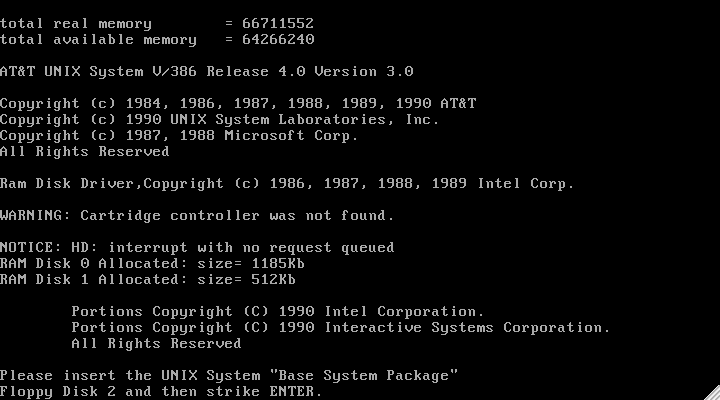
\includegraphics[width=1\textwidth]{figures/UNIXSVR4.png}}
			\caption{UNIX System V Release 4}
			\label{UNIXSVR4}
			\end{figure}
		Ini adalah contoh UNIX Versi 4 Release 4 \ref{UNIXSVR4}
		
		\subsection{Contoh}
		\begin{itemize}
			\item pwd : perintah ini artinya \"print working directory\" digunakan untuk mengetahui di direktori mana kita sedang berada.
			\item cd : perintah ini artinya \"change directory\" digunakan untuk berganti atau berpindah direktori.
			\item ls : perintah ini artinya \"list\" digunakan untuk melihat semua file dan folder dalam direktori dimana kita sedang berada.
			\item mkdir : perintah ini artinya \"make directory\" digunakan untuk membuat direktori atau folder baru.
			\item rmdir : perintah ini artinya \"remove directoy\" digunakan untuk menghapus direktori atau folder.
			\item clear : perintah ini digunakan untuk menghapus semua tampilan yang ada pada layar terminal.
			\item su : perintah ini digunakan untuk mengubah hak akses user menjadi root.
			\item ifconfig : perintah ini digunakan untuk melihat konfigurasi IP yang ada di network interface yang ada dalam PC kita.
			\item cp : perintah ini digunakan untuk membuat salinan dari sebuah file.
			\item mv : perintah ini digunakan untuk memindahkan suatu file dari direktori ke direktori lainnya.
		\end{itemize}
			\begin{figure}[ht]
			\centerline{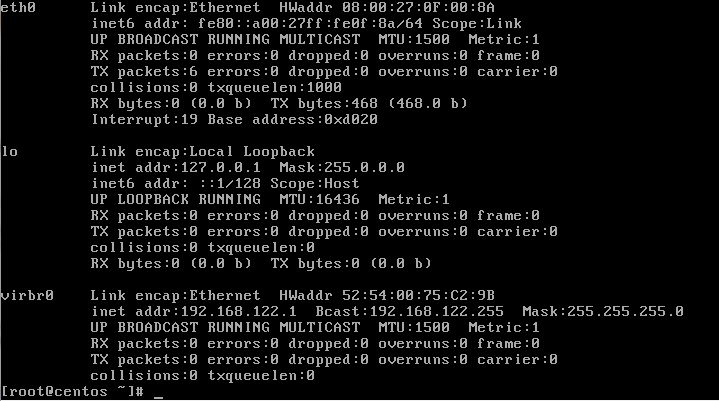
\includegraphics[width=1\textwidth]{figures/ifconfig.png}}
			\caption{Perintah untuk mengecek Network Interface}
			\label{ifconfig}
			\end{figure}
			
			\begin{figure}[ht]
			\centerline{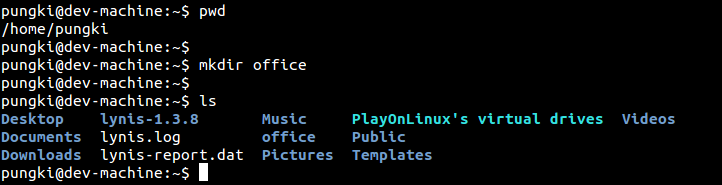
\includegraphics[width=1\textwidth]{figures/mkdir.png}}
			\caption{Perintah untuk membuat folder}
			\label{mkdir}
			\end{figure}
		Dibawah ini adalah contoh perintah ifconfig \ref{ifconfig}
		Dibawah ini adalah contoh perintah mkdir \ref{mkdir}
		
\pagebreak
	
	\section{Perintah Pada DOS}
		\subsection{Definisi}
		\hspace{1cm}Perintah pada DOS merupakan perintah atau command yang dapat dijalankan pada sistem operasi DOS. terdapat 2 jenis perintah dalam DOS, yaitu perintah internal, yaitu perintah yang sudah ada dalam COMMAND.COM (interpreter perintah DOS), dapat langsung di eksekusi oleh kernel DOS, seperti: Date, Time, Copy, atau juga Del. sedangkan perintah eksternal, yaitu perintah yg tidak ada dalam COMMAND.COM, dan memerlukan sebuah file yang dapat dieksekusi dan terdapat didalam direktori aktif, Seperti: fdisk, format, ataupun edit.
		
		\vspace{1cm} Ini adalah contoh perintah - perintah yang dilakukan pada DOS 
		\ref{commanddos}
		\begin{figure}[ht]
			\centerline{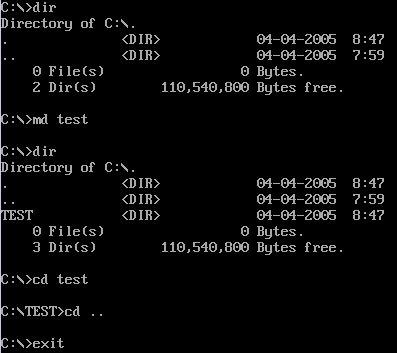
\includegraphics[width=0.5\textwidth]{figures/commanddos.png}}
			\caption{Perintah Pada DOS}
			\label{commanddos}
			\end{figure}
			
		\subsection{Sejarah}
		\hspace{1cm}Pada pertengahan tahun 1980, Tim Paterson membuat sistem operasi yang dinamakan 86-DOS, yang merupakan cikal bakal MS-DOS. Pada tahun 1981, Microsoft membeli hak cipta 86-DOS, membuat perubahan besar, dan mengubah namanya menjadi MS-DOS. MS-DOS pertama kali digunakan pada PC-DOS 1.0 yang dikeluarkan pertama kali oleh IBM dan menjadi PC pertama yang dibuat oleh IBM pada musim gugur tahun 1981. Pada tahun 1982 bulan juni IBM merilis MS-DOS 1.25 untuk memperbaiki beberapa bug dan agar bisa mendukung double-sided disks dan meningkatkan independesi hardware di kernel DOS. Versi ini dikeluarkan jg oleh beberapa vendor selain IBM, seperti COMPAQ, Columbia, dan yang lainnya, MS-DOS versi 1.0 pun tidak lagi digunakan. MS-DOS versi 2.0 pun dirilis pada bulan maret tahun 1983, dan mengalami banyak peningkatan dari versi sebelumnya, seperti mendukung disket yang memiliki kapasitas besar, mendukung penggunaan shell, dan yang lainnya. tidak lama kemudia keluar MS-DOS 2.11 untuk meningkatkan kualitas penggunaan seperti 16-bit huruf kanji, dan beberapa bugs. MS-DOS versi 2.25, rilis pada bulan oktober tahun 1985 yang di distribusi ke bagian timur dan tidak pernah rilis di eropa dan United States. MS-DOS 3.0 di keluarkan oleh IBM pada bulan agustus tahun 1984 yang menambahkan fitur baru seperti penambahan format mata uang dunia, meluaskan pelaporan error dan yang lainnya. MS-DOS versi 4 pun di rilis pada tahun 1988 dengan meningkatkan visual shell dan mendukung file sistem yang lebih besar. Selama MS-DOS mengalami peningkatan, Microsoft dengan berusaha membuat sistem operasi yang menggunakan user interface dan multitasking, dan terlahirlah Microsoft Windows.
		\vspace{1cm} Ini adalah contoh MS-DOS Versi 3.0 \ref{win31}
		\begin{figure}[ht]
			\centerline{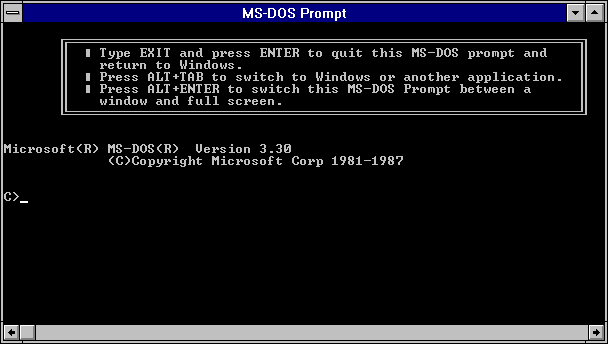
\includegraphics[width=0.5\textwidth]{figures/win31.png}}
			\caption{MS-DOS Versi 3.0}
			\label{win31}
			\end{figure}
		
		\subsection{Versi}
		\begin{itemize}
			\item MS-DOS 1.0 - 1981, Sistem operasi pertama pada IBM PC
			\item MS-DOS 1.1 - Lebih banyak di distribusikan oleh OEMS dibandingkan IBM
			\item MS-DOS 1.25 - Perbaikan beberapa bugs
			\item MS-DOS 2.0 - Struktur file dan ditambahkan hard-disk
			\item MS-DOS 2.01 - Dikenalkan dengan PCjr
			\item MS-DOS 2.11 - Perbaikan beberapa bug di MS-DOS Versi 2.01
			\item MS-DOS 3.0 - ditambahkan hard disk yang lebih besar
			\item MS-DOS 3.1 - Mendukung Jaringan Microsoft
			\item MS-DOS 3.2 - Mendukung disk ukuran 3.5 inch
			\item MS-DOS 4.0 - Mendukung logical volume lebih besar dari 32 MB, visual shell
		\end {itemize}
		
		\vspace{1cm} Ini adalah contoh MS-DOS Versi 4.0 \ref{dosv4}
		\begin{figure}[ht]
			\centerline{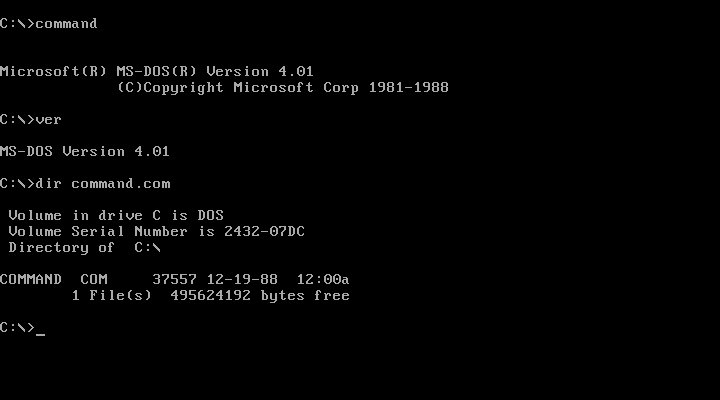
\includegraphics[width=0.5\textwidth]{figures/dosv4.png}}
			\caption{MS-DOS Versi 4.0}
			\label{dosv4}
			\end{figure}
		
		\subsection{Contoh}
		\begin{itemize}
			\item Chdir / CD : yang artinya \"change directory\" untuk berpindah direktori
			\item CLS : yang artinya \"clear screen\" untuk menghapus atau mengosongkan semua teks yang ada di layar
			\item Del : yang artinya \"delete\" untuk menghapus file atau beberapa file yang dinyatakan
			\item Mkdir / MD : yang artinya \"make directory\" untuk membuat suatu direktori atau folder
			\item Prompt : digunakan untuk mengubha prompt yang di gunakan di MS-DOS
			\item Time : digunakan untuk menampilkan atau mengatur jam pada sistem
			\item CD.. : digunakan untuk kemabali 1 level direktori di atasnya
			\item Vol : yang artinya \"volume\" untuk menampilkan label pada drive tertentu dan serial numbernya
			\item Ver : yang artinya \"versi\" untuk menampilkan versi dari dos yang dipakai
			\item Tree : untuk menampilkan direktori dengan semua direktori yang terdapat didalamnya dengan bentuh diagram (pohon)
			\item Deltree : untuk menghapus direktori beserta seluruh isinya
		\end{itemize}
		Ini adalah contoh perintah date pada DOS \ref{date}
		Ini adalah contoh perintah dir pada DOS \ref{dir}
			\begin{figure}[ht]
			\centerline{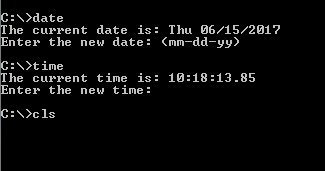
\includegraphics[width=0.5\textwidth]{figures/date.png}}
			\caption{Perintah untuk melihat dan mengatur jam dan tanggal}
			\label{date}
			\end{figure}
			
			\begin{figure}[ht]
			\centerline{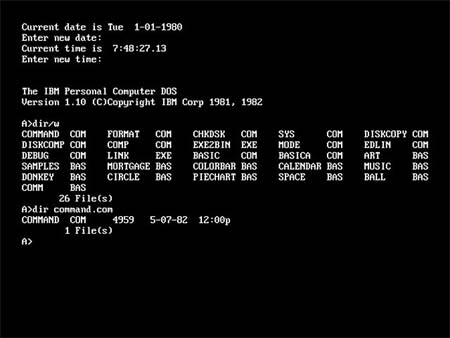
\includegraphics[width=0.5\textwidth]{figures/dir.jpg}}
			\caption{Perintah untuk melihat daftar file di direktoris}
			\label{dir}
			\end{figure}
			
\newpage

	\vspace*{1,5cm}Artikel yang dirangkum dari sebuah buku yang berjudul The design of the UNIX operating system \cite{bach1986design}.
		
	\vspace*{1cm}Artikel The UNIX System: The Evolution of the UNIX TIme-sharing System \cite{ritchie1984unix}.
	
	\vspace*{1cm}Artikel yang dirangkum dari sebuah buku yang berjudul UNIX: Teknik Penguasaan Secara Sistematis \cite{setiawanunix}
	
	\vspace*{1cm}Artikelyang dirangkum dari sebuah buku yang berjudul Advanced MS-DOS Programming \cite{duncan1988advanced}.
	

	\section{Coaxial}
		\subsection{Definisi}
		\hspace*{1cm}Kabel coaxial terbagi menjadi dua jenis yang berbeda, yaitu thick coaxial cable (diameternya agak besar) lalu ada juga thin coaxial cable (berdiameter lebih kecil). Thick coaxial cable sudah dispesifikasikan dengan berdasarkan standar IEEE 802.3 10BASE5, yang rata-rata diameternya adalah sekitar 12cm, yang biasanya diberikan warna kuning. Kabel ini juga biasa disebut dengan standard ethernet atau juga bisa dipanggil dengan thick Ethernet, atau yang biasa dikenal dengan ThickNet dan yellow cable. kabel jenis ini mempunyai spesifikasi dan aturan sebagai berikut :
		\begin{itemsize}
			\item Setiap ujungnya harus diterminasi menggunakan terminator rakitan sebesar 50-ohm.
			\item Peralatan yang terhubung maksimal 3 segment.
			\item Ada pemancar tambahan di setiap pemancar jaringannya.
			\item Setiap segment tadi maksimal berisi 100 perangkat jaringan, sudah termasuk juga repreater.
			\item Untuk kabelnya, maksimum sekitar 500 meter per segment nya.
			\item Jarak antar segment tidak boleh lebih dari 1500 meter.
			\item Ground harus sudah terpasang di setiap segment.
			\item Jarak terjauh untuk pencabang dari kabel utama ke device hanya sekitaran 5 meter saja.
			\item Setiap pencabang paling banyak hanya boleh berjarak sekitar 2,5 meter.
		\end{itemsize}
		\hspace{0cm}Yang kedua adalah thin coaxial cable. Kabel koaxial tipis ini biasa digunakan untuk transciver di banyak radio amatir yang hanya memerlukan output atau pengeluaran daya yang kecil. Agar dapat digunakan sebagai jaringan, kabel ini harus memenuhi standar IEEE 802.3 10BASE2,yang diameter rata-ratanya kurang lebih 5mm dengan warna hitam atau warna gelap yang lain dan setiap perangkat di sambungkan ke BNCT-connector. Jika ingin kabel ini diimplementaasikan dengan T-Connector dan terminator di dalam sebuah jaringan, maka harus mengikuti aturan-aturan ini: 
		\begin{itemsize}
			\item Seperti biasa, tiap ujungnya diberikan terminator sebesar 50-ohm.
			\item Panjang kabel per segment nya kira-kira 185 meter.
			\item Maksimal dapat terkoneksi 30 device per segment.
			\item Kartu jaringannya dapat menggunakan transceiver yang sudah terpasang, kecuali untuk reapreater.
			\item Maksimal 3 segment yang berhubungan satu dengan yang lainnya.
			\item Sebaiknya menggunakan satu ground di setiap segment nya.
			\item Panjang minimal T-connector minimal 0,5 meter.
			\item Panjang maksimum kabel per segment adalah 555 meter.
			\item dapat menampung maksimum 30 device per segmentnya.
		\end{itemsize}
		

\chapter[Windows]
{Software\\ windows}
% Nama Kelompok: Kelompok 1
% Kelas: D4 TI 1A
% Anggota: 1. Dezha Aidil Martha 1174025
% 		   2. Habib Abdul Rasyid 1174002
% 		   3. Muhammad Tomy Nur Maulidy 1174031
% 		   4. Nico Ekklesia Sembiring 1174095
% 		   5. Felix Setiawan Lase 1174026
% 		   6. Damara Benedikta Siolemba 1174012

\section{Sejarah Windows}
	pada awal mulanya windows muncul dengan nama QDOS (Quick and Dirty Operating System) yang ditulis oleh Paterson dari Seatle Computer pada tahun 1980.
Kemudian pada tahun 1981 Bill gates dari microsoft membeli licensi QDOS tersebut dan mengganti namanya menjadi MS-DOS seiring perkembangan dari tahun ke tahun namanya berubah menjadi Windows seperti yang kita ketahui sekarang ini.
\subsection{kelebihan windows}
	1.	sistem operasi yang user friendly
	2.	dukungan hardware yang lengkap
	3.	mendukung sistem berkas dengan format FAT,FAT16,FAT32, NTFS dan ISO
\subsubsection{Kekurangan}
	1.	rentan terkena virus
	2.	harga licensi yang cukup tinggi
	3.	tidak ada efek 3D dan resolusi gambar yang rendah.


\section{Macam - macam Windows dan penjelasannya}

% Windows 3.1 
\subsection{Sejarah Windows 3.1}
\ref{Windows31}
	Windows 3.1 memiliki sistem operasi 16 bit, diproduksi oleh microsoft untur client, pertama kali dikeluarkan pada 6 April 1992 sebagai versi lanjutan dari Windows 3.0 \cite{brodsky1996just}
	\subsubsection{Karakteristik Windows 3.1}
		1.Dirilis pada tanggal 6 April 1992
		2.Mendukung software multimedia
		3.Menggunakan mkernel hibrida
		4.Diperkenalkan sistem berkas NTFS
	\subsubsection{Sistem keamanan Windows 3.1}
		1.Keamanan masih kurang bagus
		2.Tidak ada pembatasan user untuk menggunakan OS
		3.Rentan terhadap virus
	\subsubsection{Kelebihan Windows 3.1}
		1.Memudahkan komunikasi antar anggota workgroup
		2.Dukungan driver yang lebih banyak
		3.Lebih mudah mengakses file dan aplikasi di komputer lain
		4.Administrasi sistem jaringan relatif lebih mudah
	\subsubsection{Kekurangan}
		1.Virus gampang menyerang OS
		2.Sering terjadi maintenence, tetapi masih belum mengatasi virus
		3.Sistem nya kurang stabil

\begin{figure}[ht]
\centerline{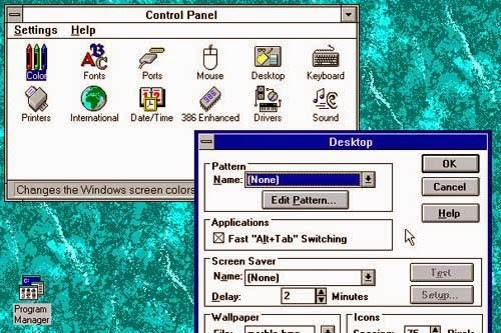
\includegraphics[width=1\textwidth]{figures/Windows31.JPG}}
\caption{tampilan desktop di windows 3.1}
\label{Windows31}
\end{figure}

% Windows 95
\section{windows 95}
\ref{desktop95}
	Windows 95 merukapan sistem operasi hubruda 16-bit/32-biit dan 
	diproduksi oleh microsoft, windows ini di perkenalkan kepada 
	publik pada tanggal 14 agustus 1995. Windows 95 ini adalah produk 
	pertama windows dengan kernel monolotic yg berjalan  -/+  60 tanpa dos 
	dan di dalamnya sudah berisi microsoft office 1995. \cite{petzold1996programming} 
	\subsection{Lima versi windows 95}
		1.windows 95
		2.windows 95 A
		3.windows 95 B
		4.windows 95 B USB
		5.windows 95 C


\begin{figure}[ht]
\centerline{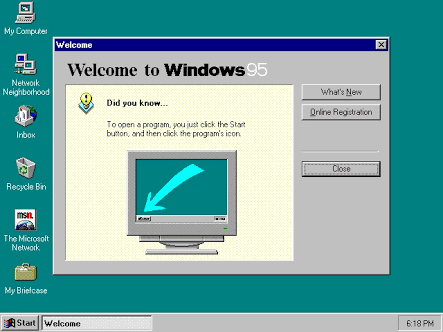
\includegraphics[width=1\textwidth]{figures/desktop95.PNG}}
\caption{tampilan desktop di windows 95.}
\label{desktop95}
\end{figure}

% Windows 98
\section{windows98}
		\ref{Desktopwindows98}
	windows 98 adalah pengembangan dari windows 95 dimana windows 98 diluncurkan agar lebih stabil daripada versi sebelumnya, windows versi 98 ini adalah versi pertama yang dibuat secara spesifik untuk konsumen. pada windows 98 ini memiliki fitur menarik yang disebut \"Deskbar\" fitur ini bisa mengunduh bilah alat desktop(deskbar) dari situs-situs favorit mereka.
	Dalam sebuah artikel dari davis menyebutkan bahwa revisi dari windows 98 adalah pemasangan dan perubahan antarmuka hingga komponen built-in, perangkat tambahan dan multimedia baru dan bagian referensi teknis yang jauh kebih luas. \cite{Davis:1998:W9B:551711}
	\subsection{fitur tambahan dari windows 98}
			Pada windows 98 ini mencakup banyak driver dan dukungan berkas system FAT32.
		Dalam sebuah artikel dari mcfedries menyebutkan bahwa windows 98 memiliki fitur windows terbaru, anda dapat menemukan Internet Explorer 4.0 dan Active Desktop; mengatur Outlook Express untuk surat internet dan surat CompuServer; Instalasi,konfigurasi, dan kostumisasi windows 98 termasuk dua-boot; membuka potensi multimedia windows 98 \cite{mcfedries1998windows}

		\begin{figure}[ht]
		\centerline{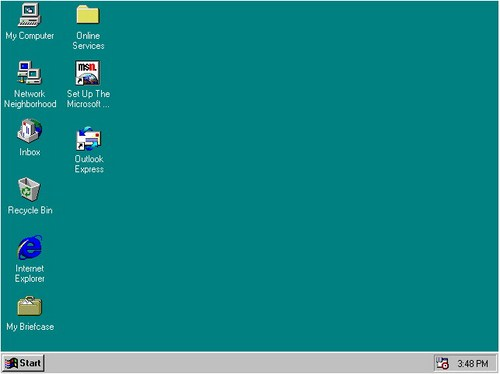
\includegraphics[wiedth=1\textwidth]{figures/Desktopwindows98.JPG}}
		\caption{tampilan desktop windows 98}
		\label{Desktopwindows98}
		\end{figure}

% Windows 2000
\section{windows2000}
	Windows 2000 diluncurkan oleh perusahaan multinasional Microsoft Corporation pada tanggal 17 Februari 2000 di Washington, Amerika Serikat. 
	Dalam sebuah buku yang ditulis oleh Solomon disebutkan bahwa Windows 2000 merupakan flatform dari sistem operasi generasi lanjutan dari windows seri NT4.0 dan menyediakan fitur-fitur lebih tinggi,ekstensi aritmatika yang lebih kuat dan akurat, memiliki instruksi khusus untuk multimedia, serta mendapat dukungan memori yang besar dari chip Intel 64-bit dengan fitur multiprocessing yang luas \cite{solomon2000inside}
	\subsection{tujuan perancangan windows 2000}
		Pada awal pembuatannya, Windows 2000 dirancang untuk memenuhi kebutuhan akan bisnis yang dilakukan melalui dunia maya seperti e-commerce, data dari suatu tempat, proses transaksi online, dan aplikasi yang memiliki performa tinggi.
	\subsection{fokus pengembangan windows 2000}
		Fokus pengembangan Windows 2000 terdapat pada bidang keandalan sistem dan diharapkan sistem operasi baru yang diluncurkan pada saat itu lebih dapat diandalkan dari sistem operasi yang lain.
		Dalam artikel yang ditulis oleh Murphy, tidak adanya standar industri yang ditujukan untuk mengkarakterisasi keandalan sistem menuntut Microsoft agar menambahkan fungsionalitas kerja kedalam sistem operasinya agar lebih dapat diandalkan dan mengurangi persepsi pelanggan mengenai terjadinya bug dan masalah yang akan terjadi dalam penggunaan fungsi dan fitur-fitur baru dasi sistem operasi yang baru ini. Sehingga pelangga akan merasa nyaman dalam menggunakan sistem operasi yang baru ini \cite{murphy2000windows} 

% Windows 2003 server
\section{windows 2003 server}
\ref{windows2003server}
	windows 2003 adalah pembaruan dari windows 2000 server yang menggabungkan kompatibilitas dan fitur-fitur lainnya dari windows XP, alasan windows 2003 ini menggunakan metode kompatibilitas agar aplikasi lama dapat bekerja dengan stabiLitas yang besar, semua itu dibuat kompatibel dengan jaringan yang berbasis windows NT 4.0 . pada windows 2003 ini menawarkan berbagai fitur keamanan baru, seperti \"Manage Your Wizard\".
	dalam sebuah artikel yang ditulis oleh Litch Field menyebutkan bahwa windows 2003 dirancang agar aman diluar kontak. Sebagian dari keamanan diadopsi oleh microsoft untuk versi windows terbaru dengan tujuan mengurangi resiko yang ditimbulan oleh kerentangan buffer offerflow \cite{litchfield2003defeating}
	\subsection{edisi windows server 2003}
		windows server 2003 menggunakan kernel windows NT versi 5.2 
		windows server 2003 tersedia dalam lima buah edisi:
		1.windows server 2003 standart edition
 		2.windows server enterprise edition (32bit dan 64bit)
		3.windows server datacenter edition
		4.windows server small business server
		5.windows strorage server 2003


\begin{figure}[ht]
\centerline{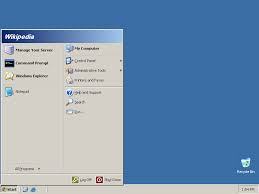
\includegraphics[width=1\textwidth]{figures/windows2003server.JPG}}
\caption{tampilan desktop di windows 2003 server}
\label{windows2003server}
\end{figure}
% Windows XP
	\section{Windows XP}
		Windows XP dirilis setelah Windows 2000 dan Windows Me (millenium edition), Windows XP sebelumnya dikenal dengan sebutan sandi Whistler. Dan pertama kali dipublikasikan tanggal 25oktober 2001. Windows XP adalah kependekan dari Windows Experience yang artinys pengalaman. Windows XP mempunyai daya tarik tersendiri karena Windows XP merupakan Windows pertama yang dibangun diatas kernel dan arsitektur Windows NT.\cite{pogue2002windows}\ref{windowsxp}
		\subsection{jenis Windows XP}
			1.Windows XP Professional
			2.Windows XP Home Edition
			3.Windows XP Media Center Edition
			4.Windows XP Tablet PC Edition
			5.Windows XP Starter Edition
			6.Windows XP Professional X64 Edition
			7.Windows XP Professional 64-Bit Edition for Itanium
		\subsection{fiture dan peningkatan}
			Windows XP menggabungkan home line dengan corporate line nya sehingga menjadi sistem terpadu yang sangat baik. Windows XP memiliki kestabilan dan efisieni yang telah melebihi Windows 98, Windows ME, dan Windows 2000 professional, hal ini disebabkan Windows XP memiliki software untuk menghindari yang disebut dengan \"neraka DLL\" atau \"DLL HELL\".
			\subsubsection{Stabilitas}
				Jika suatu program rusak, program itu tidak akan mengganggu memori yang digunakan program lain. Inilah tindakan tindakan microsoft untuk membuat PC stabil:
		 			a. Perlindungan file sistem
		 			b. Manajemen lebih berhati hati
		 			c. Sistem otomatis update
			\subsubsection{Perubahan tampilan}
				Windows XP telihat lebih bagus dengan taskbar dan Windows berwarna biru terang. juga ikon memiliki tampilan gelap 3D
			\subsubsection{Gmabar, Musik, dan Film}
				Windows XP mendapatkan penghargaan karena telah memasukan kamera digital ke dalam PC.
			\subsubsection{Dukungan terhadap sistem domain Active Directory} 
				Active Directory merupakan suatu sistem yang dapat diatur dari satu tempat saja, yaitu dari sistem yang menjalankan sistem itu sendiri. Fitur ini dapat meneyderhanakan 	proses autentikasi di perusahaan perusahaan besar.
			\subsubsection{Peningkatan pengaturan kontrol akses}
				Windows XP ditujukan untuk penggunaan korporasi,sehingga telah dilengkapi dengan pengaturan kontrol akses. Fitur ini digunakan untuk membatasi akses yang tidak memiliki izin akses terhadap objek tertentu.
			\subsubsaction{Mendukung sistem bekas terenskripsi}
				Fiture ini digunakan untuk melindungi data data penting sehingga tidak dapat dibuka orang lain, kecuali dengan membuka kodenya.

\begin{figure}[ht]
\centerline{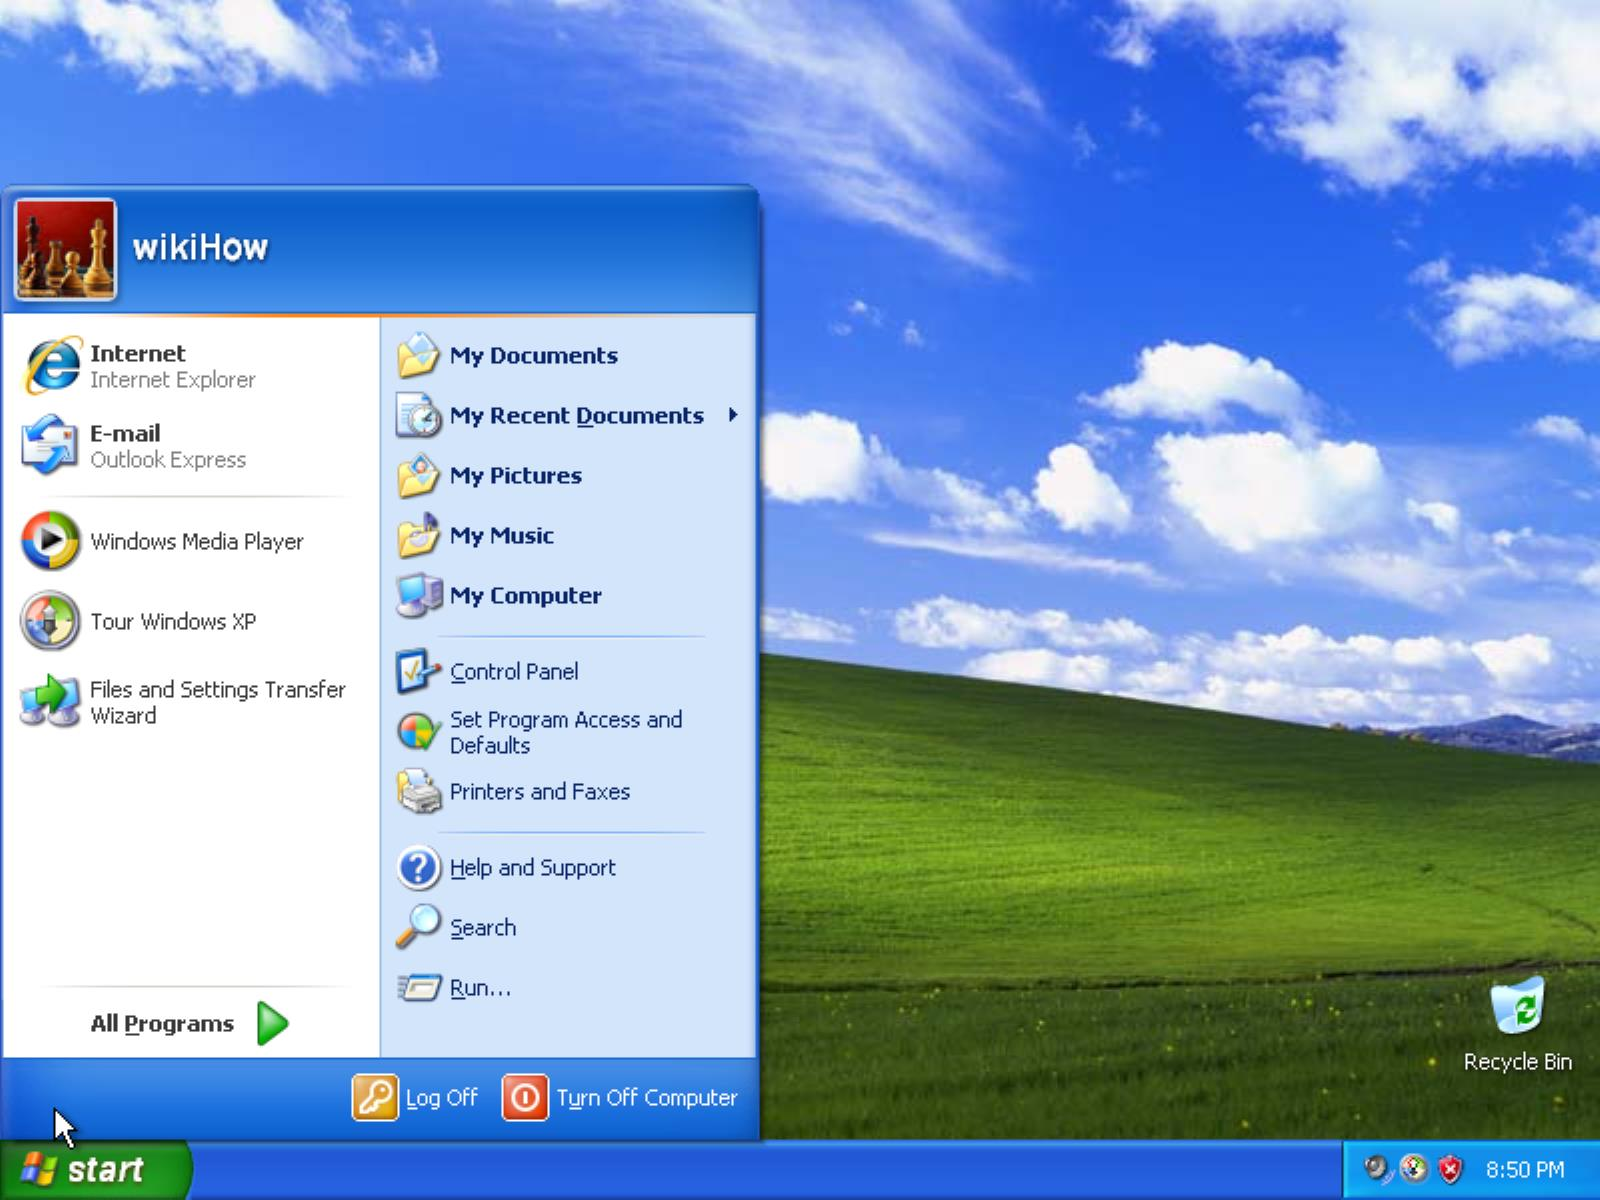
\includegraphics[width=1\textwidth]{figures/windowsxp.JPG}}
\caption{tampilan desktop di windows XP}
\label{windowsxp}
\end{figure}
% Windows Vista
	\section{Sejarah Windows Vista}
\ref{vista1}
		Windows Vista adalah sistem operasi berbasis dari Microsoft pada PC, Windows Vista dirilis pada tanggal 22 Juli 2005, Windows Vista ini lebih dikenal dengan Longhorn
	\subsection{Kelebihan dan Kekurangan Windows Vista}  \cite{russinovich2009windows}
		\subsubsection{Kelebihan:}
			1. Kualitas warna yang lebih tinggi, sehingga GUI (Grhapic User Interface) lebih bagus
			2. Bisa membaca RAM up to 16 GB
			3. Mendukung direct X 10
			4. Lebih cepat menjalankan program
			5. Banyak fitur baru yang tidak ada dalam versi sebelumnya
			6. Pencarian file lebih mudah 
		\subsubsection{Kekurangan:}
			1. Terdapat beberapa aplikasi yang belum support
			2. Terlalu banyak varian seri
	\subsection{Spesifikasi Hardware}
		\subsubsection{Minimum}
			Processor 800 Mhz(Pentium III atau Athlon)
			RAM 512 Mb
			Hard disk 40 Gb
			Graphic card bebas
		\subsubsection{Medium}
			Processor 2Ghz(Pentium 4 2,6 Ghz, Athlon XP 2800+ dll)
			RAM 1024 Mb
			Hard disk Sata 80 Gb
			Graphic card Direct x 9.0 (128 - 256 MB)
		\subsubsection{High}
			Processor 3 Ghz atau lebih, Processor Dual Core
			RAM 2048 Mb DDR II
			Hard disk Sata 120 Gb
			Graphic card Pixel Shader 2/3. (>256 MB)


\begin{figure}[ht]
\centerline{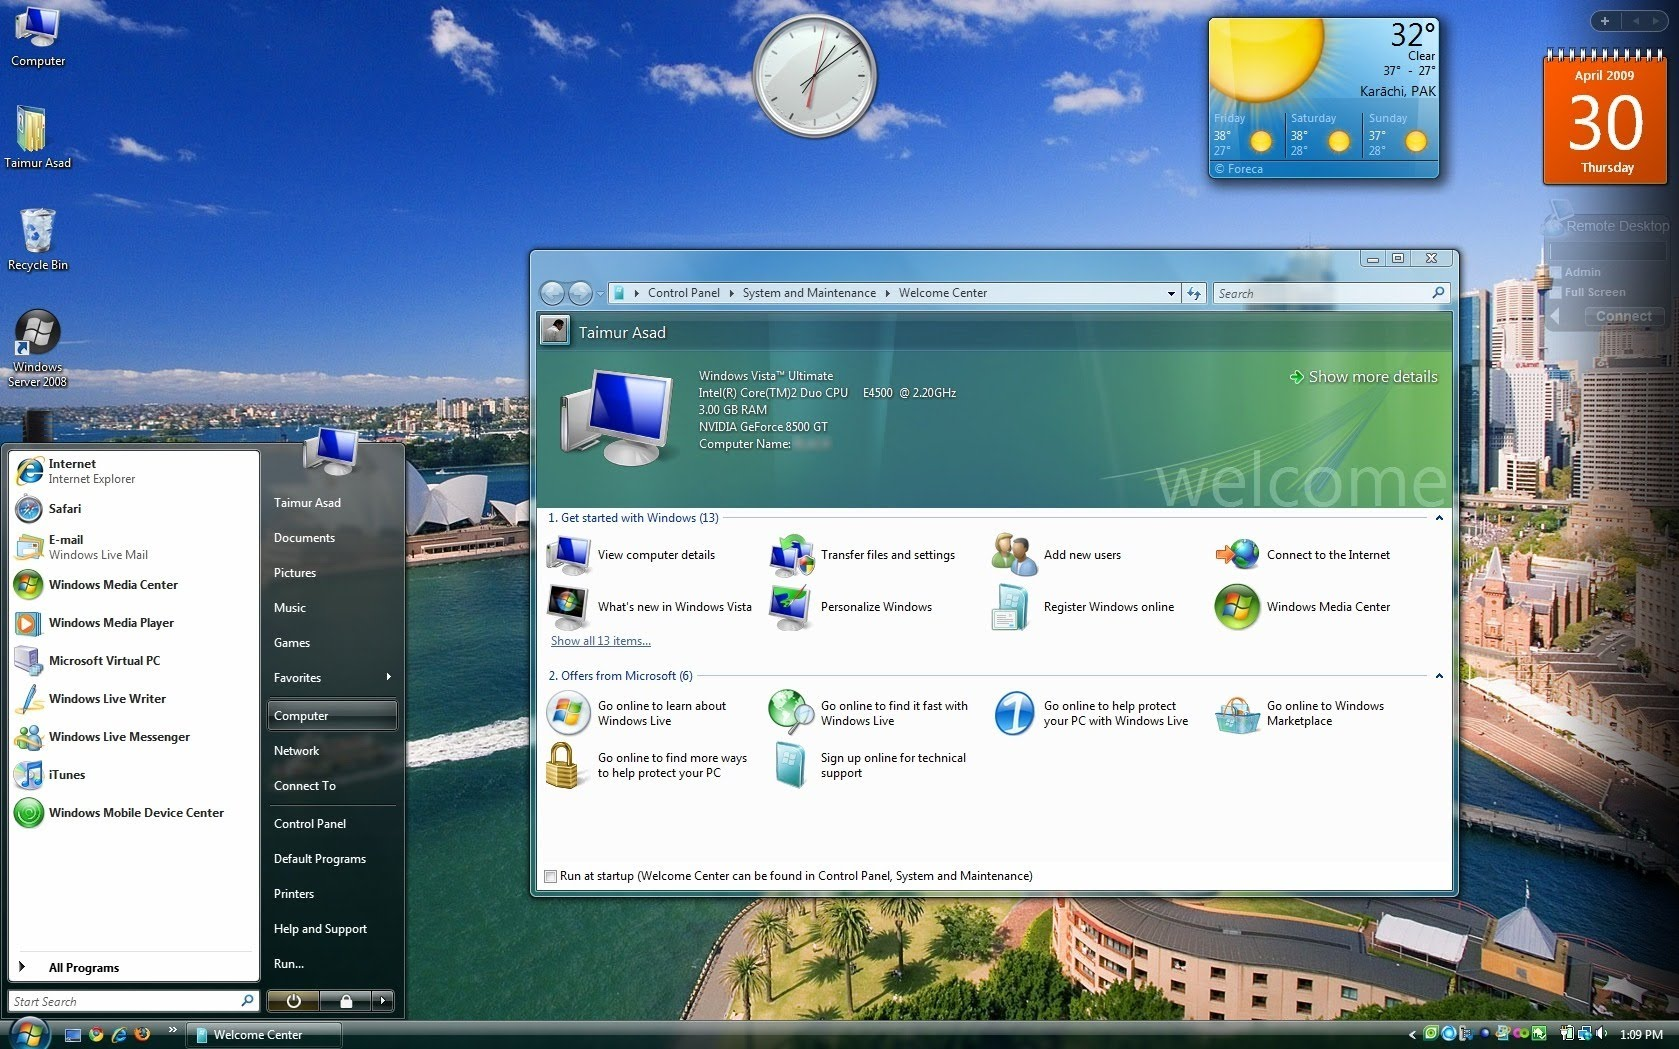
\includegraphics[width=1\textwidth]{figures/vista1.JPG}}
\caption{tampilan desktop di windows vista}
\label{vista1}
\end{figure}


% Windows 7
	\section{windows 7}
\ref{desktop7}
		Ada fitur fitur baru di windows 7 yang memberikan tantangan untuk memori
		dan juga menawarkan informasii yang dapat dipulihkan dan di ambil dari
		gambar,file,dan makalah. Fitur baru di windows 7 ini di kembangkan 
		metode analisis memori sesuai fitur masing masing. Metode ini
		berlandasan pada struktur data windows yangbernama dengan kernel
		processor. Proses yang berjalan pada windows ini ada 2 yaitu windows 7 
		7 dan 64-bit dan 32-bit windows 7
		\subsection{pendahuluan}
			Memori komputer sangat lah berguna sebagai sumber daya juga menawarkan
			Semua sistem operasi sepenuhnya dijalankan COROM, dan hampir semua
			semua informasi berhaga ada di memori komputer.
		\subsection{windows 7 edisi}
			1.windows 7 starter.
			2.windows 7 prefessional.
			3.windows 7 home basic.
			4.windows 7 enterprise.
			5.windows 7 ultimate.
			6.windows 7 home premium.
		\subsection{analisi windows 7 dan memori}
			\subsubsection{Gambaran dari windows 7}
				Ada pun perbadingan dengan widows 2000 dan windows xp, fitur windows 7 
				dijelaskan sebangai berikut. Strktur KPCR terletak di virtual OxFFDFFOOO
				di windows 7 KPCR dan KPCRB berada tidak terletak di alamat ini karna
				alamat struktur KPCR tidak dapat di temukan oleh lokasi stirng biner 
				00fdfff0fldff dalam gambar memo.(2) masing-masing objek karel adalah 
				prefxed oleh struktur objek header di windows 2000, dalam object header
				struktur windows 7, type variabel adalah bukan dengan variabel 
				Typelndex.(3)log peristiwa jendela telah berubah di windows 7. Fornat 
				yang bary untuk event log dan perpanjangan baru adalah \“EVTX\” 
				dan terletak di \“C: \Windows\System32\winevvt\Logs\”
		\subsubsection{alamat terjemahan}
			Karena alamat di memori umumnya di simpan sebagai alamat virtual,dan 
			alamat fisik digunakan untuk analasisi memori maka pentung untuk 
			menerjemahkan alamat virtual tersebut ke alamat fisik dengan 
			mempelajari terjemahan alamat prosesor intel. Proses terjemahan :  
			(1) Akuisisi struktur KPCR, variabel CurrentPrcb berikut nya ke 
			variable Self. Nilai variable diri diteruskan ke variavle currentPrcb 
			subsection(Registri)
			Registri windows adalah terdiri dari sejumlah fles biner yang berbeda 
			disebut juga dengan gatal-gatal pada disk. Sarang fles adalah unit 
			alokasi yang disebut blok. Blok utama dari sarang adalah blok dasar.

\cite{zhang2010exploratory} 

\begin{figure}[ht]
\centerline{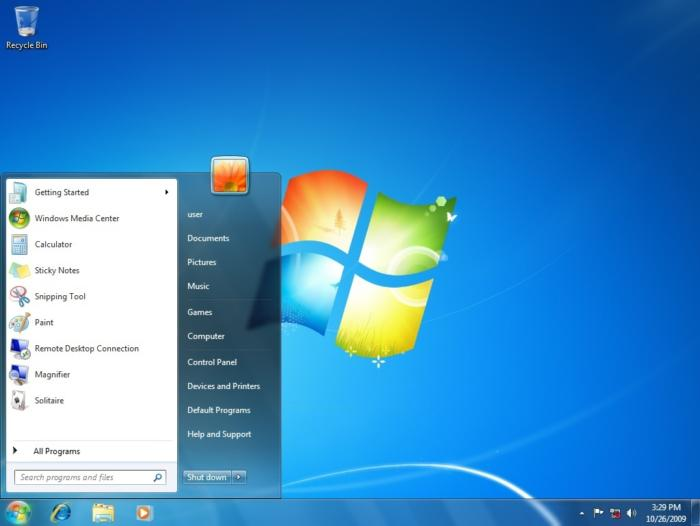
\includegraphics[width=1\textwidth]{figures/desktop7.JPG}}
\caption{tampilan desktop di windows 7}
\label{desktop7}
\end{figure}

% Windows server 2008
	\section{Windows Server 2008}
\ref{windowsserver2008}
	Windows Server 2008 merupakan sebuah sistem operasi yang powerful untuk PC server dan jaringan komputer. Windows Server 2008 diterbitkan sekitar 9 tahun yang lalu, tepatnya bulan februari tahun 2008.\cite{wahyono2009practice}
	\subsection{Sejarah dan Perkembangan}
		Sistem operasi Windows NT masih ada kaitannya dengan perkembangan Windows Server. Tahun 2007 Windows Server yang dikenal dengan nama \" Windows Server Codenamed Longhorn\" dikembangkan oleh microsoft. Longhorn diciptakan untuk menggantikan Windows Server 2003. Sesuai dengan keputusan Bill Gates tanggal 15 mei 2007 Windows Server Longhorn berubah menjadi Windows Server 2008.
	\subsection{Spesifikasi Sistem}
		\subsubsection{Prosesor}
		Minimal 1 GHz (X86 Processor) atau 1.4 GHz (x64 Processor)
		\subsubsection{Memori}
		Minimal yang dibutuhkan adalah 512 MB RAM. Maksimum untuk 32-Bit adalah 4 GB(standar) atau 64 GB(Enterpise dan Datacenter). Untuk yang 64-Bit Maksimumnya adalah 8 GB (Foundation), 32 GB (Standar), dan 2 TB (Enterpise, Datacenter, dan Itanium)
		\subsubsection{Hardisk}
		Minimum untuk 32-Bit adalah 20 GB dan untuk 64-Bit adalah 32 GB.
		\subsubsection{Display}
		Minimal Super VGA (800 x 600). Tetapi untuk pengalaman yang lebih baik menggunakan resolusi yang lebih tinggi.
	\subsection{Fitur penting}
	Windows Server 2008 mempunyai arsitektur dan fungsional lebih maju dibandingkan para pendahulunya. Dan juga memiliki kelibihin instalasi yang lebih mudah, diagnosis kesalahan, dan keamanan yang tangguh.

\begin{figure}[ht]
\centerline{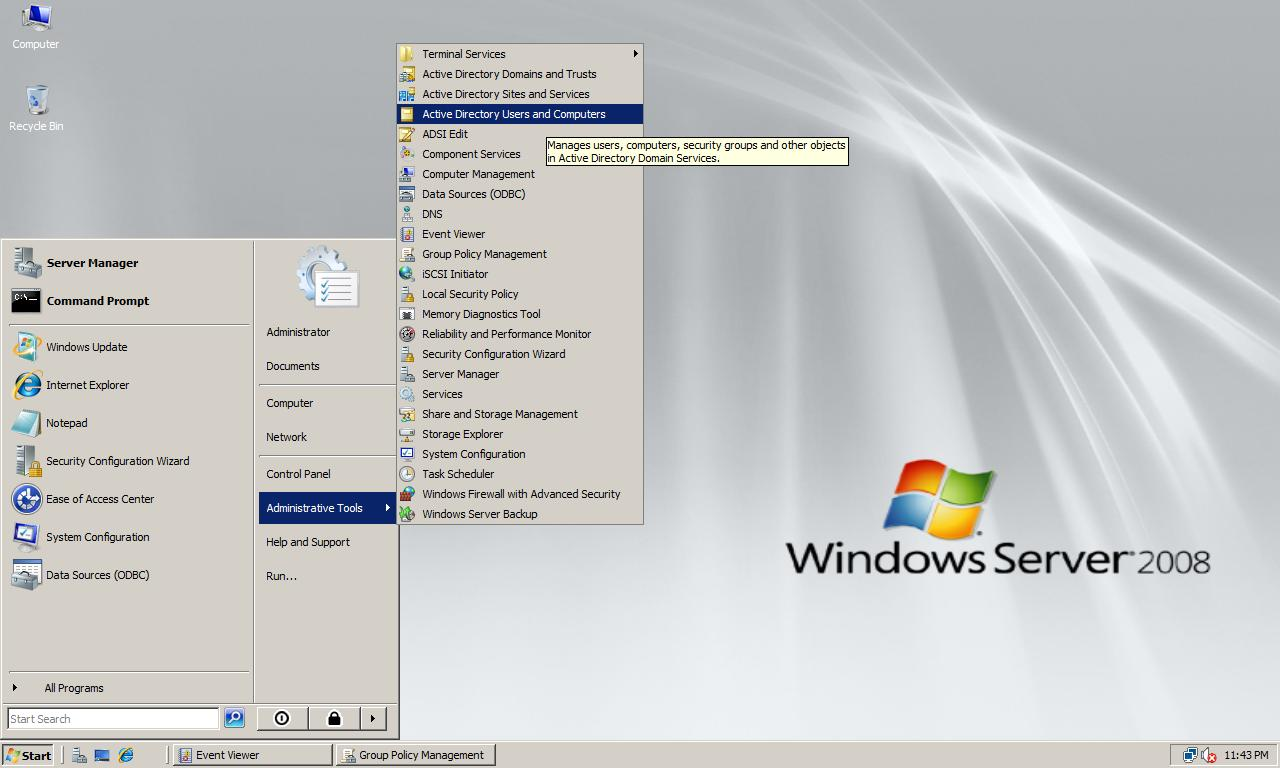
\includegraphics[width=1\textwidth]{figures/windowsserver2008.JPG}}
\caption{tampilan desktop di windows server 2008}
\label{windowsserver2008}
\end{figure}
% Windows 8
	\section{windows 8}
		\ref{tampilanwindows8} windows 8 diluncurkan oleh microsoft pada tahun 2012. dengan dirilisnya windows 8 ini mengubah format file hibernasi, memecah semua alat analisis yang ada.
		Dalam artikel yang ditulis oleh sylve mengemukakan bahwa pada saat itu matthieu suiche mempelajari format file hibernasi windows modern, pada bulan mei 2016 suiche mengumumkan versi beta Hibr2Bin yang mendukung file hibernasi windows 8. Hibr2Bin adalah alat yang mengubah file hibernasi windows menjadi gambar memori mentah sehingga bisa dianalisis dengan alat analisis memori yang secara native tidak mendukung penguraidan file hibernasi. Hibr2Bin diperbarui dan rilis secara terbuka pada akhir september 2016. \cite{sylve2017modern}
		\subsection{Fitur tambahan pada windows 8}
			Seperti yang di kutip pada artikel wahyu asri, windows 8 memiliki fitur tambahan yang memiliki kelebihan sebagai berikut :
			1. Optimalisasi untuk layar sentuh
			2. mendukung chip ARM
			3. toko aplikasi windows store
			4. mendukung NFC (Near Field Communication)
			5. waktu boot yang singkat
			6. Internet Explore 10
			7. Security lebih baik
			8. windows 8 tidak membutuhkan upgrade PC \cite{wahyu8review}

\begin{figure}[ht]
\centerline{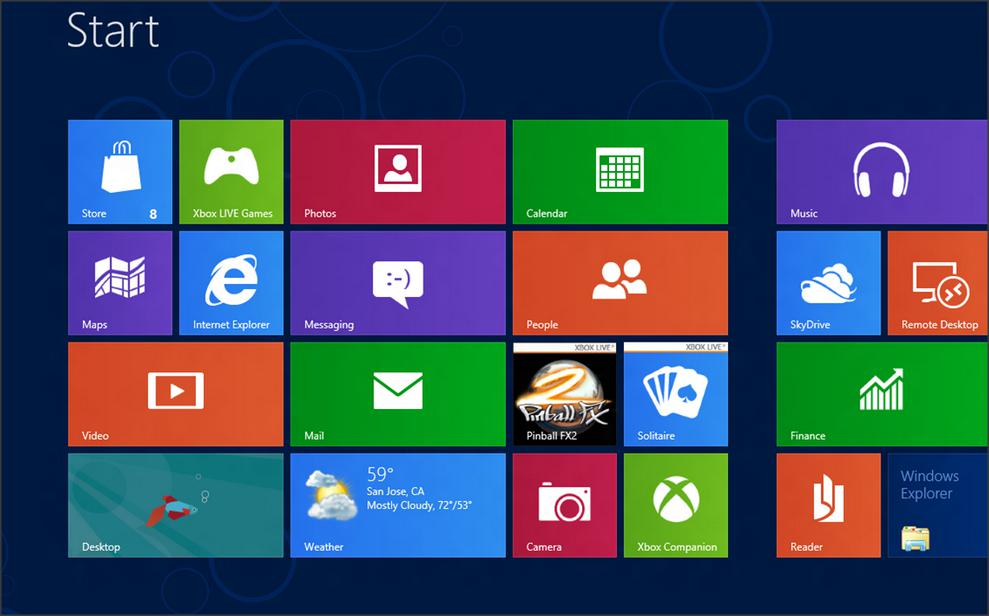
\includegraphics[width=1\textwidth]{figures/tampilanwindows8.JPG}}
\caption{tampilan desktop di windows 8.}
\label{tampilanwindows8}
\end{figure}


% Windows 2012 server
	\section{windows 2012 server}
		\ref{windows12} windows 2012 server merupakan sistem operasi penyempuraan dari windows sebelumnya yaitu windows 2008 R2. Windows 2012 ini merupakan versi server windows 8, pada windows 2012 ini, 
		menawarkan berbagai fitur-fitur baru dan juga peningkatan-peningkatan pada windows server. Windows ini resmi diperkenalkan pada november 2012. Tidak seperti windows 2008 R2 windows 
		2012 server ini tidak memiliki dukungan komputer yang berbasis itanium dan pada windows 2012 server ini banyak menekankan penggunaan cloud pribadi, sehingga pengguna dapat 
		mengaplikasikan dengan mudah. pada windows 2012 ini juga membantu memudahkan pengguna untuk menginstal mesin virtualnya secara efisien. disamping itu windows 2012 ini memiliki beberapa
		fitur untuk memperbaiki windows 2008 R2. dengan adanya semua fitur yang ada pada windows 2012 tersebut pengguna akan dapat mempelajari segala sesuatu mulai dari instalisasi, 
		keamanan, konfigurasi otomasi, pemantauan dan lain sebagainya yang dimuat dalam format resep praktis\cite{carvalho2012windows}
		\subsection{edisi windows server 2012}
			1.windows server 2012 foundation
			2.windows server 2012 essantiasis
			3.windows server 2012 standard
			4.windows server 2012 datacenter
			5.windows multipoint server 2012

\begin{figure}[ht]
\centerline{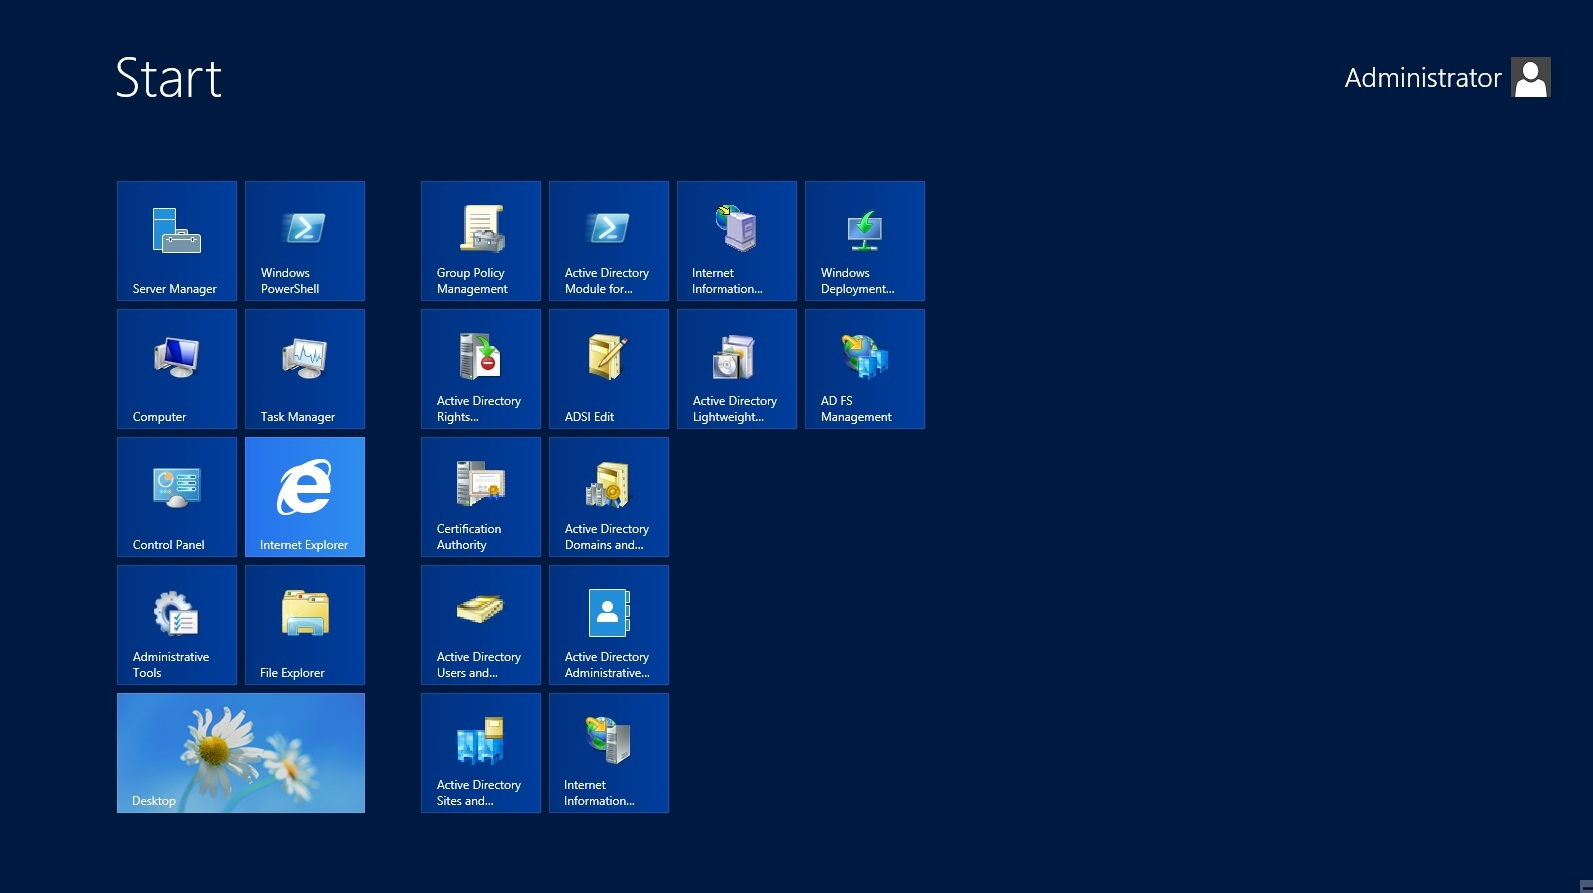
\includegraphics[width=1\textwidth]{figures/windows12.JPG}}
\caption{tampilan desktop di windows server 2012}
\label{windows12}
\end{figure}

	
% Windows 10
	\section{windows10}
		Windows 10 merupakan salah satu sistem operasi yang dirilis oleh perusahaan multinasional Microsoft Corporation pada tanggal 29 juli 2015. windows 10 dikenal sebagai suatu sistem 
		operasi yang selalu menerima pembaharuan terhadap fitur fitur yaang ada didalamnya. Pada awal peluncurannya, Microsoft Corporation mengadakan sebuah kampanye periklanan yang 
		mengenai perilisan windows 10 yang memiliki tema \"Upgrade Your World\". Dalam iklan tersebut, perusahaan ini menggunakan tagline \"Cara Yang Lebih Manusiawi Untuk Diakses\" berikut gambar dari windows 10 \ref{tampilanwindows10}
		\subsection{keunggulan dan fitur fitur windows 10}
			Dalam sebuah buku yang ditulis oleh JJ. Foster menyebutkan sistem operasi versi terbaru dari Microsoft ini mampu membangun keselarasan pengalaman dan fungsionalitas pengguna 
			dalam perbedaan kelas perangkat \cite{foster2001data} 
			Pada fitur windows 10 terdapat Windows Store yang berfungsi sebagai wadah untuk mendownload aplikasi. gambar ditampilkan sebagai berikut\ref{Store}, Groove Music sebagai 
			aplikasi pemutar musik. gambar ditampilkan sebagai berikut\ref{Groove}, dan Films dan Tv sebagai aplikasi pemutar video dan film. Gambar ditampilkan sebagai berikut\ref{Films_Tv}. 
			Tidak hanya itu, Windows 10 juga menyedikan fitur Xbox yang memungkinkan para pengguna untuk menjelajah perpustakaan permainan. Gambar ditampilkan sebagai berikut\ref{Xbox}
		\subsection{fitur yang dihapus}
			Akan tetapi, ada juga fitur yang tidak dilanjutkan pengembangan bahkan dihapus saat diupgrade dari versi sebelumnyl.a. Fitur tersebut adalah:
			-Windows Media Center
			-Aplikasi makanan dan minuman
			-Aplikasi kesehatan
			-dan aplikasi travel/perjalanan.


\begin{figure}[ht]
\centerline{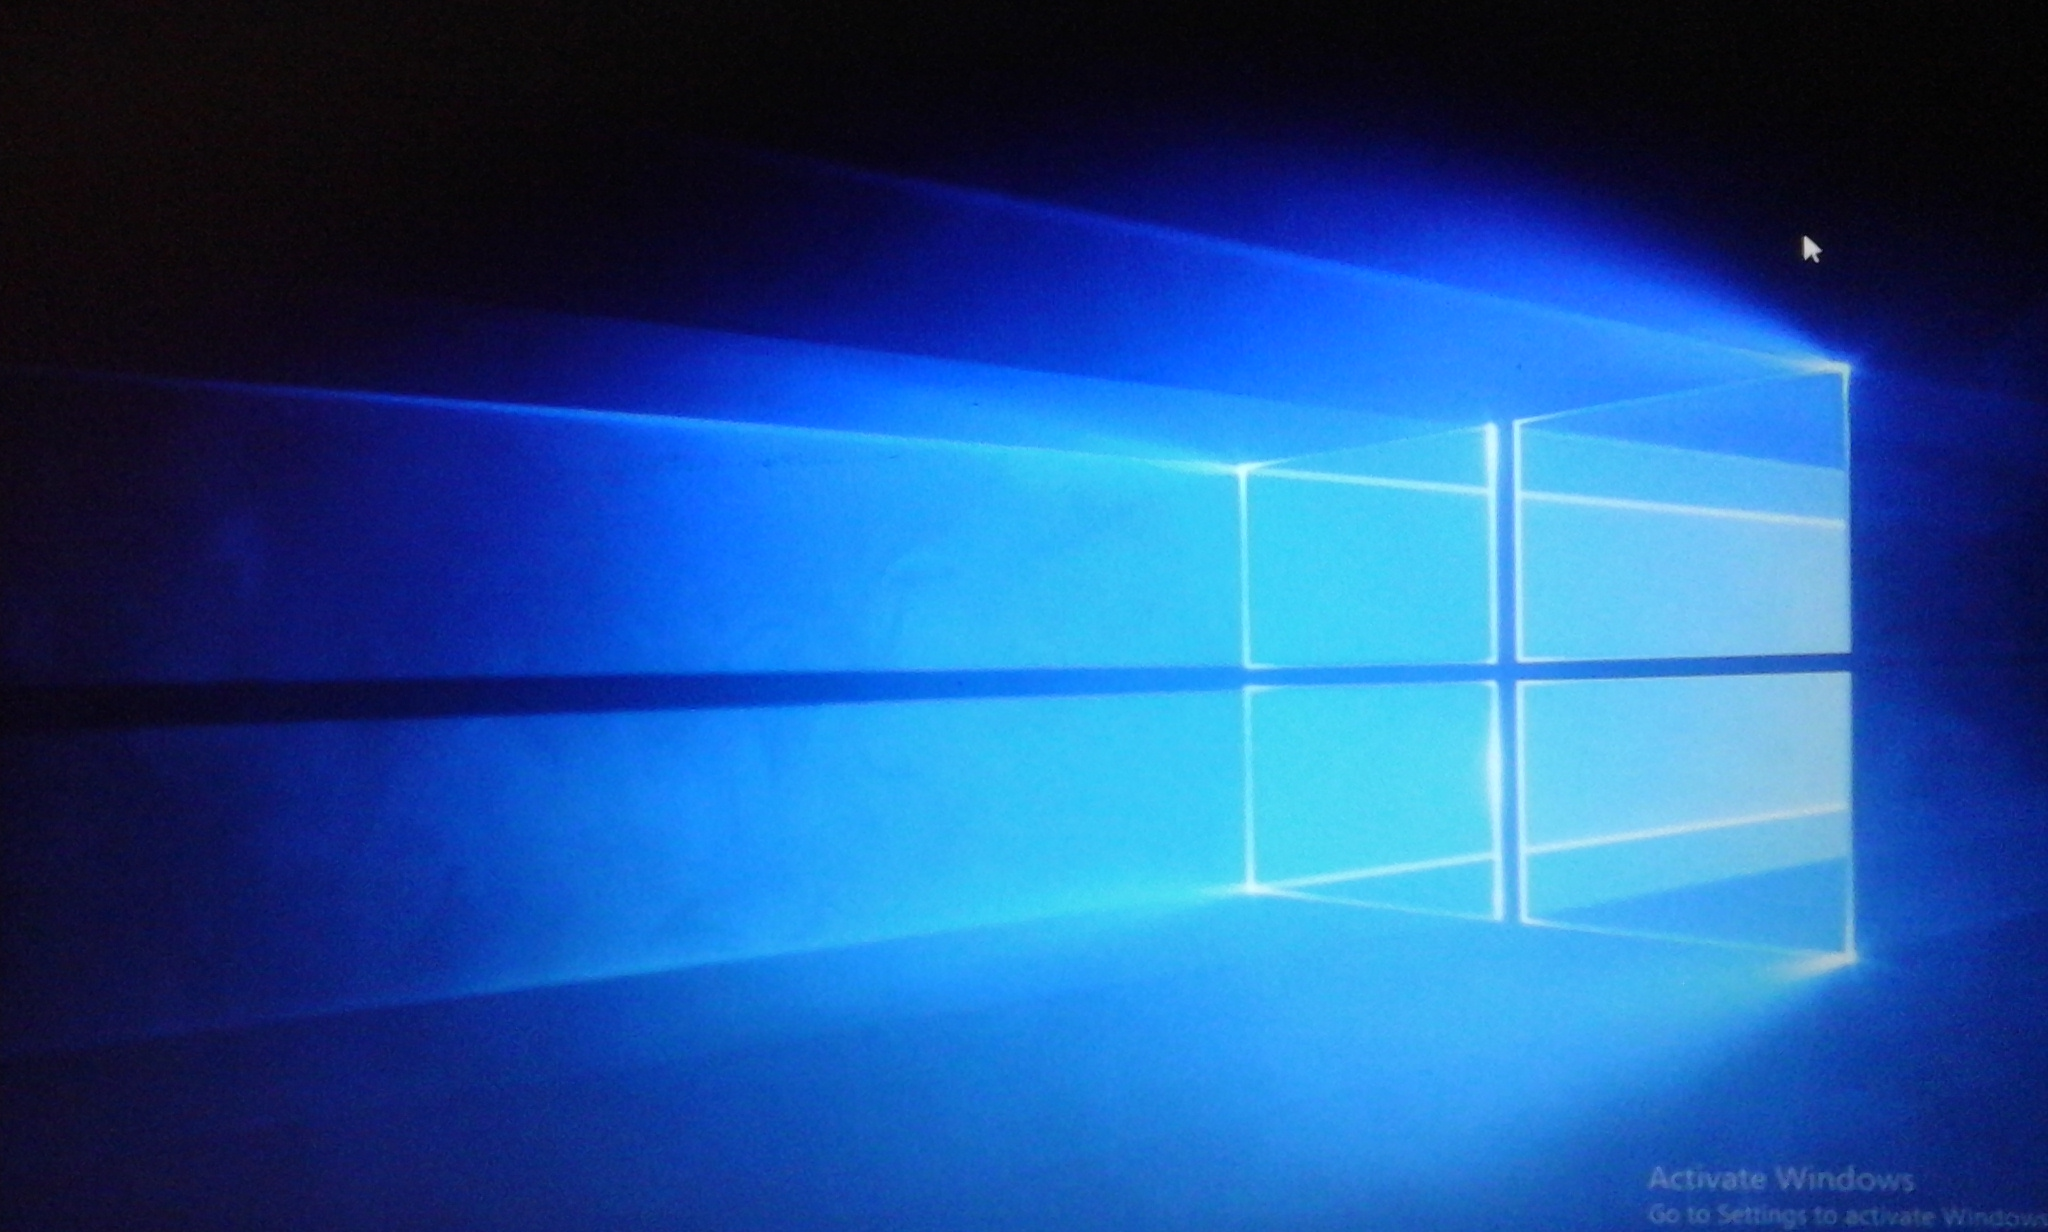
\includegraphics[width=1\textwidth]{figures/tampilanwindows10.JPG}}
\caption{tampilan desktop di windows 10.}
\label{tampilanwindows10}
\end{figure}

\chapter[Linux]
{Software\\ linux}
% Nama Kelompok : Linux
% Kelas : D4 TI 1A
% 1. Kadek Diva Krishna Murti (1174006)
% 2. Duvan Silalahi (1174011)
% 3. Oniwaldus (1174005)
% 4. Choirul Anam (1174004)
% 5. Sri Rahayu (1174015)
% 6. Ilham Habibi (1174028)



\begin{figure}[ht]
\centerline{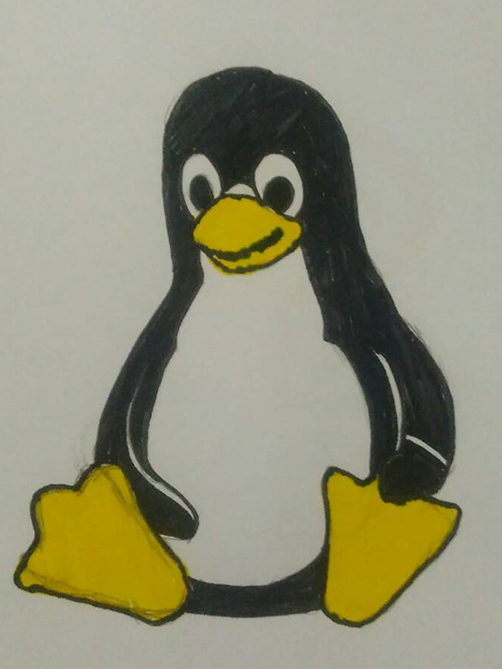
\includegraphics[width=0.5\textwidth]{figures/linux.jpg}}
\caption{Logo Linux.}
\label{Linux}
\end{figure}

Menurut Wahana Komputer dalam bukunya yang berjudul Mari Mengenal Linux menyebutkan bahwa Linux merupakan sebuah sistem operasi yang mirip dengan UNIX, dan merupakan implementasi independen dari sistem operasi POSIX, dengan ekstensi SYSV dan BSD sistem operasi UNIX, yang berjalan di mesin keluarga Intel 80386DX, atau yang lebih baru. Pada perkembangan berikutnya, Linux dapat berjalan di beberapa mesin lainnya seperti Sun Sparc, Mac, PowerPC, DEC Alpha, dan PPC mk86.\cite{komputer2005mari}

Linux adalah sistem operasi yang diedarkan secara gratis di bawah lisensi GNU General Public License (GPL), yang berarti source code Linux tersedia. Dengan begitu program tersebut dapat diubah, diadaptasi, maupun dikembangkan lebih lanjut oleh siapapun.

\section{Sejarah} 

Menurut Wahana Komputer dalam bukunya yang berjudul Mari Mengenal Linux menyebutkan bahwa dahulu Linux adalah proyek hobi yang dikerjakan oleh seorang mahasiswa Finlandia yang bernama Linus Torvalds. Dalam mengerjakan proyek hobinya tersebut, Linus Torvalds memperoleh inspirasi dari Minix, yaitu suatu sistem UNIX kecil yang dikembangkan oleh Andy Tanenbaum. Linux versi 0.01 dikerjakan sekitar bulan Agustus 1991. Kemudian pada tanggal 5 Oktober 1991 Linus Torvalds mengumumkan versi resmi dari Linux, yaitu 0.02. Versi ini hanya dapat menjalankan Bash (GNU Bourne Again Shell) dan gcc (GNU C Compiler). Meskipun Linux bukan merupakan sistem Unix resmi, namun Linux memiliki dasar warisan, budaya, arsitektur dan pengalaman sistem operasi Unix, sebuah sistem operasi yang sudah berjalan selama 28 tahun lebih. \cite{komputer2005mari}

\subsection{Pengenalan}

Menurut artikel Dasar-Dasar Linux menyebutkan bahwa Linus Torvalds membuat Kernel Linux, yaitu sebuah core Linux, di atas Minix dengan menggunakan bahasa C. Linux memiliki lisensi GNU, sebuah lisensi yang dikeluarkan untuk memungkinkan seseorang mendistribusikan, mengembangkan, dan memodifikasi source code suatu program secara gratis dan bebas. Pembuatan Linux di lakukan secara gotong royong oleh banyak programmer yang kebanyakan C/C++ Programmer di seluruh dunia via internet. Logo Linux adalah seekor penguin seperti gambar\ref{Linux}. Karena pada saat pengembangan Linux, Torvalds pernah di patuk oleh Penguin di sebuah kebun binatang yang menyebabkan dirinya demam dan dia bercita-cita agar orang lain dapat \"demam\" Linux. Nama Linux sendiri di adaptasi dari nama nya Linus. Saat ini, Linux memiliki beberapa Desktop Environment yang berbasis Grafis yaitu, KDE (K Desktop Environment) dan GNOME (GNU Network Object Model Environment). \cite{sofwan2003dasar}

\subsection{Aplikasi Yang Terdapat di Linux}

Menurut Wahana Komputer dalam bukunya yang berjudul Mari Mengenal Linux menyebutkan bahwa karena kernel Linux dikembangkan dengan usaha yang independent, banyak aplikasi yang tersedia, sebagai contoh, C Compiler menggunakan gcc dari Free Software Foundation GNU’s Project. Compiler ini banyak dipergunakan  pada lingkungan Hewlett-Packard dan Sun. Sekarang, banyak aplikasi Linux yang dapat dipergunakan untuk keperluan perkantoran seperti untuk spreadsheet, word processor, database dan Star Office yang merupakan program editor grafis yang memiliki tampilan dan fungsi layaknya Microsoft Office. Selain itu di Linux juga sudah tersedia versi Corel dan aplikasi seperti Matlab yang pada Linux dikenal sebagai Scilab. \cite{komputer2005mari}

Sekarang Linux merupakan sistem UNIX yang bisa digunakan untuk jaringan (networking), pengembangan software, bahkan untuk kebutuhan sehari-hari. Linux merupakan alternatif sistem operasi yang bisa didapatkan secara gratis jika dibandingkan dengan sistem operasi komersial lainnya dan dengan kemampuan yang setara atau bahkan lebih.


\section{Distribusi Linux}

Berikut ini beberapa distribusi (distro) Linux yang banyak peminatnya di Indonesia.

\begin{enumerate}

\item \textbf{Debian Linux}

\begin{figure}[ht]
\centerline{
\includegraphics[width=0.4\textwidth]{figures/debian.jpg}}
\caption{Logo Debian Linux.}
\label{Debian}
\end{figure}

Menurut Wahana Komputer dalam bukunya yang berjudul Mari Mengenal Linux menyebutkan bahwa Debian merupakan distribusi dari Linux yang kurang terkenal, namun banyak penggunanya dari kalangan teknis. Mereka puas karena kestabilannya. Selain itu, format paket programnya yang menggunakan DEB dianggap lebih stabil daripada RPM menurut kalangan teknis.
Versi terakhir dari Debian adalah versi 2.1, yang dirilis pada tahun 1999. Dibandingkan dengan distribusi lainnya, Debian termasuk yang jarang dalam meng-update programnya. Debian juga sudah menggunakan metode autodetect untuk penggunaan peripheral pada komputer. \cite{komputer2005mari} Debian Linux memiliki logo seperti gambar \ref{Debian}.

Jika Anda ingin tahu lebih lanjut mengenai Debian Linux ataupun men-download programnya secara langsung, Anda bisa mengunjungi situsnya di http://www.debian.org

\textbf{\item RedHat Linux}


\begin{figure}[ht]
\centerline{
\includegraphics[width=0.4\textwidth]{figures/redhat.jpg}}
\caption{Logo RedHat Linux.}
\label{RedHat}
\end{figure}

Menurut Wahana Komputer dalam bukunya yang berjudul Mari Mengenal Linux menyebutkan bahwa  Redhat merupakan distribusi Linux yang paling popular di Indonesia dan Amerika yang dirancang khusus untuk server. RedHat di akui sebagai server tercepat dibandingkan dengan distribusi Linux lainnya untuk server. Selain dapat diguanakan sebagai server tercepat, RedHat juga dapat dipakai sebagai klien maupun digunakan sebagai desktop rumah tangga alias PC standlone. Saat ini Redhat sudah beredar dengan versi 6.2, menggunakan Standard Desktop Gnome.

Kelebihan lain dari RedHat adalah kemudahan dalam hal instalasinya. Ini merupakan revolusioner Linux. Ketika distribusi linux lainnya membuat penggunanya awalnya menjadi putus asa pada saat prosedur instalasinya, RedHat hadir dengan prosedur instalasi yang termudah pada masanya.
Hal revolusioner lainnya adalah RedHat membuat format paket program RPM menjadi standar baku file biner pada Linux, yang kemudian digunakan oleh distribusi lainnya seperti SuSE, Mandrake dan Caldera. \cite{komputer2005mari} Redhat Linux memiliki logo seperti gambar \ref{RedHat}.

Jika Anda ingin tahu lebih lanjut mengenai RedHat Linux ataupun men-download programnya secara langsung, Anda bisa mengunjungi situsnya di http://www.redhat.com

\textbf{\item Mandrake Linux}


\begin{figure}[ht]
\centerline{
\includegraphics[width=0.4\textwidth]{figures/mandrake.jpg}}
\caption{Logo Mandrake Linux.}
\label{Mandrake}
\end{figure}

Menurut Wahana Komputer dalam bukunya yang berjudul Mari Mengenal Linux menyebutkan bahwa Mandrake adalah saudara muda dari RedHat, karena keduanya dibuat oleh satu distribusi. Bila RedHat direkomendikasikan sebagai server, maka Mandrake direkomendasikan oleh pembuat distro RedHat sebagai klien yang handal, namun diutamakan yang menggunakan prosesor Pentium. Meskipun demikian, tidak menutup kemungkinan penggunaan Mandrake sebagai server yang handal juga.

Tujuan diciptakannya Mandrake pada awalnya adalah untuk mempermudah penggunanya dalam melakukan instalasi dan penggunaan Linux. Sebelum diluncurkannya Corel Linux, Mandrake merupakan salah satu distribusi Linux yang paling populer. Jika RedHat keluar dengan desktop manager menggunakan Gnome, maka Mandrake keluar dengan desktop manager KDE buatan SuSE Jerman. Saat ini Mandrake sudah keluar dengan versi 7.1. \cite{komputer2005mari} Mandrake Linux memiliki logo seperti gambar \ref{Mandrake}.

Jika Anda ingin tahu lebih lanjut mengenai Mandrake Linux ataupun men-download programnya secara langsung, Anda bisa mengunjungi situsnya di http://www.linux-mandrake.com

\textbf{\item Caldera Open Linux}


\begin{figure}[ht]
\centerline{
\includegraphics[width=0.4\textwidth]{figures/caldera.jpg}}
\caption{Logo Caldera Open Linux.}
\label{Caldera}
\end{figure}

Menurut Wahana Komputer dalam bukunya yang berjudul Mari Mengenal Linux menyebutkan bahwa Caldera merupakan merupakan distribusi Linux yang dirancang untuk mempermudah pemakainya dalam pengoperasiannya. Caldera sendiri dirancang sebagai distribusi Linux yang keselurahannya dalam bentuk grafis. Sejak mulai instalasi hingga setting hardware, semuanya dalam bentuk grafis. Yang mengagumkan adalah pada saat melakukan instalasi Caldera, Anda akan disuguhi game tetris untuk mengisi waktu, sembari menunggu transfer program. Selain itu Caldera merupakan distribusi Linux pertama yang menggunakan auto-detect hardware (seperti plug dan  play pada Mac). \cite{komputer2005mari} Caldera Linux memiliki logo seperti gambar \ref{Caldera}.

Jika Anda ingin tahu lebih lanjut mengenai Caldera Open Linux ataupun men-download programnya secara langsung, Anda bisa mengunjungi situsnya di http://www.caldera-system.com

\textbf{\item Slackware Linux}


\begin{figure}[ht]
\centerline{
\includegraphics[width=0.4\textwidth]{figures/slackware.jpg}}
\caption{Logo Slackware Linux.}
\label{Slackware}
\end{figure}

Menurut Wahana Komputer dalam bukunya yang berjudul Mari Mengenal Linux menyebutkan bahwa Slackware dibuat oleh Patrick Volkerding, Slackware merupakan distribusi Linux yang pertama, dengan tampilan yang sederhana tapi penggunaannya manual tidak seperti produk Linux yang lain. Biasanya Slackware digunakan oleh pengguna Linux yang sudah pro atau bisa juga yang ingin menjadi pengguna Linux yang pro. Slackware awalnya turunan dari Softlanding Linux System dan merupakan yang paling populer dari distribusi Linux asli. Versi Slackware Linux yang pertama tersedia di publik adalah versi 1.0 yang rilis pada 16 juli 1993. Slackware Linux mengacu pada prinsip KISS (Keep It Simple Stupid). \cite{ komputer2005mari}. Slackware Linux memiliki logo seperti gambar \ref{Slackware}.

Jika Anda ingin tahu lebih lanjut mengenai Slackware Linux ataupun men-download programnya secara langsung, Anda bisa mengunjungi situsnya di http://www.slackware.com

\textbf{\item Suse Linux}


\begin{figure}[ht]
\centerline{
\includegraphics[width=0.4\textwidth]{figures/suse.jpg}}
\caption{Logo Suse Linux.}
\label{Suse}
\end{figure}

Menurut Wahana Komputer dalam bukunya yang berjudul Mari Mengenal Linux menyebutkan bahwa Suse Linux merupakan distribusi Linux yang sistemnya dioperasikan di atas kernel. Suse Linux merupakan produk Linux yang sangat populer di Negara Eropa. Dilengkapi dengan KDE dan central setting YaST (Yet Another Settup Tools) yang digunakan sebagai sistem operasi untuk deskop dan server. Suse bermula pada tahun 1990-an yang didirikan oleh perusahaan Novell yang dimana Linux terdiri dari 50 keping disket dan dapat di unduh atau diambil lewat internet. Ada 2 macam jenis Suse Linux yaitu, Suse Linux Enterprise dan Open Suse. Suse Linux Enterprise terdiri dari 2 paket yaitu, Suse Linux Enterprise Server dan Suse Linux Enterprise Deskop. Open Suse merupakan sebuah proyek masyarakat yang disponsori oleh Novell dan dirancang untuk pengguna rumah. \cite{komputer2005mari} Suse Linux memiliki logo seperti gambar \ref{Suse}.

Jika Anda ingin tahu lebih lanjut mengenai Suse Linux ataupun men-download programnya secara langsung, Anda bisa mengunjungi situsnya di http://www.suse.com

\textbf{\item Corel Linux}


\begin{figure}[ht]
\centerline{
\includegraphics[width=0.4\textwidth]{figures/corel.jpg}}
\caption{Logo Corel Linux.}
\label{Corel}
\end{figure}

Menurut Wahana Komputer dalam bukunya yang berjudul Mari Mengenal Linux menyebutkan bahwa Corel Linux dibuat oleh distribusi Linux yaitu Debian. Corel Linux mendukung operasi sistem open source dibawah naungan GNU. Harganya juga sangat terjangkau dan dapat langsung di instal dengan sistem operasi lain dan juga bisa tanpa sistem operasi lain. Corel Linux juga bisa dinstal pada partisi dan file sistem Windows yang menjadikan corel linux seolah-olah adalah program aplikasi Windows. Corel Linux dirancang sebagai End-User. Pada Corel Linux semuanya serba grafis, dimulai saat instalasi sampai pada boot sistem. Pada Corel Linux kita tidak akan menjumpai baris teks seperti pada Linux yang lain, atau bahkan seperti pada Windows yang masih kelihatan baris teks. Semua sistem Corel Linux ini sangat sederhana sampai pada setting jaringannya lebih sederhana daripada Windows. \cite{komputer2005mari} Corel Linux memiliki logo seperti gambar \ref{Corel}.

Jika Anda ingin tahu lebih lanjut mengenai Corel Linux ataupun men-download programnya secara langsung, Anda bisa mengunjungi situsnya di http://www.linux.corel.com

\textbf{ \item Turbo Linux}


\begin{figure}[ht]
\centerline{
\includegraphics[width=0.4\textwidth]{figures/turbo.jpg}}
\caption{Logo Turbo Linux.}
\label{Turbo}
\end{figure}

Menurut Wahana Komputer dalam bukunya yang berjudul Mari Mengenal Linux menyebutkan bahwa Turbo Linux sangat populer dan terkenal di Asia. Turbo Linux menduduki posisi pertama pada Linux pilihan. Turbo Linux diciptakan dari berbagai program-program under Linux atau UNIX. Turbo Linux mendesain produknya dengan menggabungkan beberapa kelebihan dari open source dan dari perangkat lunak komersial. Turbo Linux menyertakan Cross Platform Management Software dalam produk-produk work station server dan clustering yang memungkinkan kemudahan dalam memanage networks dan sistem. Ada beberapa fitur Turbo Linux yaitu, Kernel 2.4.5, Glibc 2.2.3, Gcc 2.95.3, Xfree86 4.1.10, Rpm 4.0.2, Kde 2.1.2, Gnome 1.4. \cite{komputer2005mari} Turbo Linux memiliki logo seperti gambar \ref{Turbo}.

Jika Anda ingin tahu lebih lanjut mengenai Turbo Linux ataupun men-download programnya secara langsung, Anda bisa mengunjungi situsnya di http://www.turbo-linux.com



\end{enumerate}

\section{Kelebihan Linux}

Berikut ini beberapa kelebihan dari penggunaan Sistem Operasi Linux, di antaranya adalah:

\begin{itemize}

\item Merupakan salah satu sistem operasi yang bersifat open source, yang berarti penggunanya dapat melihat maupun mengubah source codenya tanpa terkena sanksi.

\item Merupakan salah satu sistem operasi yang freeware di bawah lisensi GNU, yang berarti penggunanya tidak harus mengeluarkan biaya untuk memiliki sistem operasi ini.

\item Tidak memerlukan spesifikasi hardware yang tinggi untuk menjalankan sistem operasi ini.

\item Linux kebal  terhadap virus karena Linux mendukung adanya file permissions (ijin file), yang dapat mencegah perubahan atau penghapusan file tanpa ijin dari pemiliknya.

\item Lebih dari satu orang dapat menggunakan program yang sama atau berbeda dari satu mesin yang sama, pada saat bersamaan, di terminal yang sama atau berbeda.

\item Dalam satu komputer, pengguna dapat melakukan login dengan nama user yang sama atau berbeda lebih dari satu kali, tanpa perlu menutup sesi sebelumnya.

\item Mengeksekusi suatu program dan mengakses data dapat dilakukan secara bersama-sama tanpa harus khawatir terjadi hang atau stack.

\item Dalam penggunaannya Linux sangat stabil sehingga bisa mengcopy, mengedit, menghapus satu file atau data secara bersamaan pada saat data atau file tersebut dieksekusi.

\item Jumlah login user atau operator yang dimiliki tidak terbatas sehingga user bisa mencapai 254 klien secara bersamaan dan dilengkapi dengan password.

\item Linux dapat digunakan sebagai Web Server atau sebagai FTP Server.

\item Linux mendukung fasilitas GUI (Graphic User Interface).

\end{itemize}

\section{Kelemahan Linux}

Berikut ini beberapa kelemahan dari penggunaan Sistem Operasi Linux, di antaranya adalah:

\begin{itemize}

\item Cara penggunaanya sangat berbeda sekali dengan sistem operasi lainnya seperti Windows sehingga perlu waktu dan tenaga ekstra untuk mempelajari penggunaanya. Apalagi bagi yang baru belajar komputer akan mengalami kesulitan dalam penggunaannya.

\item Banyak aplikasi-aplikasi yang belum mendukung penggunaanya dalam Linux.

\item Tidak dapat mendukung beberapa hardware-hardware tertentu.

\item Sedikit penggunanya, hal ini menyebabkan sedikit juga orang-orang yang dapat di jadikan ajang bertanya sesama pengguna Linux.

\end{itemize}


\chapter[Macintosh]
{Software\\ mac}
% Nama Kelompok : Macintosh
% Kelas : D4 TI 1A
% Anggota : 
% 1. Harun   	1174027
% 2. Fahmi   	1174021
% 3. Kukuh		1174016
% 4. Izzah		1174013
% 5. Rizal		1174014
% 6. Lawimner	1174030




Artikel tentang sejarah Mac OS dari masa ke masa

\section{penjelasan singkat}
Sebelum kita mengetahui lebih dalam lagi tentang MAC OS sebaiknya kita mengenal penciptanya terlebih dahulu
pada zaman dahulu kala hiduplah seorang anak yang bernama \"Steve Jobs\" yang lahir di kota San Fransisco California 
pada tanggal 24 Februari 1955. ia adalah seoarang yatim piatu yang di adopsi oleh Paul dan Clara Jobs.
Berikut perjalanan hidup dan karir Steve Jobs hingga embusan nafas terakhir : 

1955 : di tahun 1955 beliau lahir pada tanggal 24 Februari

1972 : beliau mmelanjutkan pendidikan di perkuliahan tepatnya di Reed College, Portland, Oregon. Tapi ia di drop out setelah semester pertama masuk kuliah

1974 : ia bekerja untuk pembuatan video game Atari dan mengikuti ia juga berkesempatan mengikuti pertemuan Homebrew Computer Club dengan Steve Wozniak, seorang teman sekolahnya yang lebih tua beberapa tahun dengannya. dan Ini merupakan sejenis seminar atau juga bisa di sebut dengan pertemuan yang membahas tema-tema komputer

1975 : Jobs dan Woz kembali menghadiri acara di Homebrew Computer Club Meetings. 

1976 : Komputer Apple tercipta pada April Mob yang jatuh pada tanggal 1 April, tak lama sejak itu jobs dan wozniak membuat sebuah komputer sirkuit baru di garasi Silicon Valley. Pendiri ketiga Apple, Ron Wayne, meninggalkan kerja sama ini, karena setelah hanya dua minggu bekerja. Komputer Apple I dijual pada musim panas seharga US\$ 666,66 atau sekitar Rp.8.658.000 per unit nya

1977 : Apple bergabung dengan beberapa pihak perusahaan untuk membuat kerja sama join venture. Dari situ terciptalah Apple II, komputer pribadi pertama dengan menggunakan grafis berwarna. Pendapatan perusahaan mencapai US\$ 1 juta.

1979 : selanjutnya Jobs mengunjungi Xerox Palo Alto Research Center (PARC). Dari sini ia mendapatkan sebuah ide untuk membuat sebuah komputer dengan graphical user interface yang sangat luas yaitu dapat memfasilitasi tampilan dengan pilihan pada layar berbentuk simbol-simbol 

1980 : Apple kembali mencatatkan sahamnya di bursa saham. Perusahaan mendapatkan dana sebesar US\$ 110 juta. Ini merupakan initial public offering (IPO) terbesar di tahun itu

1982 : adapun Pendapatan per tahun nya perusahaan Apple meningkat hingga mencapai US\$ 1 miliar

1983 : Komputer Apple II dengan menu ikon di layar atau mereka menamakan komputer ini The Lisa diluncurkan ke pasaran dan membuat kehebohan. beliau membujuk John Sculley untuk meninggalkan pekerjaannya di Pepsico Inc. untuk menjadi CEO di perusaan Apple

1984 : untuk meningkatkan daya jual Icon Macintosh di iklankan secara komersial selama acara Super Bowl.dan Macintosh mulai dijual ke pasar

1985 : Jobs dan Sculley terlibat masalah hingga membuat Jobs memutuskan untuk mundur dari perusahaan. seiring masalah itu Wozniak juga ikut mengundurkan diri dari Apple

1986 : Jobs memulai Next Inc. perusahaan pembuatan komputer dengan mesin teknologi yang tercanggih untuk universitas. Dia juga membeli Pixar dari George Lucas, pencipta \"Star Wars\" seharga US\$ 10 juta 

1989 : Komputer First NeXT dijual seharga US\$ 6.500 per unit atau sekitar Rp.84.500.000 

1991 : Apple dan IBM Corp. mengumumkan kerja sama untuk mengembangkan perangkat lunak dan mikroprosesor baru untuk PC. Apple meluncurkan Macs portable bernama PowerBook yang di desain sedemikian rupa

1993 : Apple memperkenalkan Newton, sebuah pena komputer yang bisa digenggam. Perusahaan mencatatkan kerugian hingga US\$ 188 juta pada Juli. Posisi Sculley sebagai CEO Apple digantikan Michale Spindler, yang sebelumnya menduduki posisi Presiden Apple. Perusahaan mengalami restrukturisasi dan Sculley mengundurkan diri sebagai chairman. Selanjutnya, Jobs memutuskan untuk fokus para pembuatan perangkat lunak ketimbang membuat komputer secara keseluruhan

1994 : Apple memperkenalkan komputer Power Macintosh dengan chip PowerPC yang dikembangkan oleh IBM dan Motorola. Apple membuat keputusan agar lisensi perangkat lunak ini dan memberi izin dari perusahaan lain untuk meniru Mac. Adopsi model Mac ini dimenangkan oleh Microsoft Corp. 

1995 : Model adopsi Mac dipasarkan untuk pertama kali. Microsoft meluncurkan Windows 95. Ini menjadikan penggunaan komputer jadi lebih mudah dibanding versi sebelumnya. Apple berjuang terhadap kompetisi dengan perusahaan sejenis, mengalami penurunan di beberapa lini dan melakukan beberapa kesalahan memprediksi kebutuhan pelanggan. Toy Story yaitu sebuah film milik Pixar tiba tiba menggebrak industri layar lebar sebagai film pertama yang menggunakan teknologi animasi. dan kemudian menjadi perusahaan publik di Wall Street dengan mampu meraih dana IPO kurang lebih sebesar US\$ 140 juta. 

1996 : Apple mengumumkan membeli Next senilai US\$ 430 juta untuk pengembangan sistem operasi. Jobs ditunjuk sebagai penasihat di Apple. Gil Amelio menggantikan Spindler sebagai CEO. 

1997 : Jobs menjadi \"interim\" CEO setelah Amelio mengundurkan diri dari perusahaan. Amelio lantas menciptakan produk tandingan bernama iCEO. Jobs pun mengakhiri izin kloning Mac. 

1998 : Apple kembali mencetak untung. Industri komputer kembali dikejutkan dengan produk PC Apple yang diperkaya dengan warna-warna menarik. 

2000 : Apple menghilangkan gelar \"interim\" dan menjadikan Jobs untuk menjadi CEO

2001 : iPod dan komputer dengan operation system X pertama kali dipasarkan. Apple juga meluncurkan perangkat lunak iTunes 

2003 : perusahaan Apple kembali meluncurkan produk nya yaitu iTunes Music Store dengan menjual 200.000 lagu seharga US\$ 99 sen per lagu.dan Ini memberi kesempatan bagi masyarakat untuk membeli musik online secara legal. Lagu di iTunes Store terjual sebanyak 1 juta lagu di awal minggu

2004 : Jobs menjalani operasi akibat penyakit kanker pankreas. Apple mengumumkan penyakitnya setelah Jobs menjalani operasi

2005 : Jobs mengembangkan teknologi iPod dengan menciptakan iPod Nano yang lebih ramping dan iPod yang bisa memutar video. 

2006 : Disney membeli Pixar seharga US\$ 7,4 miliar. Jobs menjadi pemegang saham individual terbesar Disney. Dan sebagian besar kekayaan yang ia raih berasal dari kepemilikan saham ini

2007 : Apple meluncurkan ponsel pintar pertama kali bernama iPhone. Para pecinta Apple rela menginap di depan toko sepanjang malam agar bisa menjadi yang pertama mendapatkan produk terbaru Apple ini 

2008 : Spekulasi penyakit Jobs berkembang hingga spekulasi kematiannya muncul, akibatnya Jobs banyak kehilangan bobot berat badannya

2009 : pada tahun 2009 Jobs menjelaskan perihal penurunan berat badannya karena ketidakseimbangan hormon tetapi dia tetap memimpin Apple. Beberapa hari setelahnya ia mengumumkan untuk sementara meninggalkan Apple guna menjalani perawatan. namun ia kembali bekerja pada bulan Juni. Setelah itu diketahui bahwa ia baru saja menjalankan transplantasi liver

2010 : Apple menjual kurang lebih 15 juta unit gadget barunya, iPad hanya dalam waktu 9 bulan. iPad membuat kategori baru komputer tablet layar sentuh yang lebih modern 

17 Januari 2011 : Jobs kembali mengumumkan akan meninggalkan Apple untuk kedua kalinya karena untuk menjalani perawatan tanpa ada batasan waktu. Cook menggantikan Jobs menjalani operasional di perusahaan

24 Agustus 2011 : Apple mengumumkan pengunduran diri Jobs sebagai CEO. kemudian Tim Cook ingin menggantikan posisi Jobs. Kemudian Jobs menjadi chairman Apple

5 Oktober 2011 : dan akhir nya Jobs menghembuskan nafas terakhirnya di umur 56 tahun. kemudian pada saat itu Apple mengumumkan kematian Jobs tanpa memberikan penjelasan yang spesifik apa yang menyebabkan Jobs Meninggal


\section{sejarah MAC OS}
Macintosh atau di singkat MAC, adalah salah satu jenis berbasis komputer personal berbasis PowerPC yang di produksi oleh apple. Macintosh diperkenalkan pertama kali pada bulan januari 1984 lewat iklan. 
pembuatan Mac merupakan suatu wujud integrasi vertikal yang mana apple memfasilitasi seluruh aspek perangkat keras dan juga sistem operasinya yang terinstall dalam seluruh komputer Mac.

\section{jenis jenis Macintosh}
Nah kemudian ini adalah jenis jenis machintosh atau produk macintosh
Pada tahun 1984 Macintosh mengeluarkan produk pertamanya yaitu Macintosh 128K dan Macintosh 512K.
Kemudian pada tahun 1986 Mac menggeluarkan produk selanjutnya yaitu Macintosh Plus
Pada tahun 1987 mac membuat produk barunya yaitu Macintosh II dan Macintosh SE
Pada tahun 1988 mac membuat Macintosh IIx
Ditahun 1989 mac mebuat cukup banyak produk pada tahun ini yaitu Macintosh SE/30, Macintosh IIcx, Macintosh IIci dan Macintosh Portable
Satu tahhun setelah itu yaitu pada tahun 1990 mac membuat Macintosh IIfx, Macintosh Classic, Macintosh IIsi yaitu seri Macintosh LC
Pada tahun 1991 kemuduian membuat Macintosh Quadra danPowerBook
Ditahun 1992 mac membuat Macintosh IIvx, PowerBook Duo
dan ditahun 1993 membuat 4 produk yang bernama Macintosh Centris, Macintosh Color Classic, Macintosh Performa dan Macintosh TV
Nah pada tahun 1994 mac membuat produk yang awal namanya bukan menggunakan Macintosh ,tapi menggunakan kata power sebagai awal penamaannya yaitu Power Macintosh
Ditahun 1997 juga mac membuat produk baru yaitu Power Macintosh G3, PowerBook G3, Twentieth Anniversary Macintosh
Tapi ditahun 1998 mac hanya membuat 1 produk yaitu iMac
Ditahun berikutnya yaitu tahun 1999 mac membuat 2 produk yaitu iBook, Power Macintosh G4
Pada tahun 2000 produk mac yaitu Power Mac G4 Cube
Dari tahun 2001 mac hanya membuat 1 produk lagi yaitu PowerBook G4
Ditahun 2002 produknya bernama eMac
Ditahun ini pun yaitu pada 2003 mac membuat produk yang bernama Xserve, Power Mac G5, iMac G4
sedangkan pada tahun 2004 juga mac membuat iMac G5
Pada tahun 2005 juga membuat 1 produk yait Mac mini
Dan tahun 2006 membuat produk MacBook, MacBook Pro

	\ref{Gambar1}
	\begin{figure}[ht]
	\centerline{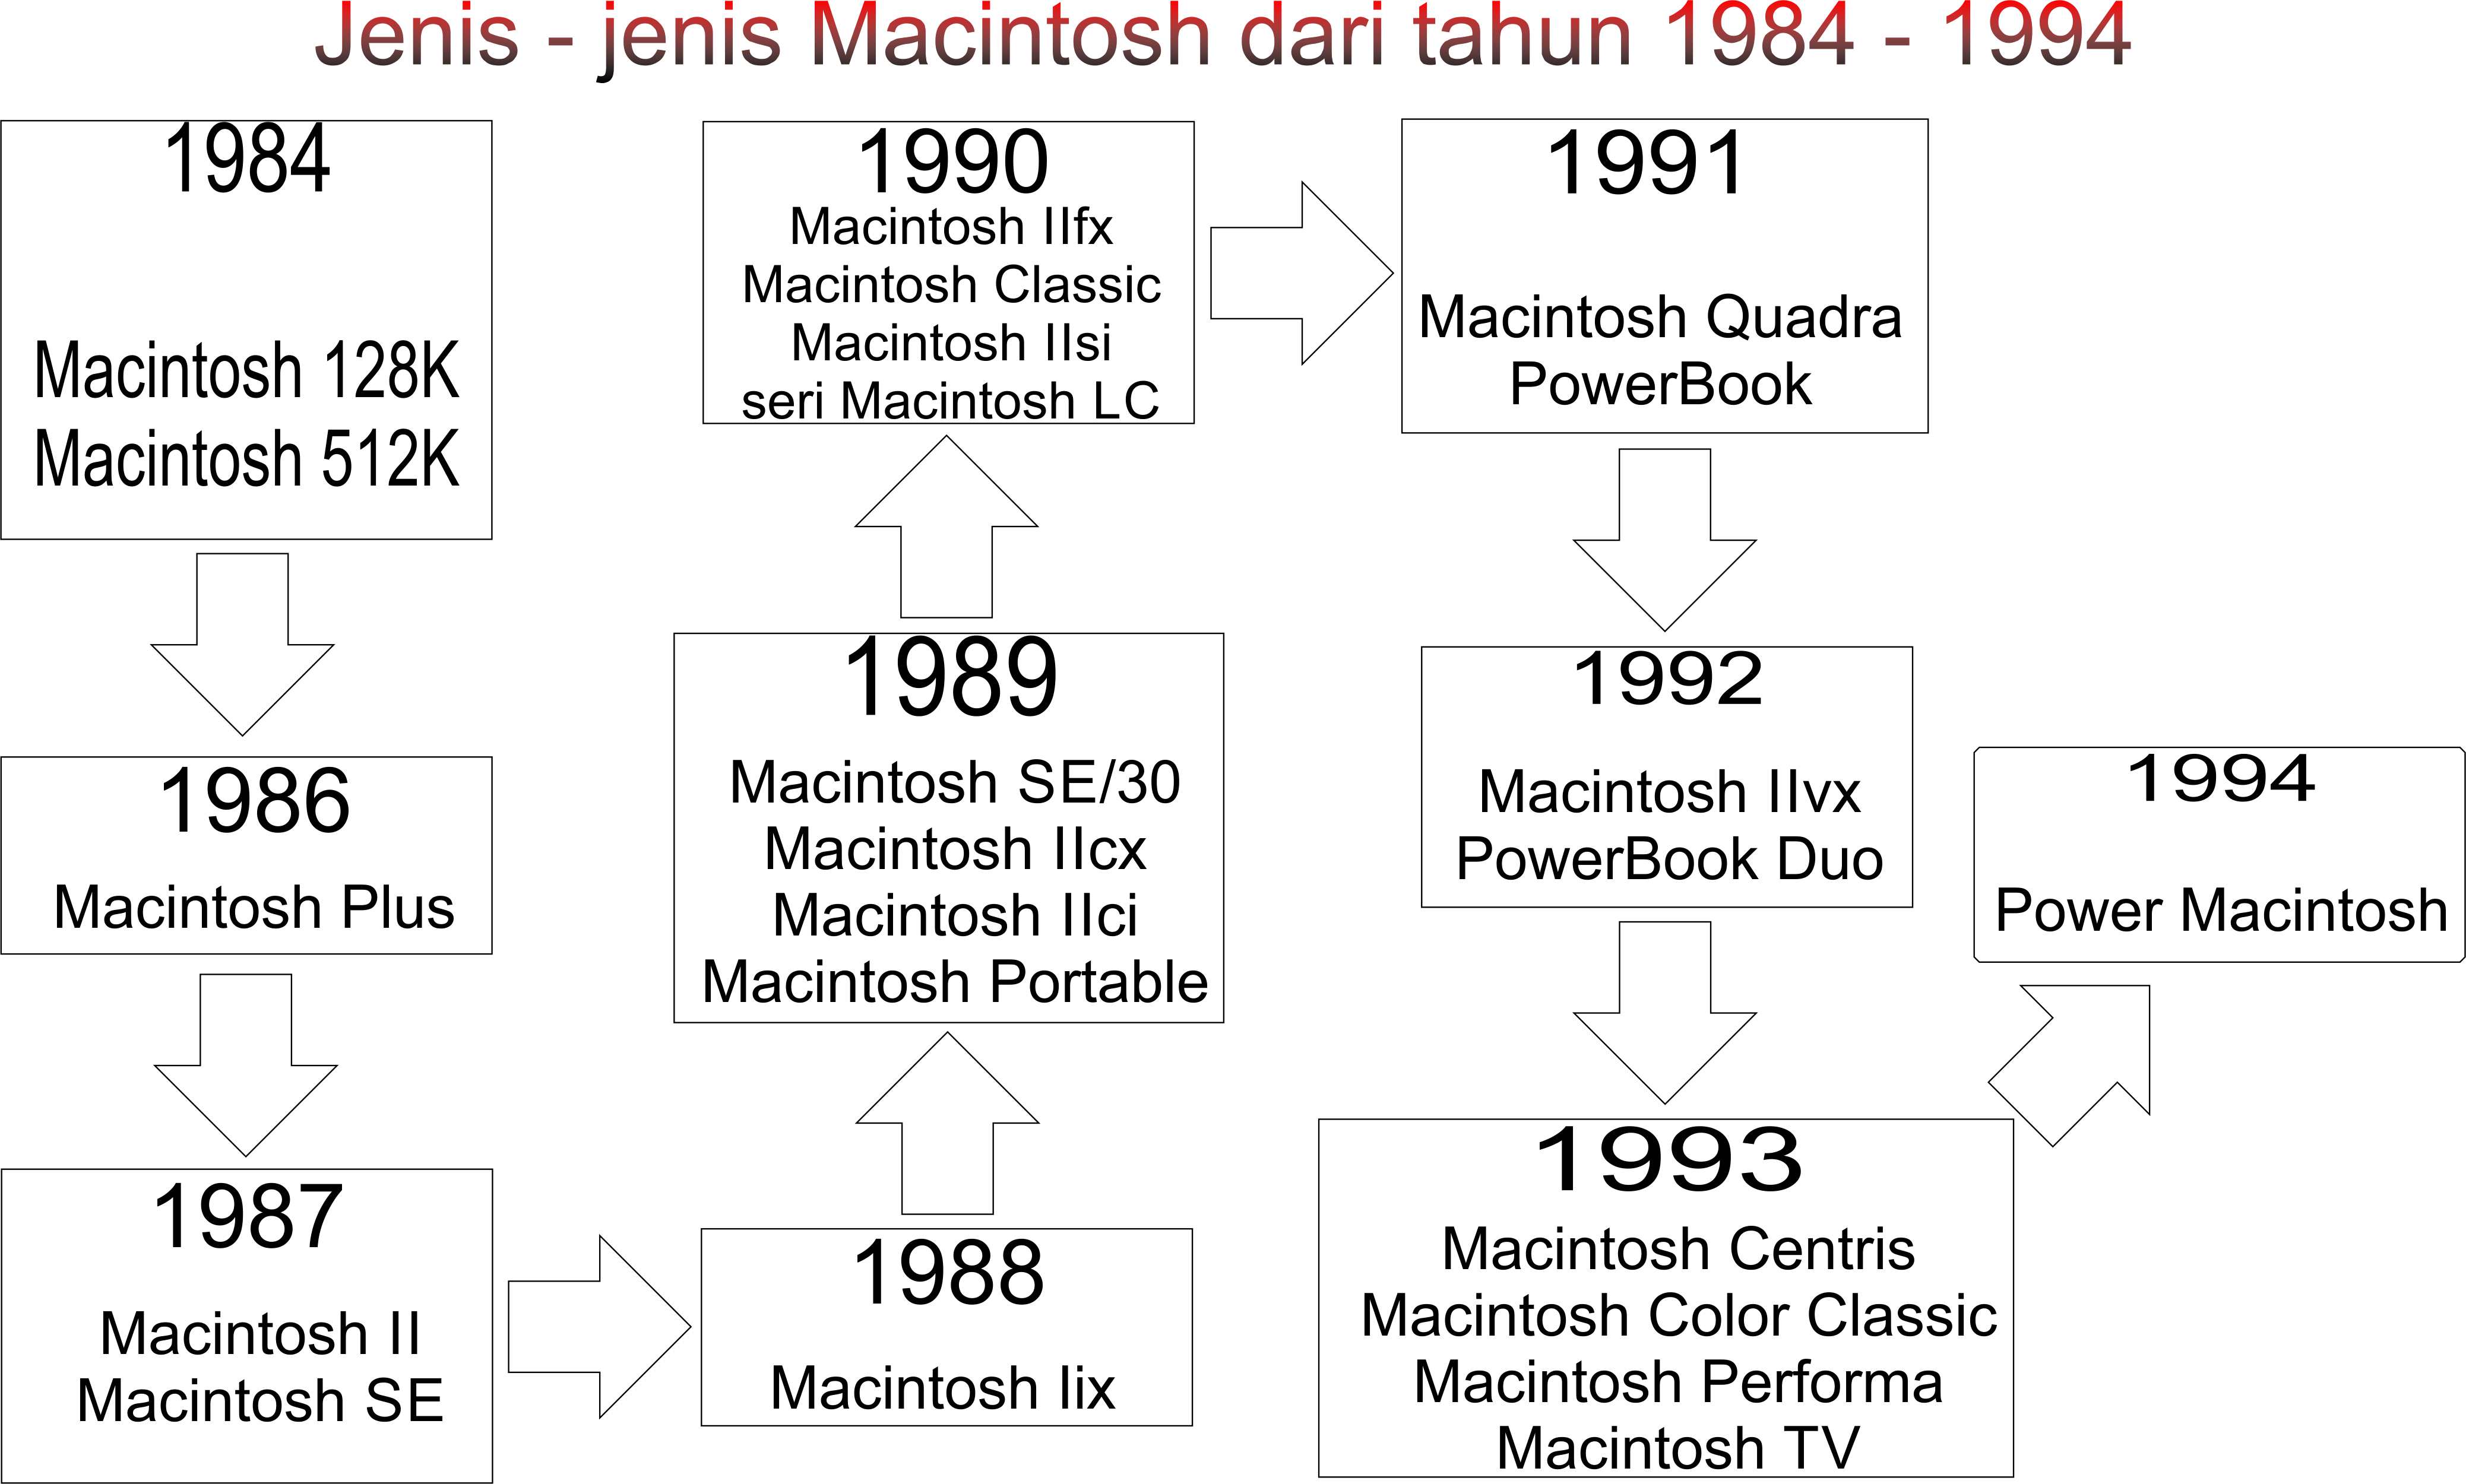
\includegraphics[width=1\textwidth]{figures/Gambar1.JPG}}
	\caption{JenisJenisMacintosh1984-1994.}
	\label{Gambar1}
	\end{figure}

	\ref{Gambar2}
	\begin{figure}[ht]
	\centerline{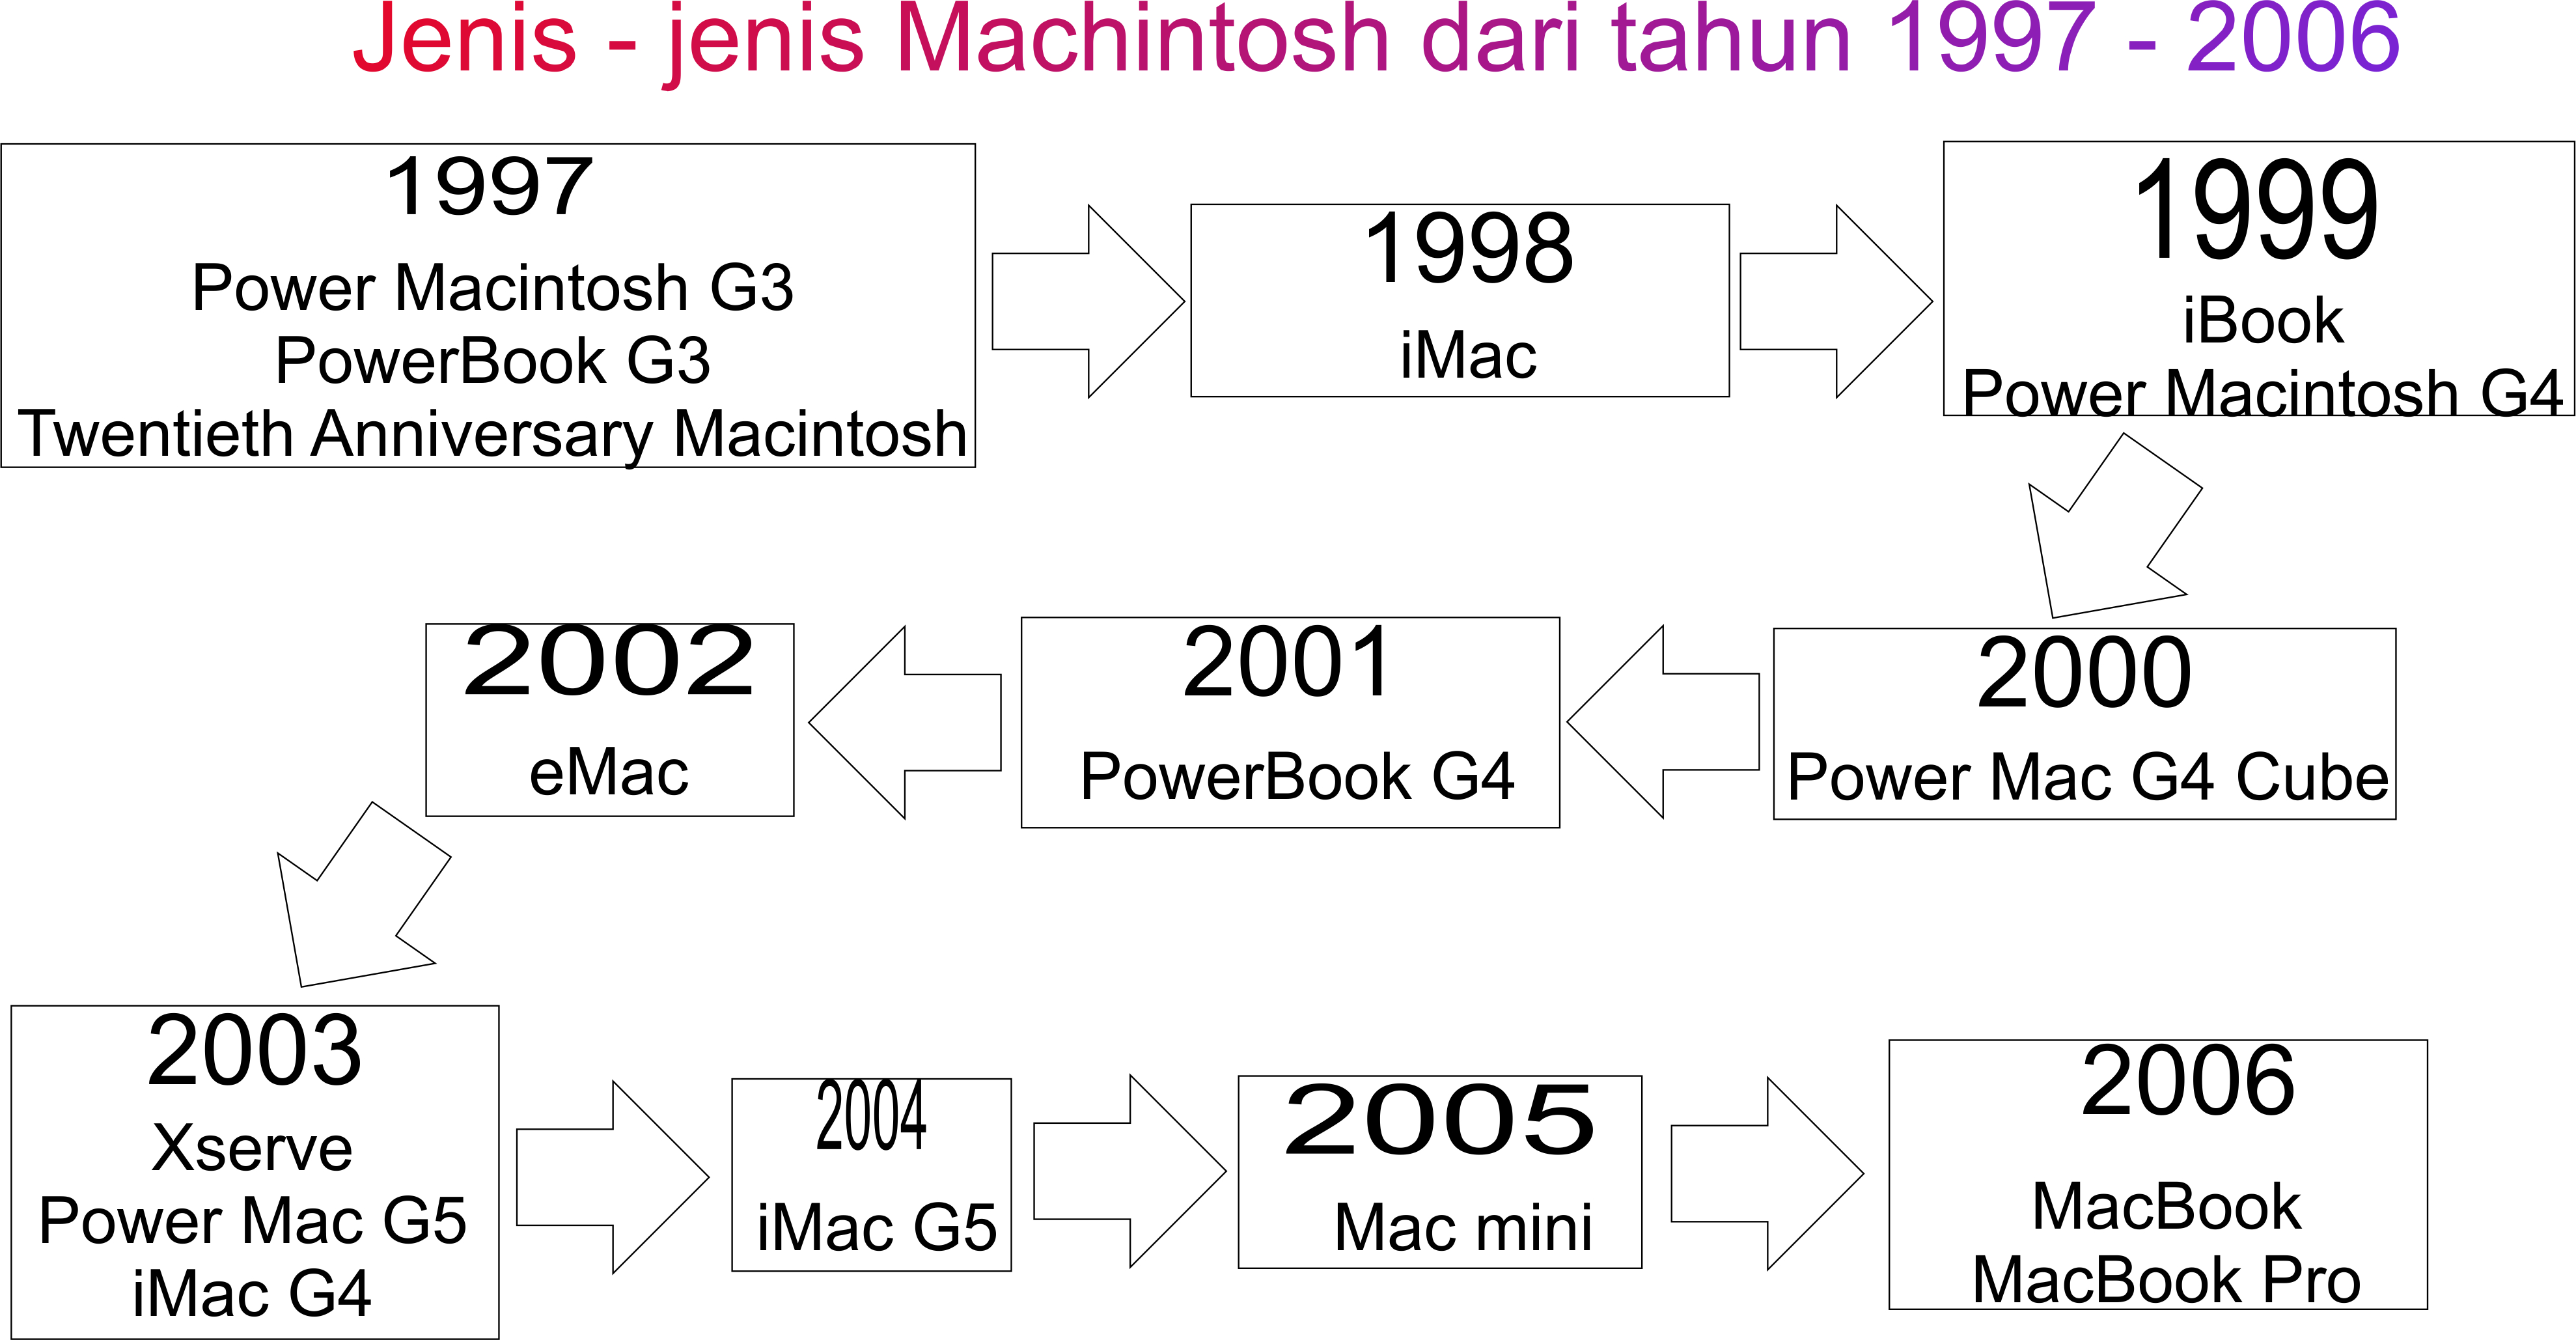
\includegraphics[width=1\textwidth]{figures/Gambar2.JPG}}
	\caption{JenisJenisMacintosh1997-2006.}
	\label{Gambar2}
	\end{figure}

\section{kelebihan dan kekurangan}
Adapun kelebihan dan kekurangan yang dimiliki system operasi Mac OS ini adalah sebagai berikut :

	\subsection{kelebihan}
	-Tampilan yang lebih glossy sehingga bagus untuk desain grafik/multimedia. 
	-Tidak mudah terserang virus, Karena dirancang oleh security oriented. 
	-Machintosh Mempunyai filtur yang bernama “sherlock“ yang fungsinya untuk mencari file pada harddisk dan dalam jaringan lokal, tetapi juga di Internet. 
	-High Performance khususnya untuk MAC OS X yang dapat untuk melakukan semua hal dalam menjalankan aplikasi dengan kecepatan baik. 

	\subsection{kelemahan}
	-Software untuk OS ini belum begitu lengkap seperti pada windows. 
	-Harganya masih terlalu mahal. 
	-Seakan hanya ditujukan untuk desainer grafis. 
	-Kurang cocok untuk aplikasi server dan game. 

Dalam sebuah artikel menyebutkan kekurangan dan kelebihan Mac OS
\cite{linuxwindows}

\section{The Real Leadership Lessons of Steve Jobs}
Enam bulan setelah kematian Jobs, penulis buku biografi terlarisnya mengidentifikasikan praktik yang dapat dicoba oleh setiap CEO.
Steve Jobs mendirikan Apple di garasi orang tuanya pada tahun 1976, digulingkan pada tahun 1985, kembali untuk menyelamatkannya dari kebangkrutan pada tahun 1997, 
dan pada saat dia meninggal, pada bulan Oktober 2011, telah membangun Ini menjadi perusahaan paling berharga di dunia. Sepanjang jalan ia membantu mengubah tujuh industri: 
komputasi personal, film animasi, musik, telepon, komputasi tablet, toko ritel, dan penerbitan digital. Dengan demikian dia termasuk dalam jajaran inovator hebat Amerika, 
bersama Thomas Edison, Henry Ford, dan Walt Disney. Tak satu pun dari orang-orang ini adalah orang suci, tapi lama setelah kepribadian mereka dilupakan, sejarah akan mengingat 
bagaimana mereka menerapkan imajinasi terhadap teknologi dan bisnis. Dalam bulan-bulan sejak biografi Jobs saya keluar, banyak komentator telah mencoba menarik pelajaran manajemen darinya. 
Beberapa dari pembaca itu memiliki wawasan, tapi saya pikir banyak dari mereka (terutama mereka yang tidak memiliki pengalaman kewiraswastaan) tetap mempertahankan sisi kepribadiannya yang kasar. 
Inti dari Jobs, menurut saya, adalah bahwa kepribadiannya adalah bagian integral dari caranya berbisnis. Dia bertindak seolah aturan normal tidak berlaku baginya, dan semangat, intensitas, dan emosionalisme
ekstrim yang ia bawa ke kehidupan sehari-hari adalah hal-hal yang juga dituangkan ke dalam produk yang ia buat. Kelesuan dan ketidaksabarannya merupakan bagian tak terpisahkan dari kesempurnaannya. 
Salah satu terakhir kali saya melihatnya, setelah saya selesai menulis sebagian besar buku ini, saya bertanya lagi tentang kecenderungannya untuk bersikap kasar pada orang lain. \"Lihatlah hasilnya\" 
jawabnya. \"Semua ini adalah orang-orang pintar yang bekerja sama, dan mereka bisa mendapat pekerjaan terbaik di tempat lain jika mereka benar-benar merasa brutal. Tapi mereka tidak melakukannya. 
\"Kemudian dia terdiam beberapa saat dan berkata, dengan sangat sedih\" Dan kami mendapatkan beberapa hal menakjubkan. \"Memang, dia dan Apple memiliki serangkaian hit 
selama belasan tahun terakhir yang lebih besar daripada perusahaan inovatif lainnya di zaman modern: iMac, iPod, iPod nano, Toko iTunes, Toko Apple, MacBook, iPhone, iPad, App Store, 
OS X Lion-tidak untuk
sebutkan setiap film Pixar. Dan saat dia melawan penyakit terakhirnya, Jobs dikelilingi oleh kader rekan yang sangat setia yang telah terinspirasi olehnya selama bertahun-tahun dan istri, 
saudara perempuan, dan empat anak yang sangat mencintai. Jadi saya pikir pelajaran nyata dari Steve Jobs harus diambil dari melihat apa yang sebenarnya dia capai. Saya pernah bertanya 
kepadanya apa pendapatnya tentang ciptaannya yang paling penting, mengira dia akan menjawab iPad atau Macintosh. Sebaliknya dia bilang itu milik Apple perusahaan. Membuat perusahaan 
yang abadi, katanya, jauh lebih sulit dan lebih penting daripada membuat produk hebat. Bagaimana dia melakukannya? Sekolah bisnis akan mempelajari pertanyaan itu satu abad dari sekarang. 
Inilah yang saya anggap kunci suksesnya.
Artikel ini menyebutkan tentang cara kepemimpinan Steve job \cite{isaacson2012real}.

\section{Kesimpulan}
Jadi kesimpulan dari artikel mengenai Macintosh atau MacOS yang telah dapat kita rasakan dari awal kemunculannya pada tahun 1984 hingga saat ini pada tahun 2017 MacOS memiliki 2 jenis yaitu Jenis Mac OS Classic (Klasik) dan Mac OS X sudah Berkembang menjadi banyak Series seperti yg pertama di keluarkannya yaiu System 1, System 2,3,\& 4 hingga yg terakhir dalam MacOS Klasik yaitu MacOS 9 pada tahun 1999. Dan juga dari Mac OS X yang hingga kini dapat kita peroleh dan rasakan mulai dari MacOS X 10.0 dengan nama lain yaitu \"Cheetah\" pada tahun 2001 hingga yang paling terbaru yaitu versi terbaru atau revisian dari Mac OS versi 10.12 yaitu Sierra dengan nama dan serial baru yaitu \"High Sierra\" dengan nomor seri 10.13 yang baru saja rilis pada 2017 ini

\chapter[Free BSD]
{Software\\ bsd}
% Nama Kelompok : FreeBSD
% Kelas         : D4 Teknik Informatika 1A
% Anggota       :
% 1. Jeremia Wahyudi Sianturi		1174029
% 2. Dwiyulianingsih				1174009
% 3. Arjun Yuda Firwanda			1174008
% 4. Dwi Septiani Tsaniyah			1174003
% 5. Ervanda Rambu Anarky			1174007
% 6. Muh. Rifky	Prananda			1174017
\section{FreeBSD}
	FreeBSD adalah suatu sistem operasi bersifat open source bertipe UNIX bebas yang diturunkan dari UNIX AT\&T lewat cabang Berkeley Software distribution
	BSD. FreeBSD adalah salah satu keluarga BSD yang saat ini banyak digunakan dan dikembangkan pada berbagai kalangan individu,
	perusahaan, dan bahkan universitas. Bila dibandingkan dengan windows FreeBSD relatif lebih sulit dalam penggunaannya, karenya masih bersifat text base
	dalam memberikan command sedangkan windows memiliki GUI yang jauh lebih dibandingkan FreeBSD keunggulan FreeBSD dibanding windows
	adalah kebebasan dalam penggunaannya bahkan pengembangan dari sistem operasi tersebut lisensinya sudah dijamin untuk kebebasan.
	FreeBSD mengoptimalkan penggunaan flatform PC. FreeBSD menyediakan kemudahan dalam penggunaan instalasi dan dukungan yang luas terhadap perangkat keras dalam PC.
	FreeBSD mendukung arsitektur i386 dan Alpha, dan pengembangannya pada beberapa flatform telah dilakukan.
	\ref{index} 
	\begin{figure} [ht]
	\centerline{
\includegraphics[width=1\textwidth]{figures/index.jpg}}
	\caption{gambarindex}
	\label {index}
	\end {figure}
\subsection{Sejarah}
	menurut \cite{luanmembangun} menyebutkan bahwa :
	Berkeley software distribution diawali dari modifikasi AT\&T Unix software, sebelum berkembang menjadi suatu proyek yang signifikan. Namun sayangnya, AT\&T masih memegang lisensi untuk UNIX dan bertentangan dengan Berkeley Software Design Inc. BSDI yang mengklaim bahwa Berkeley Software Distribution juga termasuk source code AT\&T.
	Kasus lisensi ini sempat dibawa ke pengadilan, dan diproses yang kemudian  menghasilkan bahwa Bill Jolitz berwenang untuk mengambil bagian dari software yang bukan berasal dari AT\&T dan kemudian mengembalikannya menjadi free UNIX. Ini merupakan sebuah awal baru dari lahirnya modern BSD.
	Dalam pengembangannya FreeBSD melibatkan begitu banyak pihak yang notabene merupakan programmer individu berkemampuan tinggi yang dikenal sebagai commiters. Commiters ini dipilih oleh FreeBSD core team dan memiliki wewenang langsung untuk melakukan suatu perubahan-perubahan pada system yang  berjalan.
	FreeBSD lahir pada tahun 1992 saat Jordan K. Hubbard, Rob Grimes, dan Nate Williams merilis sebuah paket yang dikenal dengan unofficial 386BSD patchkit. Dari sana lahirlah suatu mekanisme yang membentuk 386BSD 0.5 1/2, akan tetapi pada 1993 Jolitz mencabut persetujuan pada proyek tersebut dan melahirkan FreeBSD. 
	Jordan K Hubbard dan David Greenman kemudian membentuk suatu kerjasama untuk mempersiapkan sebuah proyek CDROM FreeBSD versi 1.0 berbasis Net/2 yang telah dirilis pada bulan desember tahun 1993, setelah itu pada bulan November 1994 versi kedua dari FreeBSD dirilis yaitu versi 2.0 yag tidak lagi 
	berbasis Net/2 tetapi telah diupgrade menjadi berbasis 4.4BSD BSD dibuat, dikembangkan serta digunakan secara bebas sebagai perlawanan terhadap lisensi UNIX yang dimiliki oleh AT\&T. oleh karena itu BSD mempunyai lisensi sendiri yang memungkinkan setiap individu bebas melakukan pengembangan dan
	FreeBSD telah digunakan diseluruh penjuru internet oleh beberapa perusahaan yang memiliki orientasi pada internet. sebagai contohnya saat ini the \"babybell\" US west menggunakan FreeBSD untuk menjalankan operasional internet. IBM, Nokia, dan banyak perusahaan hardware menggunakan FreeBSD pada embedded system.
	dalam kenyataannya jika sebuah perusahaan serius untuk melakukan manajemen bandwich internet, kemungkinan besar sistemnya menjalankan FreeBSD.
	saat ini FreeBSD memiliki hampir 300 developer. comitters mempunyai hak read-and-write atas master source code dan dapat men-develop, debug, atau memperbaiki kulaitas bagian yang dianggap penting.
	sebagai contoh, developmen networking dibahas dalam milis-milis yang banyak tersebar di media sosial ada pula beberapa chanel IRC untuk mendiskusikan banyak hal mengenai FreeBSD.
	para committers bertanggung jawab agar FreeBSD tetap berjalan dan memabah fitur baru serta mengevaluasi patch yang dikirim oleh para kontributor. 
	hingga akhirnya FreeBSD memiliki users yang jauh lebih banyak karena kita dapat mendownload keseluruhan FreeBSD dengan gratis dan tidak perlu register, upgrade atau mengirim email ke mailing list.

\subsection{VarianFreeBSD}
	Varian dari FreeBSD kami mendapatkan referensi dari \cite{nugroho2015analisis} yang kami kembangkan menjadi :
	FreeBSD memiliki dua versi saat dirilis. versi tersebut antara lain versi-CURRENT dan versi-STABLE. selain itu varian FreeBSD juga ada UNIX FreeBSD, NETBSD, OpenBSD, UNIX lainnya, dan AIX yang dikenal dapat dijalankan pada banyak jenis arsitektur, dan FreeBSD yang mendukung flatform X86, AMD64, IA64, SPARC64, dan Alpha.
	FreeBSD 6.0 dikenal dengan stabilitas, performa, dan keamannanya sehingga digunakan oleh banyak perusahaan di seluruh dunia. rilis UNIX freeBSD yang digunakan saat ini adalah versi 6.2. 
	Sebenarnya masih banyak lagi jenis-jenis sistem operasi yang dapat dikatakan berbasis dengan FreeBSD seperti IRIX, HPUX, LINUX, Sun Solaris, Mac OS X, BSD/OS dan juga masih ada lagi yang belum disebutkan tapi mungkin karena berikut merupakan kesimpulan sederhana jadi tidak dijelaskan secara semua atau dapat dikatakan menyeluruh. 
	Jadi dapat ditarik bahwa banyak jenis-jenis dari OS FreeBSD yang telah disebutkan.
	pengembangan gentoo/FreeBSD menggunakan versi ini, sedangkan  pengembangan dengan versi lama telah dihentikan dan tidak lagi didukung. pada varian BSD NETBSD dan OPENBSD memiliki modal pengembangan sistem operasi yang terbuka akan tetapi memiliki susanan tertentu yaitu :
	1. contributor, adalah developer yang menulis kode, patch atau dokumentasi, akan tetapi tidak memiliki hak untuk menulis atau membuat suatu file dalam source tree. jika pekerjaan yang mereka lakukan ingin dimasukkan maka harus diperiksa terlebih dahulu oleh committers atau dengan persetujuan beberapa orang committers
	2. commiters adalah developer yang memiliki hak menulis dan mengakses source tree, dalam lingkup cvs, memiliki hak commit secara tipikal dan hanya bekerja dalam bagian terpilih di suatu proyek.
	3. coreteam memiliki wewenang untuk membimbing secara keseluruhan arah dan tujuan proyek, dan membuat keputusan akhir dalam kasus berselisih paham antar developer mengenai source code atau hal-hal lain. OpenBSD tidak memiliki coreteam secara formal namun Theo De Raadt bertugas sebagai pemimpin proyek.
	setap orang dapat menjadi contributor dengan mengirimkan patch atau membenarkan kesalahan penulisan dalam sebuah halaman manual orang yang mengkontribusikan banyak hal, atau berkompeten dalam suatu proyek akan dipeomosikan menjadi commiters yang ditujukan untuk menjaga committers yang lain memeriksa terlalu banyak hal dalam waktu yang sama.
\subsubsection{versi-CURRENT}
	versi-CURRENT merupakan versi yang pertama kali dirilis biasanya versi ini dipakai oleh para develover yang sudah mahir mengenai
	cara kerja dari FreeBSD agar dapat menemukan berbagai bugs paska produksi. setelah versi-CURRENT diperbaiki maka versi tersebut
	akan menjadi versi stable yang siap digunakan karena dalam versi-CURRENT kurang familiar bagi pengguna baru FreeBSD.
	\ref{freebsd} 
	\begin{figure} [ht]
	\centerline{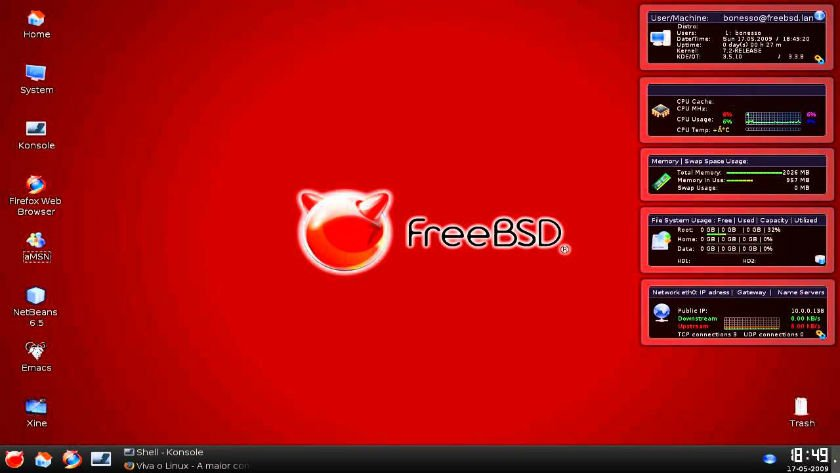
\includegraphics[width=1\textwidth]{figures/freebsd.jpg}}
	\caption{gambarindex}
	\label {freebsd}
	\end {figure}
\subsection{Sejarah}
\subsubsection{versi-STABLE}
	versi-STABLE adalah versi pengembangan ddari versi sebelumnya yaitu versi-CURRENT yang dianggap kurang familiar.
	versi-STABLE siap digunakan oleh siapapun yang baru mencoba FreeBSD karena versi sebelumnya hanya ditujukan kepada
	orang yang mahir dalam mengidentivikasi masalaah yang muncul pada versi tersebut.
\subsubsection{NETBSD}
	NetBSD dapat juga dikatakan mirip dengan FreeBSD dalam berbagai macam bentuk dan aspek. Kedua proyek ini saling berbagi source code dan developer. 
	Tujuan paling utama dari NetBSD adalah membuat sistem operasi yang dapat diporting ke berbagai macam plattform hardware. 
	Sebagai contohnya bahwa NetBSD dapat berjalan di berbagai macam plattform hardware yaitu : bahwa NetBSD dapat berjalan di VAXes, PocketPC, Alpha server, dan Compaq iPaq. Bahkan NetBSD dapat berjalan juga pada hardware yang belum ada (belum diluncurkan). 
	Source code NetBSD diberikan secara bebas, sama seperti pendahulunya, FreeBSD.
\subsubsection{openBSD}
	OpenBSD merupakan cabang dari NetBSD mulai tahun  1996, tujuan utam dari OpenBSD adalah membuat OS BSD yang aman. 
	OpenBSD adalah BSD yang pertama kali men-suport hardware-accelerated crytography {membolehkan untuk men-encrypt dan decrypt informasi pada waktu yang singkat, para developenya sangat bangga karena faktanya, default instalasi OpenBSD tidak dapat di-hack selama kira-kira 4 tahun.
\subsubsection{UNIXFreeBSD}
	FreeBSD dapat dikatakan mirip dengan sistem operasi Unix yang bebas {berlisensi}. Pada tahun 1993 ketika pengembangan 386BSD dihentikan, maka lahirlah dua proyek baru yang satu dikenal dengan nama Net BSD, yang dikenal dapat dijalankan pada banyak jenis arsitektur, 
	dan yang satunya lagi dikenal dengan sebutan FreeBSD yang mendukung platform x86, amd64, ia64, sparc64 dan alpha. 
	Free BSD 6.0 dikenal juga denagn stabilitas, performa dan keamanannya sehingga sering digunakan oleh perusahaan-perusahaan terkenal yang ada di seluruh dunia. 
	Saat ini unix FreeBSD yang digunakan adalah versi 6.2. Dan sebentar lagi juga akan keluar pengembangan  Gentoo/FreeBSD versi terbaru, sedangkan versi lama yang ingin dikembangkan malah diberhentikan proyeknya dan tidak didukung sama sekali pembentukannya. 
	Pasti kita semua bertanya-tanya apa itu Gentoo/FreeBSD? Baiklah akan dijelaskan bahwa Gentoo/FreeBSD adalah subproyek dari proyek Gentoo/Alt, Yang tujuannya hanya untuk menyediakan sistem operasi FreeBSD berkemampuan penuh dengan mengambil rancangan dari Gentoo Linux, seperti sistem unit dan sistem manajemen paket Portage.
\subsubsection{UNIXLainnya}
	Masih ada beberapa UNIX OS di luar sana, beberapa bahkan menyewa nama trademark dari UNIX sehingga mereka dapat menyebut diri mereka itu UNIX
\subsubsection{AIX}
	Salah satu pesaing ketat dari UNIX adalah IBM AIX. AIX mengklaim bahwa mereka mempunyai journaling filesystem terbaik seperti, mampu mencatat seluruh disk transaction yang terjadi, sehingga mereka mampu me-recover system tanpa banyak masalah kemampuan ini meningkatkan reliability. 
	Dan AIX juga berbasis BSD.
\subsection{Tujuan}
	Tujuan dari adanya software ini adalah untuk menyediakan software yang tentu saja dapat digunakan dalam berbagai kepentingan dengan mudah dan gratis (free). karena software ini disediakan dengan gratis dan dapat digunakan oleh siapa saja termasuk untuk meraih kepentingan komersil, 
	source kode yang tersedia dengan gratis siapun dapat meningkatkan  peforma melalui free bsd ini atau memungkinkan bug mensubmit source codenya dan dapat digunakan sesuai dengan keinginan si pengguna.
	Tujuan dari adanya versi-CURRENT dan versi-STABLE adalah untuk memberitahukan fixed bugs bagi para pengguna
	dan meyakinkan pengguna dengan fitur - fitur terbaru dan masalah yang telah diatasi. selain perbedaan diantara versi-CURRENT dan versi-STABLE
	pemberian nama dari versi-STABLE juga telah dibuat sedemikian rupa hingga para penggguna tahu  perbaikan - perbaikan yang telah dilakukan.
\subsection{kegunaanFreeBSD}
	pada saat ini FreeBSD dikenal sebagai network administrator operating system karena FreeBSDberjalan dengan cepat dan telah banyak tersedia berbagai networking tools. selain itu, FreeBSDdapat berjalan denngan cepat dan efisien didalam sebuah laptop untuk menjalankan aplikasi perkantoran, atau sebagai email client maupun email database.
	instalasi dari FreeBSD dapat dikatakan cukup mudah bagi yang sudah pernah menginstall system operasi windows.
\subsection{keuntungandankelemahan}
	keuntungan dan kelemahan kami mengambil referensi dari : \cite{nugroho2015analisis}
	keuntungan :
	1. FreeBSDdapat berjalan lebih cepat daripada LINUX dalam beberapa bagian misalnya sebagai server NFS
	2. dalam aplikasi server secara prinsip BSD sama baiknya dengan LINUX
	kelemahan :
	1. FreeBSD tidak dapat digunakan pada microkanal lama
	2. FreeBSD tidak dapat mendukung ISA-plug-and-play-card
	3. FreeBSD tidak bisa menandingi perkembangan LINUX yang cepat karena kurangnya developer
	4. FreeBSD belum jelas masa depannya untuk server database
\subsection{Kesimpulan}
	Dari penjelasan diatas dapat disimpulkan bahwa FREEBSD mempunyai banyak fitur-fituryang dapat dipelajari satu per satu. Dan ada kelebihan, kekurangan yang ada di FREEBSD, diataranya banyaknya tersedia aplikasi dan program file gratis. 
	Mudah di kustomisasi atau dapat dirubah-rubah secara bebas. Freebsd mempunyai fitur multiuser, bersifat opensource, memiliki sistem software third-party yang memberikan kemudahan yang berarti bagi para user untuk menambah atau menghapus aplikasi-aplikasi.
	Para user cukup mengeksekusi satu baris perintah dan aplikasi-aplikasi dengan sendirinya di download dan diinstal secara otomatis, sehingga tugas-tugas didalam system Freebsd menjadi mudah dan praktis. 
	Dari beberapa kelebihan diatas secara progaming Freebsd dapat dikatakan system yang dapat mempermudah user dalam menggunakan dalam berbagai tugas-tugas system operasi.
	Di dalam Freebsd terdapat kekurangan juga, diantaranya relatif penggunaannya sulit karena masih dalam bentuk text base dalam mengcommandnya, artinya dalam memerintahnya masih sulit. Tidak mendukung ISA plug and play chard, artinya tidak dapat memasang dan memainkan. 
	Kecilnya basis developer dan pemakai yang mencari bug/kelemahan program.
	Operating sistem ini dinamakan freeBSD karena software ini gratis untuk digunakan oleh siapapun termasuk untuk kepentingan komersial, source code yang tersedia dengan gratis, siapapun dapat meningkatkan performa freeBSD ini atau menemukan bug
	(Pengertian bug adalah kesalahan pada komputer baik disebabkan oleh perangkat lunak ataupun perangkat keras sehingga komputer tidak bekerja dengan semestinya ) untuk mensubmit souce codenya, kata ‘free’ dapat diartikan sebagai gratis, atau dapat digunakan sesuai keinginan user.
	FreeBSD dikenal sebagai network administrator operating system karena FreeBSD berjalan dengan cepat dan telah banyak tersedia berbagai networking tools. 
	selain itu, FreeBSD dapat berjalan denngan cepat dan efisien didalam sebuah laptop untuk menjalankan aplikasi perkantoran, atau sebagai email client maupun email database.
	FreeBSD dapat dikatakan cukup mudah bagi yang sudah pernah menginstall system operasi windows.
	FreeBSD dapat berjalan di personal komputer yang menggunakan sistem arsitektur Intel. Artinya dapat mendapatkan secara gratis tanpa berbayar.


%\chapter[Android]
%{Software\\ android}
%\input{chapter/android.tex}

\part[Hardware dan Networking]
{Arsitektur Komputer\\ Hardware}

%\chapter[Sejarah Computer]
%{Hardware\\ computer}
%\input{chapter/computer.tex}

%\chapter[CPU atau Prosesor]
%{Hardware\\ CPU}
%\input{chapter/cpu.tex}

%\chapter[Input Output Device]
%{Hardware\\ io}
%\input{chapter/io.tex}

%\chapter[Memori]
%{Hardware\\ Memori}
%% Nama Kelompok : Linux
% Kelas : D4 TI 1A
% 1. Kadek Diva Krishna Murti (1174006)
% 2. Duvan Silalahi (1174011)
% 3. Oniwaldus (1174005)
% 4. Choirul Anam (1174004)
% 5. Sri Rahayu (1174015)
% 6. Ilham Habibi (1174028)


\begin{figure}[ht]
\centerline{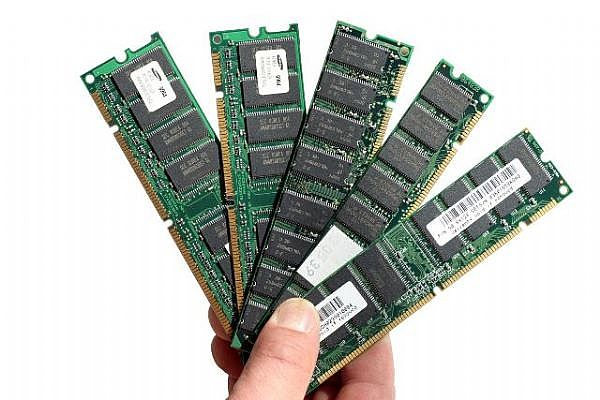
\includegraphics[width=1\textwidth]{figures/memori.jpg}}
\caption{Contoh gambar memori.}
\label{memori}
\end{figure}

Memori disebut juga sebagai memori fisik merupakan suatu istilah generik yang merujuk pada media penyimpanan data sementara pada komputer. Setiap program dan data yang sedang diproses oleh prosesor akan disimpan di dalam memori fisik. Data yang disimpan pada memori fisik bersifat sementara, karena data yang disimpan di dalamnya akan tersimpan selama komputer tersebut masih dialiri daya dengan kata lain, komputer itu masih dalam keadaan hidup. Ketika sebuah komputer dimatikan atau direset, data yang disimpan dalam memori fisik akan hilang. Oleh sebab itulah sebelum anda mematikan komputer Anda, anda harus benar - benar menyimpan semua data yang belum anda simpan ke media penyimpanan permanen umumnya berbasis disk, seperti hard disk atau floppy disk, sehingga pada saat komputer anda dihidupkan kembali data tersebut dapat dibuka kembali di lain kesempatan. Memori fisik biasanya diterapkan dalam bentuk Random Access Memory (RAM), yang bersifat dinamis (DRAM). Disebut Random Access adalah karena akses terhadap tempat-tempat di dalamnya dapat dilakukan secara acak atau random, bukan secara berurutan atau sekuensial. Meskipun demikian, kata random access dalam RAM ini sering terjadi salah paham. Sebagai contoh, memori yang hanya dapat dibaca seperti Read Only Memory (ROM) juga bisa diakses secara random, tetapi ia dibedakan dengan RAM karena ROM dapat menyimpan data tanpa kebutuhan daya dan tidak dapat ditulisi sewaktu-waktu. Tidak hanya itu, hard disk sebagai media penyimpanan juga bisa diakses secara random, namun hardisk tidak dikategorikan kedalam sebuah khusuRandom Access. Ini adalah contoh gambar memori \ref{memori}

\section{Sejarah Memori}
Perkembangan micro computer atau yang biasanya sering disebut juga dengan nama PC (Personal Computer) yang sedemikian pesat tentunya tidak lepas dari kebutuhan manusia akan informasi yang harus diolah oleh PC. Perkembangan teknologi tersebut termasuk dalam teknologi perangkat keras, perangkat lunak, serta fungsi atau algoritma yang digunakan dalam memproses informasi yang diolah tersebut.
Pada awal ditemukannya PC banyak orang menganggap PC sebagai barang yang mahal atau mewah, namun kini anggapan itu tidak berlaku lagi karena hampir semua orang sudah memilikinya. Bisa dikatakan, orang yang tidak mengenal komputer pada zaman sekarang akan dicap sebagai orang yang gagap teknologi. Jika pada saat itu PC yang diotaki oleh prosessor Intel 8088 hanya mampu berjalan dengan kemampuan kecepatan 4,77 MHz yang digunakan untuk menajalankan program pengolah kata dalam pembuatan dan mengubah dokumen, spreadsheet sederhana untuk mengerjakan pekerjaan akuntansi maupun bisnis, dan program database sederhana serta sedikit program pendidikan dan game yang juga masih sangat sederhana. Pada masa sekarang PC yang diotaki Intel Pentium 4 mampu berjalan dengan kecepatan 2GHz, bahkan baru - baru ini Intel Corp melalui ajang Intel Developer Forum-nya, telah menunjukkan demo prosessor Intel berkecepatan 3,5GHz Suatu penemuan teknologi yang cukup fantastis dan muktakhir. Namun pada perkembangan selanjutnya kemampuan PC tidak selalu ditentukan oleh perkembangan prosessor semata, bisa juga faktor lainnya, seperti teknologi chipset, memori, kartu VGA, perangkat media simpan, dan sebagainya. Semua perangkat saling berevolusi dan berkembang ke arah yang lebih baik untuk bersama - sama membangun suatu sistem PC yang tangguh. Perkembangan kemampuan prosessor yang begitu pesat tentunya harus diimbangi dengan peningkatan kemampuan memori. Memori dibutuhkan oleh prosessor sebagai tempat penyimpan data atau informasi sekaligus sebagai penyimpan hasil dari perhitungan yang dilakukan oleh prosessor itu sendiri, sehingga kemampuan memori dalam mengelola data tersebut sangatlah penting. Percuma saja apabila kita memliki sebuah sistem PC dengan prosessor berkecepatan tinggi apabila tidak diimbangi dengan kemampuan memori yang sepadan. Ketidaktepatan dalam perpaduan kemampuan prosessor dengan memori dapat menyebabkan inefisiensi bagi keduanya. Andaikan apabila kita mempunyai sebuah prosessor yang mampu mengelola arus data sebanyak 100 instruksi per detiknya, sementara kita memiliki memori dengan kemampuan menyalurkan data ke prosessor sebesar 50 instruksi per detiknya. Yang terjadi adalah sistem akan mengalami ketidakseimbangan yang disebabkan perbedaan kecepatan kerja antara prosessor dengan memori yang berarti prosessor harus menunggu data dari memori dan menyebabkan data yang seharusnya dapat dikerjakan dalam waktu 1 detik, menjadi 2 detik karena kemampuan memori yang terbatas. 

\section{Penggunaan memori}
Komponen utama dalam suatu sistem komputer adalah Arithmetic and Logic Unit (ALU), Control Circuitry, Storage Space dan piranti Input atau Output. Tanpa adanya sebuah memori, sebuah komputer hanya akan berfungsi sebagai perangkat pemroses sinyal digital saja, contohnya kalkulator atau media player. Yang membuat sebuah komputer dapat disebut sebagai komputer multi-fungsi (general-purpose)  adalah kemampuan  dari memori untuk menyimpan data, instruksi serta informasi. Komputer merupakan sebuah piranti digital oleh karena itu, informasi yang disajikan oleh komputer yaitu menggunakan sistem bilangan biner atau binary. File yang berupa teks, angka, gambar, suara dan video akan dikonversikan menjadi sekumpulan bilangan biner atau binary digit atau disingkat bit. Sekumpulan bilangan - bilangan biner dikenal dengan istilah BYTE, dimana  1 bita sama dengan 8 bit, 1 bit sama dengan 1 karakter, 1 kilobita sama dengan 1024 bita, dan bps sama dengan bit per second, 1 kbps sama dengan 1000 bps, 1 mbps sama dengan 1.000.000 bps. Semakin besar suatu ukuran memori maka semakin banyak pula informasi yang dapat disimpan di dalam media penyimpanan komputer.

\section{Jenis - Jenis Memori}

\subsection{Jenis Memori Yang Populer}

Berikut ini beberapa jenis memori yang banyak digunakan pada saat ini sebagai berikut:

\begin{enumerate}

\item RAM (Random Acces Memory) adalah memory sebagai tempat penyimpanan sementara pada saat komputer di jalankan dan dapat di akses secara acak atau random. Fungsi dari RAM adalah mempercepat pemrosesan data pada komputer. Semakin tinggi jumlah RAM yang Anda miliki, semakin cepat pula kemampuan komputer Anda dalam mengeksekusi.
Jenis Memory RAM :

\begin{itemize}

\item EDORAM (Extended Data Out RAM)  
\item SDRAM (Synchronous Dynamic RAM)  
\item DDR SDRAM (Double Data Rate Synchronous Dynamic RAM) 
\item RDRAM (Rambus Dynamic RAM)

\end{itemize}	

\item Menurut artikel yang berjudul Evolusi Komputer, Kinerja Komputer Dan Interconnection Networks Dalam Perkembangan Dunia Teknologi Informatika menyebutkan bahwa Registers adalah media penyimpan internal CPU yang digunakan saat proses pengolahan data. Memori ini bersifat sementara, biasanya hanya digunakan untuk menyimpan data saat diolah ataupun data untuk pengolahan selanjutnya. Sistem dan bus yang menghubungkan komponen-komponen eksternal CPU dengan sistem lain, seperti memori utama serta piranti masukan atau keluaran dan juga menghubungkan komponen – komponen internal CPU dengan system lain, seperti Arimathics Logics Unit, Unit Control, dan Registers system koneksi dan bus tersebut disebut CPU Interconnections. \cite{junior2016evolusi}

\item Menurut artikel yang berjudul Evolusi Komputer, Kinerja Komputer Dan Interconnection Networks Dalam Perkembangan Dunia Teknologi Informatika menyebutkan bahwa Read Only Memory disingkat ROM merupakan memori yang tidak dapat dihapus isinya, hanya dapat dibaca, dan sudah diisi oleh pabrik pembuat komputer atau bisa dikatakan tidak bisa diprogram kembali. Sebagian perintah pada ROM akan dipindahkan ke RAM. Perintah yang ada di ROM antara lain, perintah untuk menampilkan pesan dilayar, perintah untuk membaca Sistem Operasi dari disk, dan perintah untuk mengecek semua peralatan yang ada di Unit Sistem.
Perkembangan ROM (Read Only Memory)
- Programble ROM disingkat PROM merupakan ROM yang bisa diprogram kembali dengan catatan hanya bisa diprogram 1 x.
- Re-Programble ROM disingkat RPROM merupakan ROM yang bisa diprogram ulang sesuai dengan yang kita inginkan.
- Eraseble Programble ROM disingkat EPROM merupakan ROM yang dapat dihapus dan diprogram kembali tetapi cara penghapusannya dengan menggunakan Sinar Ultraviolet.
- Electrically Eraseble Programble ROM disingkat EEPROM merupakan ROM yang bisa diprogram dengan Teknik Elektronik. \cite{junior2016evolusi}

\item Dynamic RAM disingkat DRAM merupakan salah satu jenis RAM yang harus disegarkan secara berkala oleh CPU supaya data yang terkandung di dalamnya tidak hilang. DRAM merupakan salah satu tipe RAM yang terdapat dalam PC.
Compmentary Meta-Oxyde Semiconductor disingkat CMOS merupakan jenis chip yang memerlukan daya listrik dari baterai. Chip ini berisi memori 64-byte yang isinya dapat diganti. Chip ini biasanya mengatur berbagai pengaturan - pengaturan dasar yang terdapat 
pada perangkat komputer, seperti piranti yang digunakan untuk memuat sistem operasi dan termasuk pula tanggal dan jam sistem. CMOS merupakan bagian dari ROM.

\item Sychronous Dynamic RAM disingkat SDRAM merupakan kelanjutan dari DRAM tetapi memiliki kecepatan yang lebih tinggi daripada DRAM dan telah disinkronisasi oleh clock sistem. DRAM ini cocok digunakan untuk sistem dengan bus yang memiliki kecepatan sampai 100 MHz.

\item Dual In-line Memory Module disingkatan DIMM dari  berkapasitas 168 pin, kedua belah modul memori ini aktif, setiap permukaan adalah 84 pin. Berbeda dengan SIMM yang berfungsi hanya pada sebelah modul saja. Mensuport 64 bit penghantaran data. SDRAM
(Synchronous DRAM) menggunakan DIMM dan merupakan penganti dari DRAM, FPM (fast Page Memory) dan EDO. SDRAM memiliki fungsi untuk mengatur (synchronizes) memori supaya setara dengan CPU clock supaya pemindahan data yang dilakukan dapat dilakukan secara cepat. Terdapat dalam dua kecepatan yaitu 100MHz (PC100) dan 133MHz (PC133). DIMM 168 PIN. DIMM merupakan jenis RAM yang populer dan paling banyak terdapat di pasaran.

\item Cache merupakan memori yang berkapasitas terbatas, namun memori ini memiliki kecepatan  yang tinggi dan lebih mahal dibandingkan memory utama. Cache ini terletak di antara register pemroses dan memori utama, dan memiliki fungsi agar pemroses tidak langsung mengacu kepada memori utama tetapi langsung di cache memory yang kecepatan aksesnya lebih tinggi, metode ini akan meningkatkan kinerja sistem. Cache memori merupakan salah satu tipe RAM tercepat yang pernah ada, dan digunakan oleh CPU, hard drive, dan beberapa pernah lainnya.

\item Magnetik Disk merupakan sebuah piringan bundar yang terbuat dari bahan tertentu seperti, logam atau plastik dengan permukaan dilapisi bahan - bahan yang dapat di magnetisasi. Mekanisme baca atau tulis menggunakan head atau kepala baca atau tulis yang dimana merupakan sebuah kumparan pengkonduksi (conducting coil ). Tampilan luar head bersifat stasioner sedangkan piringan disk berputar sesuai kontrolnya. Disk memiliki dua metode layout data, yaitu  constant angular velocity dan multiple zoned recording. Disk diorganisasikan dalam bentuk berupa cincin – cincin
Konsentris yang disebut track. Tiap track pada disk dipisahkan oleh gap. Gap digunakan sebagai pencegah atau mengantisipasi kesalahan penulisan maupun pembacaan yang disebabkan melesetnya head atau karena interferensi medan magnet. Sejumlah bit yang sama akan menempati track - track yang tersedia. Semakin dalam maka kerapatan dari disk akan bertambah besar. Biasanya data yang dikirim ke memori dalam bentuk blok - blok dan umumnya blok - blok tersebut lebih kecil kapasitasnya dari pada track. Blok - blok data yang disimpan dalam disk yang berukuran blok, yang disebut sektor. Sehingga track biasanya terisi beberapa sektor, umumnya 10 hingga 100 sektor tiap tracknya. Cara mekanisme pembacaan maupun penulisan pada disk dengan Head harus bisa mengidentifikasi titik awal atau posisi - posisi sektor maupun track. Caranya data yang disimpan akan diberi header data tambahan yang menginformasikan letak sektor dan track suatu data. Tipe memori Teknologi Ukuran Waktu akses Cache Memory semikonduktor RAM 128-512 KB 10 ns. Memori Utama semikonduktor RAM 4-128 MB 50 ns. Disk magnetik Hard Disk Gigabyte 10 ms, 10MB/det. Disk Optik CD-ROM Gigabyte 300ms, 600KB/det Pita magnetik Tape 100 MB De.

\end{enumerate}

\subsection {Jenis Memori Berdasarkan Memori}


Menurut artikel yang berjudul Pengantar Komputer dan Perkembangannya menyebutkan bahwa berikut ini adalah dua jenis memori berdasarkan fungsinya, yaitu :

\begin{enumerate}

\item Primary Memory, memori ini dipergunakan untuk menyimpan instruksi dan data dari program - program yang sedang dijalankan. Primary memory biasanya juga 
disebut sebagai RAM. Ciri - ciri dari memori primer itu sendiri adalah sebagai berikut :  

\begin{itemize}


\item Volatil (informasi ada selama komputer sedang bekerja. Ketika sebuah komputer dimatikan, informasi yang disimpan juga menghilang)  
\item Kecepatan tinggi  
\item Akses random (acak)  
\item I/O Device memori

\end{itemize}

\item Secondary Memory, dipergunakan untuk semikonduktor RAM 4-128 MB 50 ns. Disk magnetik Hard Disk Gigabyte 10 ms, 10MB/det. Disk Optik CD-ROM Gigabyte 300ms, 600KB/det Pita magnetik Tape 100 MB De. menyimpan data atau program biner secara permanen. Ciri - ciri dari memori sekunder adalah sebagai berikut:  

\begin{itemize}

\item Non volatil atau persisten  
\item Kecepatan relatif rendah (dibandingkan memori primer)  
\item Akses random atau sekuensial  

\end{itemize}

Contoh memori sekunder : floppy, harddisk, CD ROM, magnetic tape, optical disk, dan lain - lain. Dari seluruh contoh yang disebutkan diatas, yang memiliki mekanisme akses sekuensial adalah magnetic tape. \cite{dwi2010pengantar}

\end{enumerate}

\section {Pembagian memori}
Pada arsitektur komputer yang dibuat oleh arsitektur Von Neumann seperti, kecepatan dan kapasitas memori dapat dibagi dengan menggunakan hierarki memori. Hierarki memori ini diurutkan dari harga tiap bit memori-nya mulai dari yang paling tinggi atau mahal hingga yang paling rendah atau murah, disusun dari yang paling kecil kapasitasnya hingga paling besar kapasitasnya, dan dibuat dari jenis - jenis memori yang paling cepat hingga yang paling lambat.


%\chapter[Storage]
%{Hardware\\ Storage}
%% Nama kelompok : 
% Kelas : D4 TI 1A
% Anggota :
% Muhammad Dzihan Al-Banna	:
% Yusuf Al-Qardhawi			:
% Nurresky					:
% Daffa Naufali Pratama		:







Artikel tentang Storage
\ref{storage}
\begin{figure}[ht]
\centerline{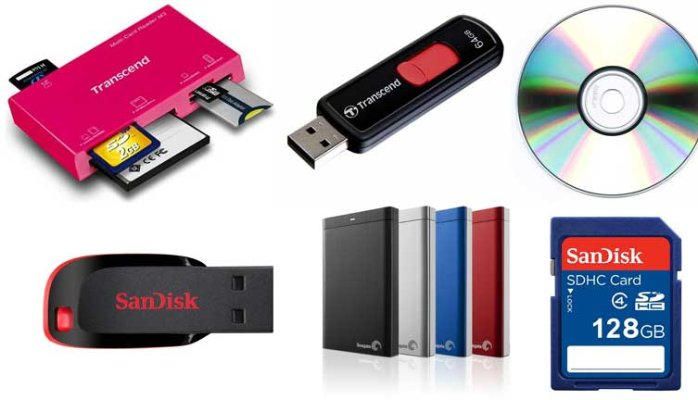
\includegraphics[width=1\texwidht]{figures/storage.jpg}}
\caption{contoh storage}
\label{storage}
\end{figure}





\section{Pengertian Storage}

Storage merupakan salah satu perangkat yang digunakan untuk menyimpan hasil dari pemprosesan data dan sistem operasi. Storage biasanya terdapat didalam komputer,storage ini bisa disebut juga dengan secondary storage.
Storage device dibagi menjadi dua bagian yaitu internal dan eksternal. internal storage device contohnya seperti Hard Disk. Internal Storage ini terdapat dalam komputer. sedangkan Eksternal Storage Device adalah suatu penyimpanan data tambahan pada komputer yang terletak diluar komputer,contohnya Hard Disk Eksternal,Flash Disk,Floppy Disk atau biasa kita sebut disket.
dalam suatu artikel menyebutkan bahwa storage merupakan penyimpanan \cite{weiser1999personal}

\section{Sejarah Storage}
Pada tahun 1725 ada seorang tokoh bernama basile bounchon yang merancang sebuah media untuk menyimpan data.Bouchon menggunakan kertas berforasi untuk menyimpan pola yang digunakan pada kain.Namun penemuannya itu baru dipatenkan pada tahun 1884 oleh Herman Hollerith.Penemuan Bouchon ternyata sangat berguna,terbukti,penemuannya digunakan selama lebih dari 100 tahun hingga pertengahan 1970.Penemuannya ini diberi nama punch card,sebuah media penyimpanan yang memiliki 90 kolom.Namun,jumlah data yang tersimpan dalam media tersebut sangatlah kecil dan fungsi utamanya bukan untuk menyimpan data melainkan untuk menyimpan pengaturan atau setting untuk mesin yang berbeda.Pada tahun 1864 Alexander Bain menemukan penemuan baru,paper tape yang biasanya digunakan untuk mesin faksimil atau telegram,dia modifikasi sehingga dapat menyimpan data.Penemuannya ini dinamakan punch tape,ada beberapa keunggulan yang didapat dari punch tape ini.Punch tape dapat menyimpan data lebih signifikan dibandingkan punch card.Barulah pada tahun 1946 ada sebuah perangkat penyimpanan yang dapat menyimpan data dengan mencantumkan ukuran tertentu,yaitu selectron Tube.Selectron Tube merupakan awal format memori komputer selectron.Dulunya harga selectron tube ini sangat mahal dan langja di pasaran.Kemudian pada tahun 1970 banyak orang yang sudah mengenal kaset dan menggunakannya untuk menyimpan data.Kaset ini merupakan terobosan yang sangat bagus karena lebih memudahkan pengguna untuk menyimpan data.Kaset ini bisa menyimpan data mulai dari 700kb sampai 1mb.
Seiring berkembangnya zaman dan ilmu pengetahuan,maka storage device ini terus berkembang dan semakin banyak pula ruang yang disediakan untuk menyimpan  data.Untuk pertama kalinya ada hard drive yang dapat menyimpan data sampai 500GB.Tiap tahunnya selalu saja ada kemajuan dan semakin bertambah besar ruangan yang disediakan untuk menyimpan data ini.Sampai saat ini tentu semakin banyak jenis-jenis storage device dan semakin mudah juga para pengguna menggunakannya,bahkan ukurannya juga ada yang kecil sehingga mudah untuk dibawa kemana-mana.

\section{Macam-macam storage Device}

1.Hard Disk Drive

Hard disk merupakan salah satu media penyimpanan data pad komputer yang terdiri dari kumpulan piringan magnetis keras dan berputar,serta komponen elektronik lainnya.Hard disk menggunakan piringan datar yang disebut dengan platter yang pada kedua sisinya dilapisi dengan suatu material yang dirancang agar bisa menyimpan informasi secara magnetis.Platter ini berputar dengan kecepatan tinggi.Setiap permukaan pada platter menampung sati milyar bit data,setiap platter menyimpan informasi dalam lingkaran-lingkaran yang disebut dengan track.Tiap track dipotong-potong lagi menjadi beberapa bagian yang disebut dengan sector.Seperti yang disebutkan di \cite{wahyudi2005mengenal}

2.Floppy Disk

Floppy disk drive adalah suatu perangkat penyimpanan yang ada didalam komputer yang dapat menyimpan data dalam kapasitas rendah.Dalam satu komputer bisa terdapat dua floppy sekaligus,tapi biasanya hanya terdapat satu floppy saja yaitu floppy A. Semua jenis floppy dilengkapi dengan unit mekanis seperti driver disk dan head positioner,Drive disk inilah yang membuat disk berputar.selain dapat menyimpan data didalam disket,floppy disk juga dapat untuk boating komputer.Seperti yang disebutkan di \cite{horie1987floppy}
3.Compact Disk

Compact disk ini biasa kita singkat CD adalah sebuah piringan kompak dari jenis piringan optik yang dapat menyimpan data.Compact Disk ini dapat menyimpan data sebesar 700 MB.Untuk membaca CD ini, alat yang diperlukan adalah CD DRIVE.CD ini bersifat hanya dapat dibaca tetapi tidak dapat ditulis,tetapi pada perkembangan terkini CD ini dapat ditulis.Seperi yang disebutkan di \cite{ernst1998turtles}

4.Flashdisk

Flashdisk adalah suatu perangkat penyimpanan yang dibuat perangkat dengan minimalis dengan ukuran kecil dengan kapasitas tertentu. Flashdisk ini dibuat dengan
mudah dan simpel karena perangkat ini sangat mudah sekali dipakai dan dibawa kemana saja. Selain itu komponen flashdisk ini mendukung usb 2.0 dan usb 3.0 tergantung
versi base yang dibuat oleh perusahaan flashdisk tersebut. Flashdisk ini mempunyai kapasitas pertama kali diluncurkan dengan ukuran 1 GB dan seiring waktu berjalan
Kapasitas ini semakin diperbesar oleh penemu flashdisk ini hingga 2 tb saat ini. Kecepatan Reading Flashdisk ini berkisar antara 1Mb/s sampai dengan 12Mb/s.Seperti yang disebutkan di \cite{aini2010mengukur}

Flashdisk ini dikatakan bahwa flash yang artinya melakukan read and scan, dan disk artinya perangkat storage. Jadi Flashdisk ini bekerja secara Read and Scan untuk
menganalisa isi perangkat tersebut apabila anda menghubungkan sesuai driver usb sesuai dukungan devices. Harga Flashdisk ini dikalangan masyarakat relatif murah
kisaran antara Rp 30ribu sampai dengan Rp 100ribu.Selain memudahkan pengguna,terkadang ukuran flashdisk yang kecil membuat penggunanya lupa menyimpan,bahkan ada yang sampai tercuci di mesin cuci.

5.Memory Card

Memory Card atau kartu memory adalah sebuah alat yang digunakan untuk menyimpan data.Ukuran memory card ini bermacam-macam,mulai dari 126 MB sampai 16 GB.Kartu memori ini ukurannya kecil,tapi dapat menyimpan data dengan ukuran yang besar,terdapat beberapa jenis ukuran memori,tetapi biasanya kartu memori mempunyai ukuran standar bit digital yaitu 16MB,32MB,64MB,128MB,256MB dan seterusnya kelipatan dua.Bukan hanya data dokumen tetapi memori juga bisa menyimpan gambar,video ataupun audio.Ukuran dari memory card sangat kecil,sehingga banyak sekali orang yang kehilangan memory,untuk mengantisipasinya,sebaiknya memory card jangan terlalu sering dilepas dari perangkat anda.

6.Magnetic Tape

Magnetik Tape adalah suatu media perekam yang terdiri dari gulungan tape halus yang terbuat dari bahan magnetis,karena itulah sering disebut dengan tape magnetis,bentuknya menyerupai tape yang biasa kita pasang diradio zaman dulu.Akan tetapi fungsinya memang seperti tape musik zaman dulu karena tape magnetis ini dapat merekam suara juga.Namun kendala pada tape jenis ini adalah mudah rusak,apalagi jika gulungan magnetisnya sampai berantakan,seperti tape kaset radio.


\section{keunggulan dan kekurangan storage internal}

Storage internal mempunyai keunggulan tersendiri daripada storage eksternal,karena storage internal tersimpan didalam maka tidak mungkin bagi storage internal ini menghilang secara tidak sengaja dari perangkat anda.Dalam komputer anda biasanya terdapat ruang penyimpanan seperti data E,data C dan data D,sebenarnya itu merupakan salah satu keunggulan storage internal yang kuat untuk dipartisi hingga beberapa bagian.Jika anda memindahkan file pun akan lebih cepat menggunakan storage internal karena mempunyai kemampuan write and read yang lebih cepat.Dan yang paling penting storage internal ini mempunyai umur yang panjang atau lebih tahan lama.

\section{keunggulan dan kekurangan storage eksternal}

Storage eksternal yang mempunyai ukuran lebih kecil tentu memudahkan pemiliknya untuk membawanya kemana-mana,namun karena ukurannya kecil,storage eksternal ini sering hilang.Walaupun bentuknya kecil,storage eksternal ini mempunyai kapasitas yang tak kalah besar daripada storage internal bahkan beberapa storage eksternal bisa mempunyai kapasitas melebihi storage internal.Storage eksternal ini terletak diluar,jadi walaupun rusak,kamu dapat dengan mudah menggantinya.Walaupun begitu kemungkinan besar kehilangan atau lupa menaruh storage jenis ini sangat besar sekali dikarenakan ukurannya yang kecil.Selain itu storage eksternal ini juga cepat rusak karena banyak sekali kemungkinan yang bisa membuat storage eksternal ini rusak seperti tercuci dan berkarat.Terlalu sering digunakan juga bisa menjadi penyebab storage eksternal ini lebih cepat rusak.Karena terletak diluar,maka proses mengcopy file melalui storage eksternal ini sangat lambat,ini disebabkan kemampuan write and ride nya yang kurang cepat.Seseuai dengan harganya yang lebih murah,sudah tentu storage eksternal ini mempunyai kekurangan lebih banyak daripada storage eksternal dari segi ketahanannya dan kemampuannya,tetapi storage jenis ini juga mempunyai keunggulan yang tidak ada di storage internal.

\section{Kesimpulan}

Storage device adalah media penyimpanan data dengan berbagai jenis,bentuk dan ukuran.Jenis dari storage terbagi dua,yaitu storage device internal dan storage device eksternal,storage device internal mempunyai keunggulan yaitu tahan lama dan lebih cepat saat membaca data dan aman karena terletak didalam pc maka storage internal tidak mudah hilanag.Sedangkan storage eksternal yang terletak diluar sangat rawan terjadi kehilangan karena bentuknya yang kecil,storage eksternal juga mudah rusak karena banyak kemungkinan yang terjadi pada storage jenis ini seperti tercuci ataupun jatuh.Kekurangan yang lain dari storage ini adalah lambat pada saat proses pembacaan data oleh komputer.masing-masing storage mempunyai keunggulan tersendiri dan bentuknya pun beragam,ada yang besar dan ada juga yang sangat kecil.Untuk ruang penyimpanan itu sendiri bermacam-macam mulai dari ukuran beberapa byte sampai tera.Sampai saat ini masih dicari storage yang lebih memanjakan para penggunanya agar lebih aman,mudah dibawa,tidak mudah hilang tetapi dengan kapasitas yang besar.








%%%%%%%%%%%%%%%%%%%%%%%%%%%%%%%%%%%%%%%%%%%%%%%%%%%%%%
%% optional prologue or prologues
% \chapter{Chapter Title}
% \prologue{<text>}{<author attribution>}

%%%%%%%%%%%%%%%%%%%%%%%%%%%%%%%%%%%%%%%%%%%%%
% Edited Book: Author and Affiliation
%%%%%%%%%%%%%%%%%%%%%%%%%%%%%%%%%%%%%%%%%%%%%

% After \chapter{Chapter Title}, you can
% enter the author name and embed the affiliation with
% \chapterauthors{(author name, or names)
% \chapteraffil{(affiliation or affiliations)}
% }    

% For instance:
% \chapter{Chapter Title}
% \chapterauthors{G. Alvarez and R. K. Watts
% \chapteraffil{Carnegie Mellon University, Pittsburgh, Pennsylvania}

% For separate affiliations you can use \affilmark{(number)} after
% the name of a particular author and before the matching affiliation:

% For instance:
% \chapter{Chapter Title}
% \chapterauthors{George Smeal, Ph.D.\affilmark{1}, Sally Smith,
% M.D.\affilmark{2}, and Stanley Kubrick\affilmark{1}
% \chapteraffil{\affilmark{1}AT\&T Bell Laboratories
% Murray Hill, New Jersey\\
% \affilmark{2}Harvard Medical School,
% Boston, Massachusetts}
% }

%%%%%%%%%%%%%%%%%%%%%%%

%% short version of section head, or one without \\ supplied in sq. brackets.

% \section[Introduction and fugue]{Introduction\\ and fugue}
% \subsection[This is the subsection]{This is the\\ subsection}
% \subsubsection{This is the subsubsection}
% \paragraph{This is the paragraph}

% \begin{chapreferences}{widest label}
% \bibitem{<label>}Reference
% \end{chapreferences}

% optional chapter bibliography using BibTeX,
% must also have \usepackage{chapterbib} before \begin{document}
% Must use root file with \include{chap1}, \include{chap2} form.
%\bibliographystyle{plain}
%\bibliography{<your .bib file name>}

% optional appendix at the end of a chapter:
% \chapappendix{<chap appendix title>}
% \chapappendix{} % no title

%%%%%%%%%%%%%%%%%%%%%%%%%%%%%%%%%%%%%%%%%%%%%%%%%%%%%%%%%%%%%%%%
%% End Matter >>>>>>>>>>>>>>>>>>

% \appendix{<optional title for appendix at end of book>}
% \appendix{} % appendix without title

% \begin{references}{<widest label>}
% \bibitem{sampref}Here is reference.
% \end{references}

%%%%%%%%%%%%%%%%%%%%%%%%%%%%%%%%%%%%%%%%%%%%%%%%%%%%%%%%%%%%%%%%
%% Optional Problem Sets: Can use this at the end of each chapter or at end
%% of book

% \begin{problems}
% \prob
% text

% \prob
% text

% \subprob
% text

% \subprob
% text

% \prob
% text
% \end{problems}

%%%%%%%%%%%%%%%%%%%%%%%%%%%%%%%%%%%%%%%%%%%%%%%%%%%%%%%%%%%%%%%%
%% Optional Exercises: Can use this at the end of each chapter or at end
%% of book

% \begin{exercises}
% \exer
% text

% \exer
% text

% \subexer
% text

% \subexer
% text

% \exer
% text
% \end{exercises}


\bibliographystyle{IEEEtran}
\bibliography{IEEEabrv,windows,linux,mac,bsd,android,dosunix,software,definisi,kernel,hardware}

%%%%%%%%%%%%%%%%%%%%%%%%%%%%%%%%%%%%%%%%%%%%%%%%%%%%%%%%%%%%%%%%
%% INDEX: Use only one index command set:

%% 1) The default LaTeX Index
\printindex

%% 2) For Topic index and Author index:

% \usepackage{multind}
% \makeindex{topic}
% \makeindex{authors}
% \begin{document}
% ...
% add index terms to your book, ie,
% \index{topic}{A term to go to the topic index}
% \index{authors}{Put this author in the author index}

%% (these are Wiley commands)
%\multiprintindex{topic}{Topic index}
%\multiprintindex{authors}{Author index}

\end{document}
